\documentclass[review]{elsarticle}

\usepackage{lineno,hyperref}
\usepackage{amsmath}
\usepackage{booktabs}
\usepackage{color}
\usepackage[usenames,dvipsnames]{xcolor}

\modulolinenumbers[1]

\journal{Journal of \LaTeX\ Templates}

%%%%%%%%%%%%%%%%%%%%%%%
%% Elsevier bibliography styles
%%%%%%%%%%%%%%%%%%%%%%%
%% To change the style, put a % in front of the second line of the current style and
%% remove the % from the second line of the style you would like to use.
%%%%%%%%%%%%%%%%%%%%%%%

%% Numbered
%\bibliographystyle{model1-num-names}

%% Numbered without titles
%\bibliographystyle{model1a-num-names}

%% Harvard
%\bibliographystyle{model2-names.bst}\biboptions{authoryear}

%% Vancouver numbered
%\usepackage{numcompress}\bibliographystyle{model3-num-names}

%% Vancouver name/year
\usepackage{numcompress}\bibliographystyle{model4-names}\biboptions{authoryear}

%% APA style
%\bibliographystyle{model5-names}\biboptions{authoryear}

%% AMA style
%\usepackage{numcompress}\bibliographystyle{model6-num-names}

%% `Elsevier LaTeX' style
\bibliographystyle{elsarticle-num}
%%%%%%%%%%%%%%%%%%%%%%%
\usepackage{setspace}
\doublespacing
\begin{document}

\newcommand{\edit}[1]{\textcolor{blue}{#1}}

\begin{frontmatter}

\title{Forecasting vegetation condition for drought early warning systems in pastoral communities in Kenya}


%% Group authors per affiliation:
%\author{Elsevier\fnref{myfootnote}}
\author{Adam B. Barrett$^{a,b}$, Steven Duivenvoorden$^{a,c}$, Edward Salakpi$^a$, James M. Muthoka$^{d}$, Seb Oliver$^{c,a}$ and Pedram Rowhani$^{d}$*}
\address{
	$^{a}$ \quad The Data Intensive Science Centre, Department of Physics and Astronomy, University of Sussex, Brighton BN1 9QH, UK\\
	$^{b}$ \quad Sackler Centre for Consciousness Science, Department of Informatics, University of Sussex, Brighton BN1 9QJ, UK \\
	$^{c}$ \quad Astronomy Centre, Department of Physics and Astronomy, University of Sussex, Brighton BN1 9QH, UK\\
	$^{d}$ \quad School of Global Studies, Department of Geography, University of Sussex, Brighton, BN1 9QJ, UK \\
	Corresponding author: P.Rowhani@sussex.ac.uk
	}




%% or include affiliations in footnotes:
%\author[mymainaddress,mysecondaryaddress]{Elsevier Inc}
%\ead[url]{www.elsevier.com}

%\author[mysecondaryaddress]{Global Customer Service\corref{mycorrespondingauthor}}
%\cortext[mycorrespondingauthor]{Corresponding author}
%\ead{support@elsevier.com}

%\address[mymainaddress]{1600 John F Kennedy Boulevard, Philadelphia}
%\address[mysecondaryaddress]{360 Park Avenue South, New York}


\begin{abstract}
{\color{red} Live version, post 1st review, pre resubmission}

Droughts are a recurring hazard in sub-Saharan Africa, that can wreak huge socioeconomic costs. Acting early based on alerts provided by early warning systems (EWS) can potentially provide substantial mitigation in terms of money and lives lost. However existing EWS tend only to monitor, rather than forecast, the environmental and socioeconomic indicators of drought, and hence are not always sufficiently timely to be effective in practice. Here we make {\color{red} a first attempt [is it really first?, Seb]} at forecasting satellite-based indicators of vegetation condition that are commonly monitored. Specifically, we forecast the Normalized Difference Vegetation Index (NDVI) and the Vegetation Condition Index (VCI) over pastoral livelihood zones in Kenya as these are the common indicators used by the National Drought Management Authority (NDMA). Using data from MODIS and Landsat, we apply linear autoregression and Gaussian processes modeling methods and demonstrate accurate forecasting several weeks ahead. We explored predicting the drought alert marker used by NDMA (3 month VCI$<35$). Both of our models were able to predict this alert marker four weeks ahead with a hit rate of around 89\% and a false alarm rate of around 4\%, or 81\% and 6\% respectively six weeks ahead. The methods developed here can identify a deteriorating vegetation condition well in advance and thus help disaster risk managers act early to support vulnerable communities and limit the impact of a drought hazard.
\end{abstract}

\begin{keyword}
Landsat; MODIS; Gaussian Processes; Drought; NDVI; VCI
\end{keyword}

\end{frontmatter}

\linenumbers

\section{Introduction}

Droughts are a major threat globally as they can cause substantial damage to society, especially in regions that depend on rain-fed agriculture. They particularly impact food security by significantly reducing agricultural production \citep{Lesk} and raising food prices \citep{Nelson3274,BROWN201531}, which often leads to increased levels of malnutrition, migration, disease, and other health concerns \citep{10.1093/rsq/hdr006,Stanke}. Since 2000, there have been 319 drought events reported (EMDAT 2019), which together have killed over 21,000 people and affected almost 1.4 billion others. The majority of these events took place in sub-Saharan Africa where many communities rely on predictable rainfall patterns for their livelihood. 


In East Africa, the main economic activity in the arid and semi-arid lands (ASAL) is subsistence rain-fed agriculture, as well as livestock farming using pastures and grasslands as the main source of fodder. The pastoral and agro-pastoral communities who live in these drylands have dealt with rainfall variability and drought over centuries by developing extensive adaptation and mitigation strategies to reduce their vulnerability to these shocks \citep{Nyong2007,orindi2007pastoral}. However, in recent years these communities have seen their coping strategies compromised by population growth and land use change \citep{Galvin2001ImpactsOC}. Additionally, while there is some uncertainty in the climate models \citep[IPCC,][]{stocker2013climate}, rainfall variability is expected to increase in the region \citep{Tierneye1500682,yang2018brief}. These factors in combination will make it harder for indigenous knowledge systems to deal with droughts, and exacerbate the problems created by droughts.  Governments and donor agencies in the region have thus developed several tools and early warning systems (EWS) to mitigate the impact of droughts on pastoralists.


Most EWS tend to monitor current key biophysical and socio-economic factors to assess the possible exposure of vulnerable people to specific hazards. However, once the impacts are visible, it will be too late to mitigate the consequences \citep{kogan}. \edit{As a consequence,} being better prepared before a drought hits significantly reduces the costs and losses from these disasters \citep{venton2012economics}. Hence, EWS now increasingly include expert knowledge and qualitative assessments of seasonal climate forecasts to assess the future development of food security, and define actions to mitigate possible losses \citep{nhess-15-895-2015,TozierdelaPoterie2015}. 

Within East Africa, the Famine Early Warning Systems Network (FEWS NET) monitors food security through data collection and a deep understanding of the livelihood patterns in the region. A team of experts and analysts will also look at seasonal climate forecast to estimate future food security outcomes using scenario development \citep{FEWS}. In Kenya, the drought EWS operated by the National Drought Management Authority (NDMA) provides monthly bulletins assessing food security in the 23 ASAL regions \edit{using current}  environmental (rainfall, vegetation condition) and socio-economic (production, access, and utilisation) factors. Based on these factors, the bulletins include a qualitative evaluation of food security outcomes in the months ahead. {\color{red} Shouldn't the next sentence be in the discussion, not here, because we are not addressing consequences in this paper and also our premise is that the current EWS do not forecast at all [Seb]}. However, EWS should move from forecasting hydro-meteorological events toward estimating the expected consequences of hazards, i.e. impact-based forecasting, to identify more effective early action protocols \citep{wmo2015wmo,nhess-2018-26}.

Pastoralists strongly rely on forage availability to keep their livestock. \edit{Existing EWS provide information on pasture condition through the use of satellite-based Earth observation derived vegetation indices,} such as the Normalized Difference Vegetation Index (NDVI) and the Vegetation Condition Index  \citep[VCI,][]{KOGAN199591,rs8040267,RULINDA201132,ROJAS2011343}. These products are commonly used as drought indicators as they provide timely and regular assessment of vegetation health over large spatial areas. EWS should include a forecast of these indicators as it would allow local and national stakeholders to act early and support the pastoralists in times of drought. Recent studies have highlighted the potential of satellite-based earth observation data to forecast agricultural productivity \citep{ZAMBRANO201815} and seasonal forage availability \citep{VRIELING201644}.

The main goal of this paper is to explore methods to forecast (\edit{up to six weeks ahead}) the vegetation indices that are commonly used in the pastoral areas of Kenya to monitor droughts. We specifically aim to estimate the potential to forecast NDVI and the 3-month VCI (VCI3M), as used by the NDMA in their monthly bulletins. \edit{The indices are extracted from data derived from the Landsat mission (every 16 days at 30\,m resolution and the MODerate resolution imaging Spectroradiometer (MODIS - daily data at 500\,m resolution).}

\edit{Machine-learning techniques offer a data-driven, empirical route to these forecasts. Many different data inputs could be used to forecast these vegetation indices (e.g. precipitation and precipitation forecasts. However, perhaps the most simple is to use the past history of the indices themselves. This has the practical benefits of readily available data over large areas. It is also likely to work as these indices are subject to plant growth and climate cycles giving periodic behaviour on large temporal scales that can be empirically modelled while external perturbations, such as water availability, have persistent impact providing correlations on short temporal scales. The existing EWS itself implies that the indices have forecasting power as moderately low indexes are labelled ``alert" implying they might precede lower ``alarm" levels. }
{\color{red} something about the Boku paper here}}

\edit{The machine-learning techniques we attempt are Gaussian Process regression \cite[GP,][]{gpm} w), and linear autoregressive (AR) modelling \citep[e.g.][]{Hamilton94}.} GP regression uses kernel-based non-parametric Bayesian inference on the structure of correlations between observations, and is widely applied to classification, interpolation, change detection and forecasting problems \citep{955315,Chandola2010SCALABLETS,7487896,rs11050481}. For an overview on the principles of GPs, and how they have previously been applied throughout remote sensing, see \cite{7487896}. Linear AR is the regression of future observations on past observations, assuming a linear dependence. This has previously been performed on monthly (i.e.~temporally more sparse) NDVI data, see for example \cite{Asoka:2015} and \cite{Papagiannopoulou}, with mixed results in terms of forecasting potential ($R^2$-scores between 0 and 0.4 at a lead time of one month).  

{\color{red} I think this introduction needs something to end on that leads into the paper better}

\section{Study area}
About 80\% of Kenya lies within the ASALs, and the main economic activity in these regions is livestock farming \citep{UNDP2013,FAO2014}. The livestock sector accounts for 13\% of the national GDP and 43\% of its agricultural GDP. Pastures and grasslands in the ASAL serve as the main source of fodder for the pastoral communities in Kenya \citep{Behnke2011}. Following several periods of intense drought, the government in Kenya established the NDMA in 2016, to set up and operate a drought early warning system (DEWS), as well as to establish drought preparedness strategies and contingency plans (GoK). One key biophysical indicator used by the NDMA drought phase classification is the VCI \citep{rs8040267}, which is measured at county level as well as over the different livelihood zones within the county (FEWS NET 2011). This study focused on the 10 (agro)-pastoral livelihood zones (see Fig \ref{fig:l_zone}), which cross 15 counties. The names of the 29 livelihood zone county intersections can be found in Appendix \ref{app}. FEWS NET shape files were used to define these regions, and to demarcate the Landsat and MODIS pixels from which to sample data.




\begin{figure}
	\centering
	\includegraphics[trim = 45mm 0mm 0mm 0mm,width=14.0 cm]{figures/livelihood_zones13.pdf} 
	\caption{Maps of Kenya showing (A) the livelihood zones from which pixels were sampled for analysis, and (B) land cover classification (according to the MODIS MCD12Q1 map). Analyses were performed for 29 regions, defined by pastoral livelihood zone and county intersections. For the MODIS data only those pixels identified as being from grassland are used.} \label{fig:l_zone}
\end{figure}





\section{Data} \label{sec:data}

\abb{This section describes the two datasets. A comparison between them, and justification of data selection can be found in Section XXX in the Supplementary Material.}

\subsection{Landsat}
Landsat-5, 7 and 8 \citep{royetal} red and near infrared (NIR) surface reflectances and quality assessment (QA) data over the 10 pastoral livelihood zones of Kenya, from 1/1/2000 to 1/2/2019, were obtained using the United States Geological Survey (USGS) EarthExplorer. Specifically, data were drawn from the Level-1 Precision Terrain (L1TP) processed dataset, which has well-characterized radiometry and is inter-calibrated across the different Landsat sensors. The QA data indicate whether or not each observation is affected by cloud; only observations classified as clear were kept. The spatial resolution of these data is 30m and the repeat interval is 16 days. Landsat-5 data were available up until November 2011 (albeit with several large gaps), Landsat-7 data were available for the whole time-period, and Landsat-8 data were available from March 2013. 
\edit{The surface reflectances} were combined to obtain NDVI \edit{according to the usual formula.} From each of the 29 pastoral livelihood zone and county intersections (see Fig. \ref{fig:l_zone}), 1\,000 random pixels were selected for analysis, \edit{out of those for which at least half of the observations were present and labelled good quality.}\footnote{\edit{Except for a few regions, for which this threshold had to be dropped in order to be able to obtain 1\,000 pixels, see Table \ref{tab:NDVI_LS} in the Appendix.}} 

% We note that the red and NIR bands are defined by slightly different spectral ranges for the different Landsat missions, and that this can lead to slightly different NDVI values for the same vegetation. More specifically, Landsat-8 measures slightly higher values for the NDVI of dry shrub-lands than Landsat-7, while at higher values of NDVI there is more convergence \citep{LS}. The data from all three Landsat missions where used to train the GP's (see Section \ref{sec:Method}).

\subsection{MODIS}
\edit{NDVI data were also} obtained from the MODIS Terra/Aqua Nadir BRDF-Adjusted Reflectance (NBAR) product \citep[MCD43A4,v006;][]{Schaaf2015} via the NASA Land Processes Distributed Active Archive Center (LP DAAC) using Application for Extracting and Exploring Analysis Ready Samples (AppEEARS), from \edit{the start date, 22/2/2000, up to 1/2/2019.} The spatial resolution of \edit{this product} is 500m and the repeat interval is 1 day, \edit{with the daily data being 16 day composites of raw observations at 1 to 2 day intervals}. From each of the 29 pastoral livelihood zone and county intersections, 100 random pixels were selected for analysis, out of those pixels identified as being from grassland according to the MODIS land cover classification maps (MCD12Q1,v006).

\section{\edit{Pre-processing}}

\subsection{Temporal gridding and gap-filling} \label{gap}
To prepare the datasets for the testing of forecasting, each NDVI time series was processed into a form containing, wherever possible, precisely one observation every 7 days. For the MODIS data, the mean of all reliable \edit{data} was taken for each week. For the Landsat data, this required compilation and interpolation of data sampled every 16 days from up to 3 different Landsat missions. Further, gap-filling had to be carried out on both datasets whenever there was a lack of reliable observations due to cloud cover and/or instrumental malfunction. The following subsections describe briefly the gridding and gap-filling methods employed on the Landsat and MODIS data, respectively. \edit{Further details and justification of these methods can be found in the Supplementary Material, Section XXX.}

\subsubsection{Gridding and gap-filling on Landsat data using Gaussian Processes}

Gridding and gap-filling on the Landsat data was done using Gaussian Process (GP) modelling; \edit{for details see Section XXX in the Supplementary Material. For a given pixel, the GP modelling took raw data as input, fit a temporal correlation structure to the data, and used this to output a time series of expected NDVI values, with observations on every Saturday from 1/1/2000 to 2/2/2019.} Two versions of GP gap-filling were carried out, which we refer to as forecast mode and non-forecast mode. For the non-forecast mode all of the data (1/1/2000 to 1/2/2019) from the given pixel were used to train the GP. The non-forecasting mode was used as the ``ground truth'' to test forecasts against. The forecast mode, by contrast, only used data up to a certain date, whichever date a forecast was being attempted from - since when doing forecasting with a near real-time data stream, one does not have access to future data. 

\subsubsection{Gridding and gap-filling on MODIS data} \label{sec:gapMODIS}


As mentioned above, gridding of the MODIS data was done by taking the mean of all reliable \edit{data} from each week. Gaps were then filled using temporal quadratic interpolation. Quadratic interpolation fills each gap using the best fit quadratic function to the two observations before the gap and the two observations after the gap (via least squares). The Savitzky-Golay \citep[SG,][]{Savitzky1964} smoothing method was then used to filter high-frequency measurement noise. SG smoothing involved, for each observation, fitting a polynomial to a window centred on the observation, and then replacing that observation with the corresponding observation on the polynomial fit. \edit{To determine the optimal window length, the polynomial order was set 2 and different windows lengths were tested as done by \cite{Chen2004, bg-10-4055-2013} }. The polynomials were fit, for each \edit{each} window \edit{length}, to the original data. {\color{red} Based on previous applications of this method to filter MODIS data \citep{bg-10-4055-2013,Chen2004}}. A sliding windows of length 7 time-steps (weeks) and a polynomial of order 2 (i.e.~quadratic function) were chosen and fitting done using least squares.

\edit{ A sliding windows of length 7 time-steps (weeks) and a polynomial of order 2 (i.e.~quadratic function) were chosen because,  a good amount of the noise was filtered out and resulting smooth NDVI time were far off the original data.}.

 A summary of the entire work from data preparation to forecasting drought can be seen in figure(\ref{fig:flowchart})
 

Since there were occasional long segments of interpolated data, where large gaps had been filled, and NDVI values sometime took unrealistic values (greater than 1 or less than 0), it was decided to remove all interpolations longer than 6 weeks, see Section \ref{sec:Lmax} in the Supplementary Material for details. 

\newpage

\begin{figure} 
	\centering
	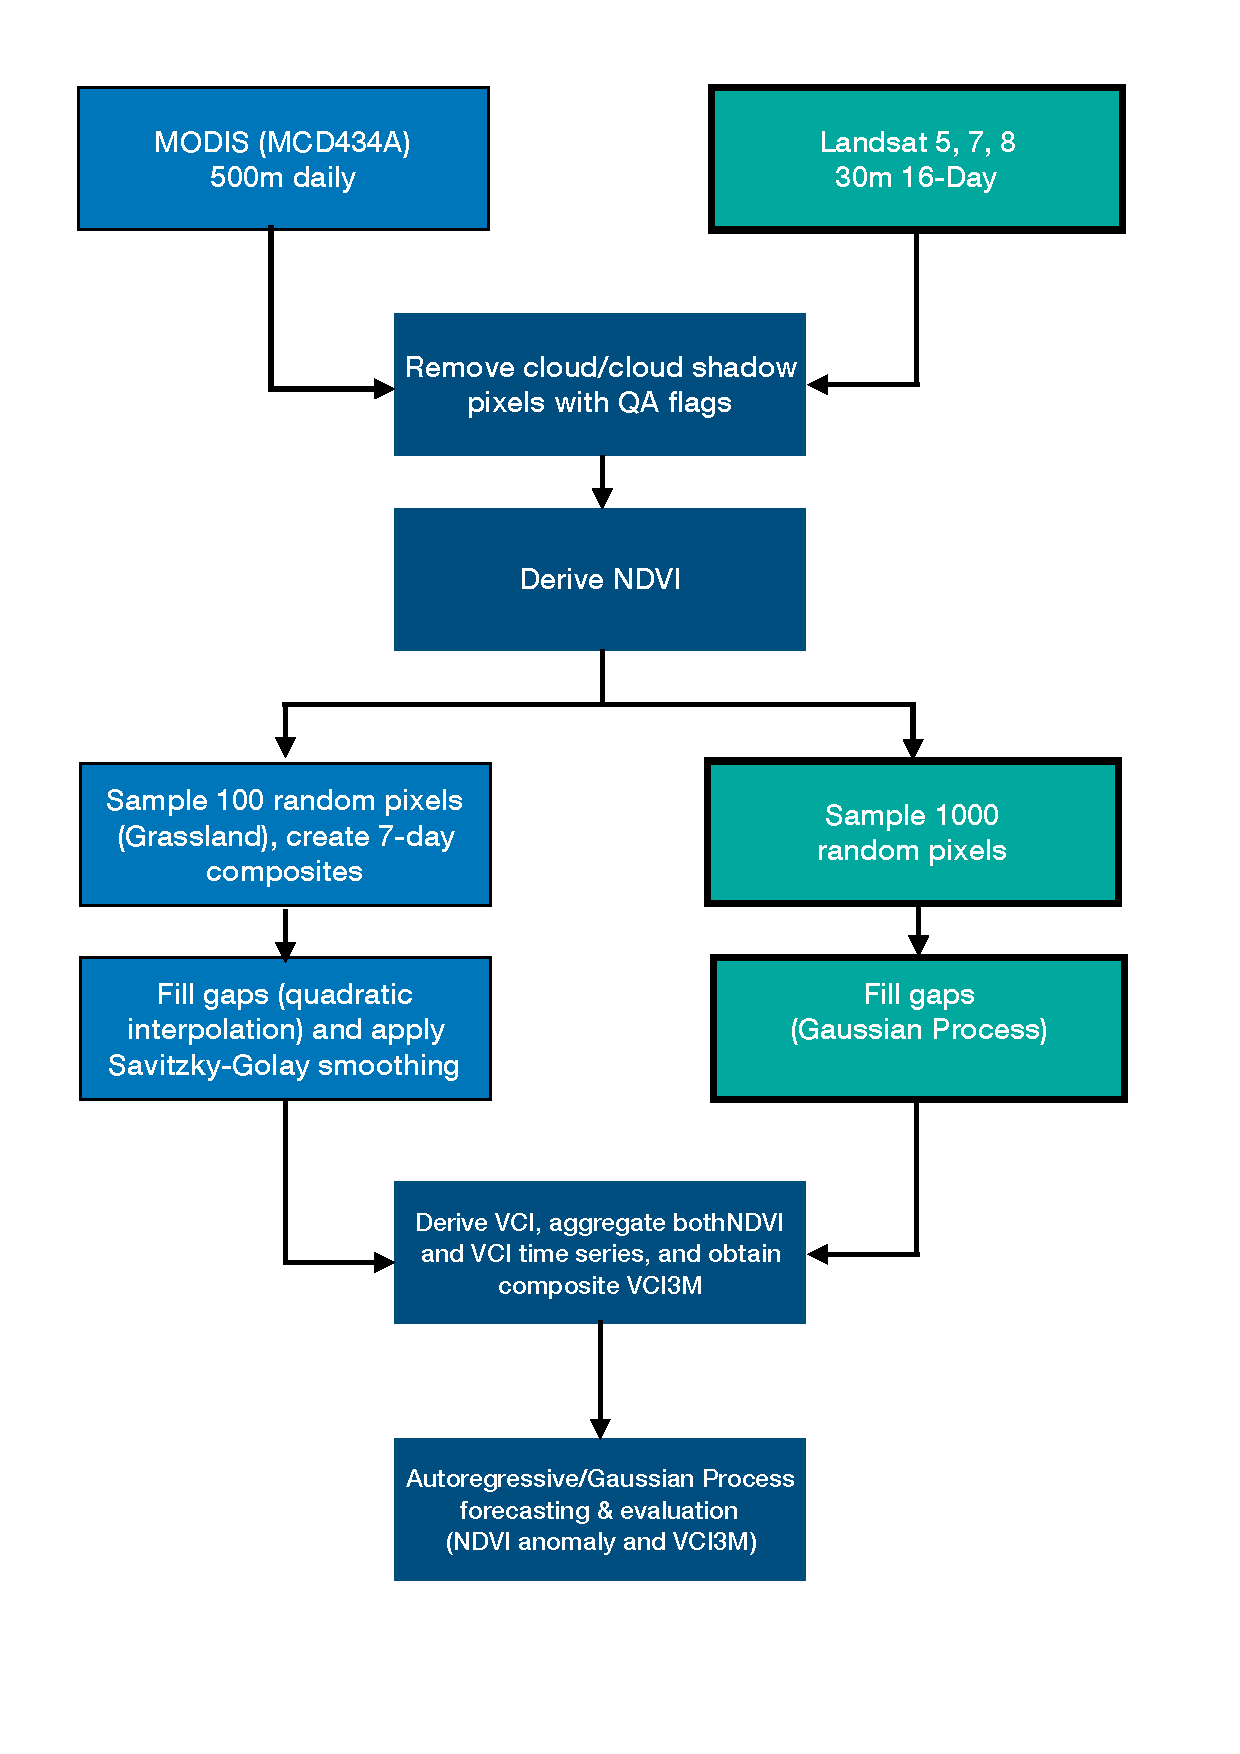
\includegraphics[trim = 10mm 0mm 0mm 0mm,width=13 cm]{figures/Flowchart.pdf}
	\caption{A Flow chart of the data processing and analysis } \label{fig:flowchart}
\end{figure}

\section{Methods}

\subsection{Forecast indices and aggregation} \label{sec:vci}
The forecast indices were \edit{(absolute)} NDVI anomaly and VCI3M. NDVI anomaly is the mean-subtracted NDVI, where the mean is the average NDVI for the given week of the year over all years covered by the data. VCI3M is the mean VCI across the 3 months leading up to the given observation time point, with VCI at time point $i$ being defined as
\begin{equation}
\rm{VCI}_i = 100 \times \frac{\rm{NDVI}_i - \rm{NDVI}_{min,i}}{ \rm{NDVI}_{max,i} - \rm{NDVI}_{min,i}},
\end{equation}
where $\rm{NDVI}_{min,i}$ and $\rm{NDVI}_{max,i}$ are the minimum and maximum values for the NDVI of the pixel in the given week over all years covered by the data. On Landsat pixels, the mean, maximum and minimum value for the NDVI for each week of the year
was computed using the non-forecast mode GP interpolated time series. Then forecast mode and non-forecast mode versions of each index were created. 

With both the Landsat and MODIS datasets, individual pixel time series for each index were aggregated, by taking the mean, within each livelihood zone and county intersection. Thus forecasting was carried out on a single time series for each region (see Fig. \ref{fig:ndvi_lk} for an example time series). With the MODIS data, since not all gaps were interpolated, whenever there were fewer than 25 individual pixel observations from a particular region at a given time point, it was decided that there should be no datum in the aggregate time series, i.e.~there should be a gap.\footnote{VCI3M is the mean of the most recent 12 weeks of VCI observations; if some of these were missing, the mean was taken over just the ones that were present. If the current observation was not present, a gap was placed in the VCI3M time series.} 



\begin{figure}
	\centering
	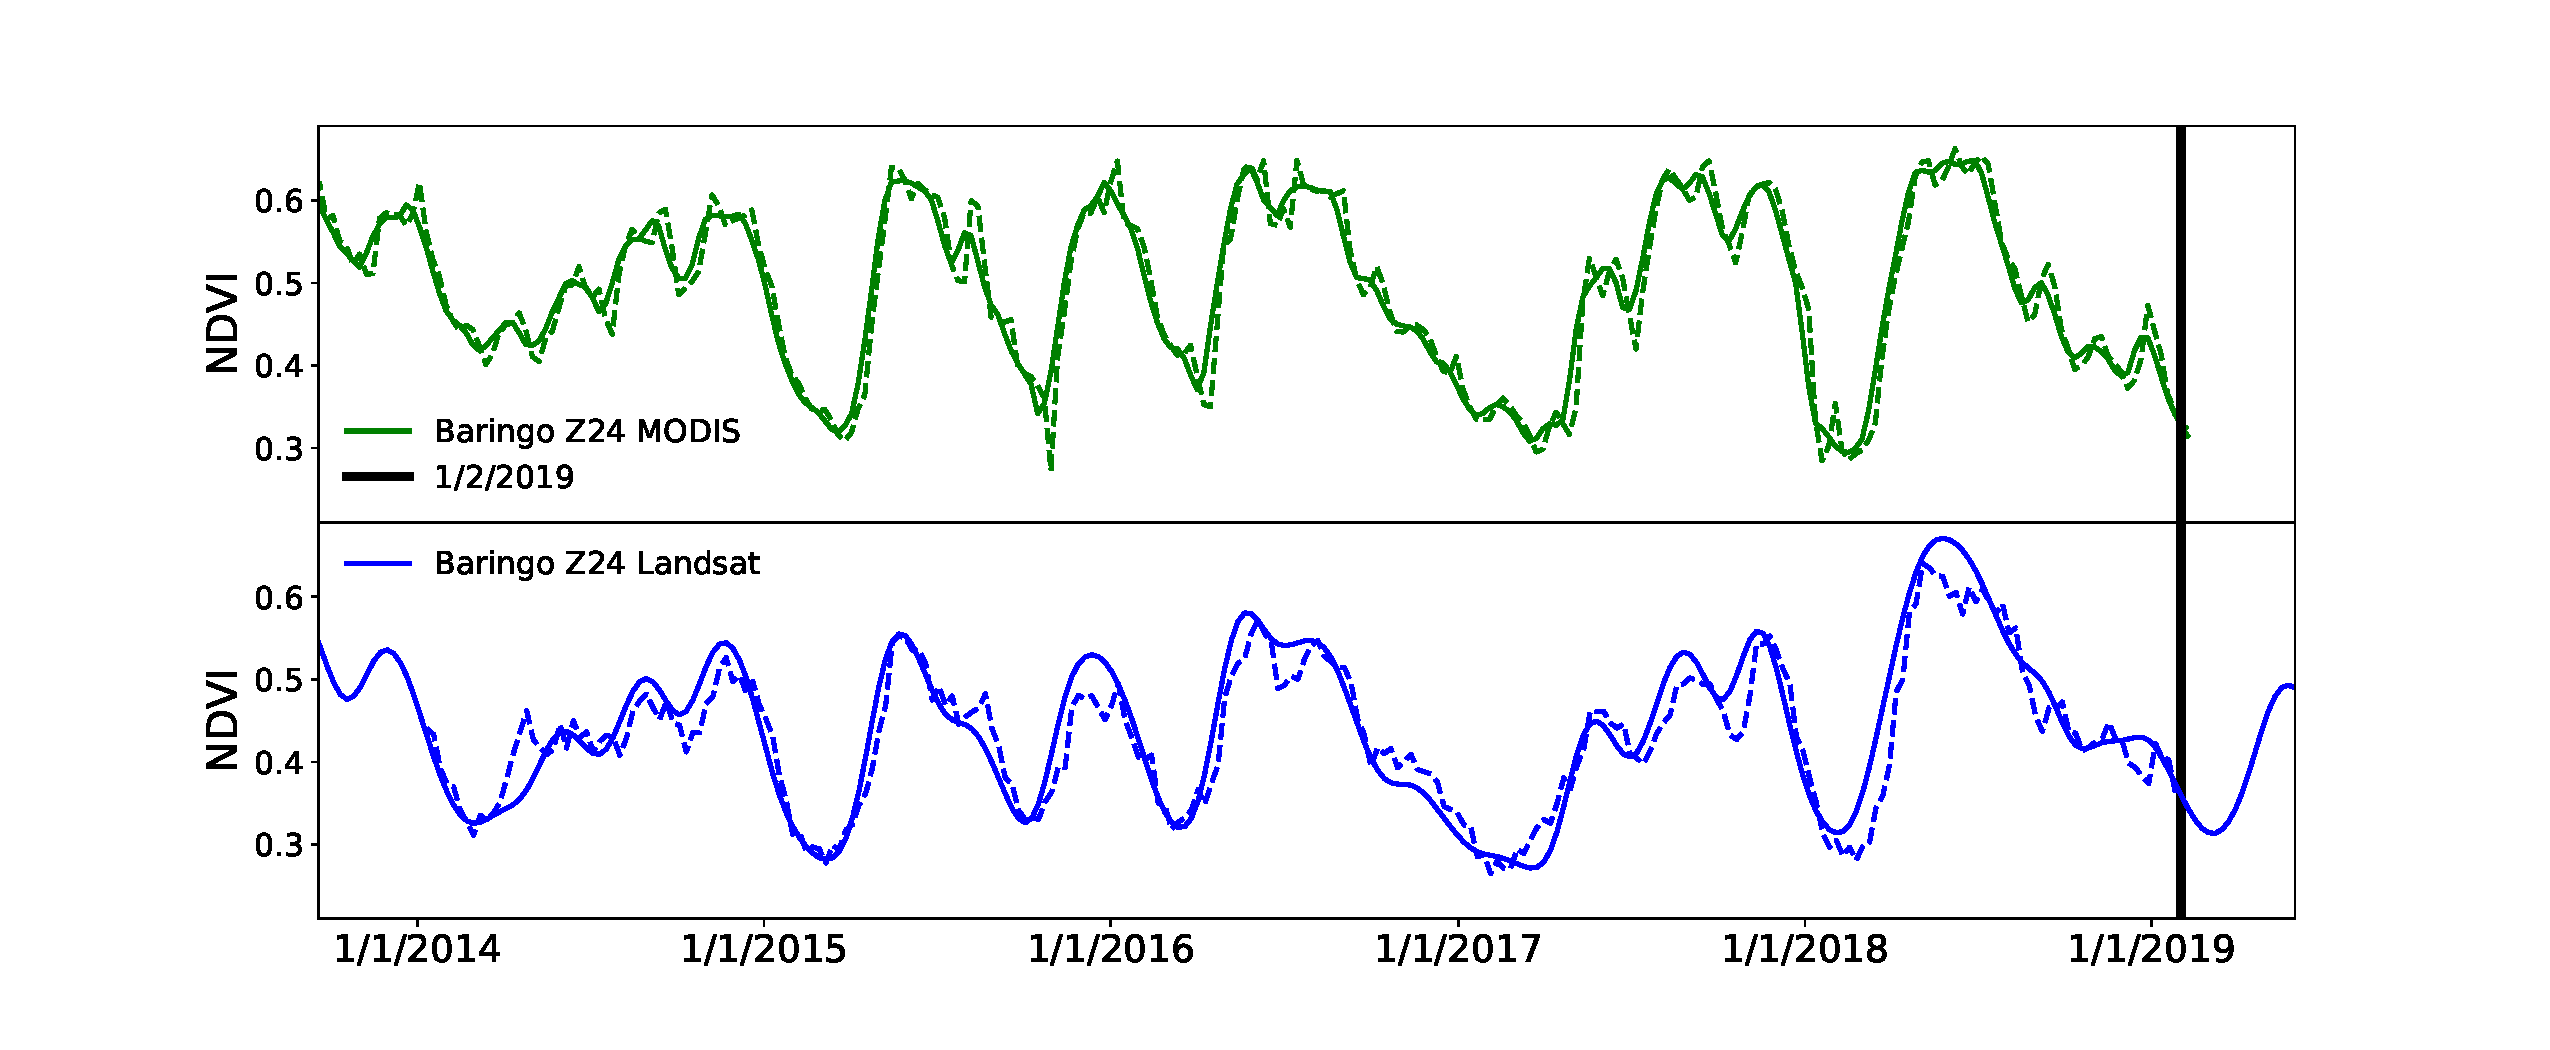
\includegraphics[trim = 50mm 0mm 0mm 0mm,width=14.5 cm]{figures/NDVI2.pdf} 
	\caption{Aggregated NDVI time series from the intersection of Baringo county and livelihood zone 24. The top panel shows MODIS data, and the bottom panel shows Landsat data (solid lines), processed using the methods described in the text. The dotted lines in each panel show forecasting at a lead time of 2 weeks, using the AR method on the MODIS data, and the GP method on the Landsat data.} \label{fig:ndvi_lk}
\end{figure}

\subsection{Forecasting}
\edit{GP forecasting was performed by GP modelling and extrapolation, see Section \ref{sec:GPM} in the Supplementary Material for details. AR forecasting was performed with the following model-fitting and extrapolation method.} For forecasting $n$ weeks ahead, the following model was fit:
\begin{equation}
X_{t+n}=\sum_{i=0}^{p-1}a_iX_{t-i}+\epsilon_t\,, \label{eq:AR1}
\end{equation}
where $X$ is NDVI anomaly (or VCI3M with mean removed), subscripts denote the observation (week), $a_i$ are model parameters, $\epsilon_t$ are the residuals (i.e.~the errors), and $p$ is the model order. Fitting the model to a segment of data involved finding the model parameters that gave the minimum sum-square error, i.e.~led to residuals with the minimum variance. To make a forecast, the model was fit using the most recent $T$ consecutive observations, and then used to predict the observation $n$ weeks after the most recent observation. This forecasting method was carried out along the entire available time series, fitting a distinct model to each segment of length $T$. A search for optimal model orders and training segment lengths found that forecast quality, as measured by root mean square error (RMSE), plateaued at $T=200$ and $p=3$.\footnote{High values of $p$ up to 20 were also explored with LASSO regression (a regularisation procedure), but this led to inferior forecasting.}



% To check that results were not strongly dependent on the choice of maximum allowed interpolation length $L_{\mathrm{max}}$ in the gap filling (see Secion \ref{sec:gapMODIS}) the method was applied to the MODIS data processed with $L_{\mathrm{max}}=4$ and 8, in addition to $L_{\mathrm{max}}=6$. As can be seen in Table \ref{tab:IL choices}, results did not substantially depend on the choice of this parameter. 

% For comparison, this method was also applied to the Landsat data. AR models were fit to the forecast mode time series, and predictions from the model were then compared to corresponding data on the non-forecast mode time series. 

\subsection{Metrics for assessing forecasts}
Several metrics were used to assess the performance of the forecast methods tested on the data. In addition to RMSE, the $R^2$-score and the percentage of standard deviation remaining, $S$, were used. These are given by:
\begin{align}
	R^2{\text -}{\rm score} &= 1 - \frac{\sum_i (y_i - f_i)^2 }{\sum_i (y_i - \bar{y})^2}, \label{eq:r2} \\
	S &= 100 \times \frac{\sqrt{ \sum_i (y_i-f_i)^2 }}{\sqrt{  \sum_i (y_i-\bar{y})^2 }} \label{eq:S}\,,
\end{align}
where the $y_i$ are the true data, and the $f_i$ are the forecasts. Note that $S\equiv 100\times\sqrt{1-R^2{\text -}\rm{score}}$. \edit{To test for bias, linear regression of actual index on forecast index was performed, and slope and intercept computed.} Finally, receiver operating characteristic (ROC) curves were constructed for forecast-based drought-alert detection. 

\section{Results} \label{sec:results}

\subsection{\edit{Forecast values compared with true values}}

\begin{figure}
	\centering
	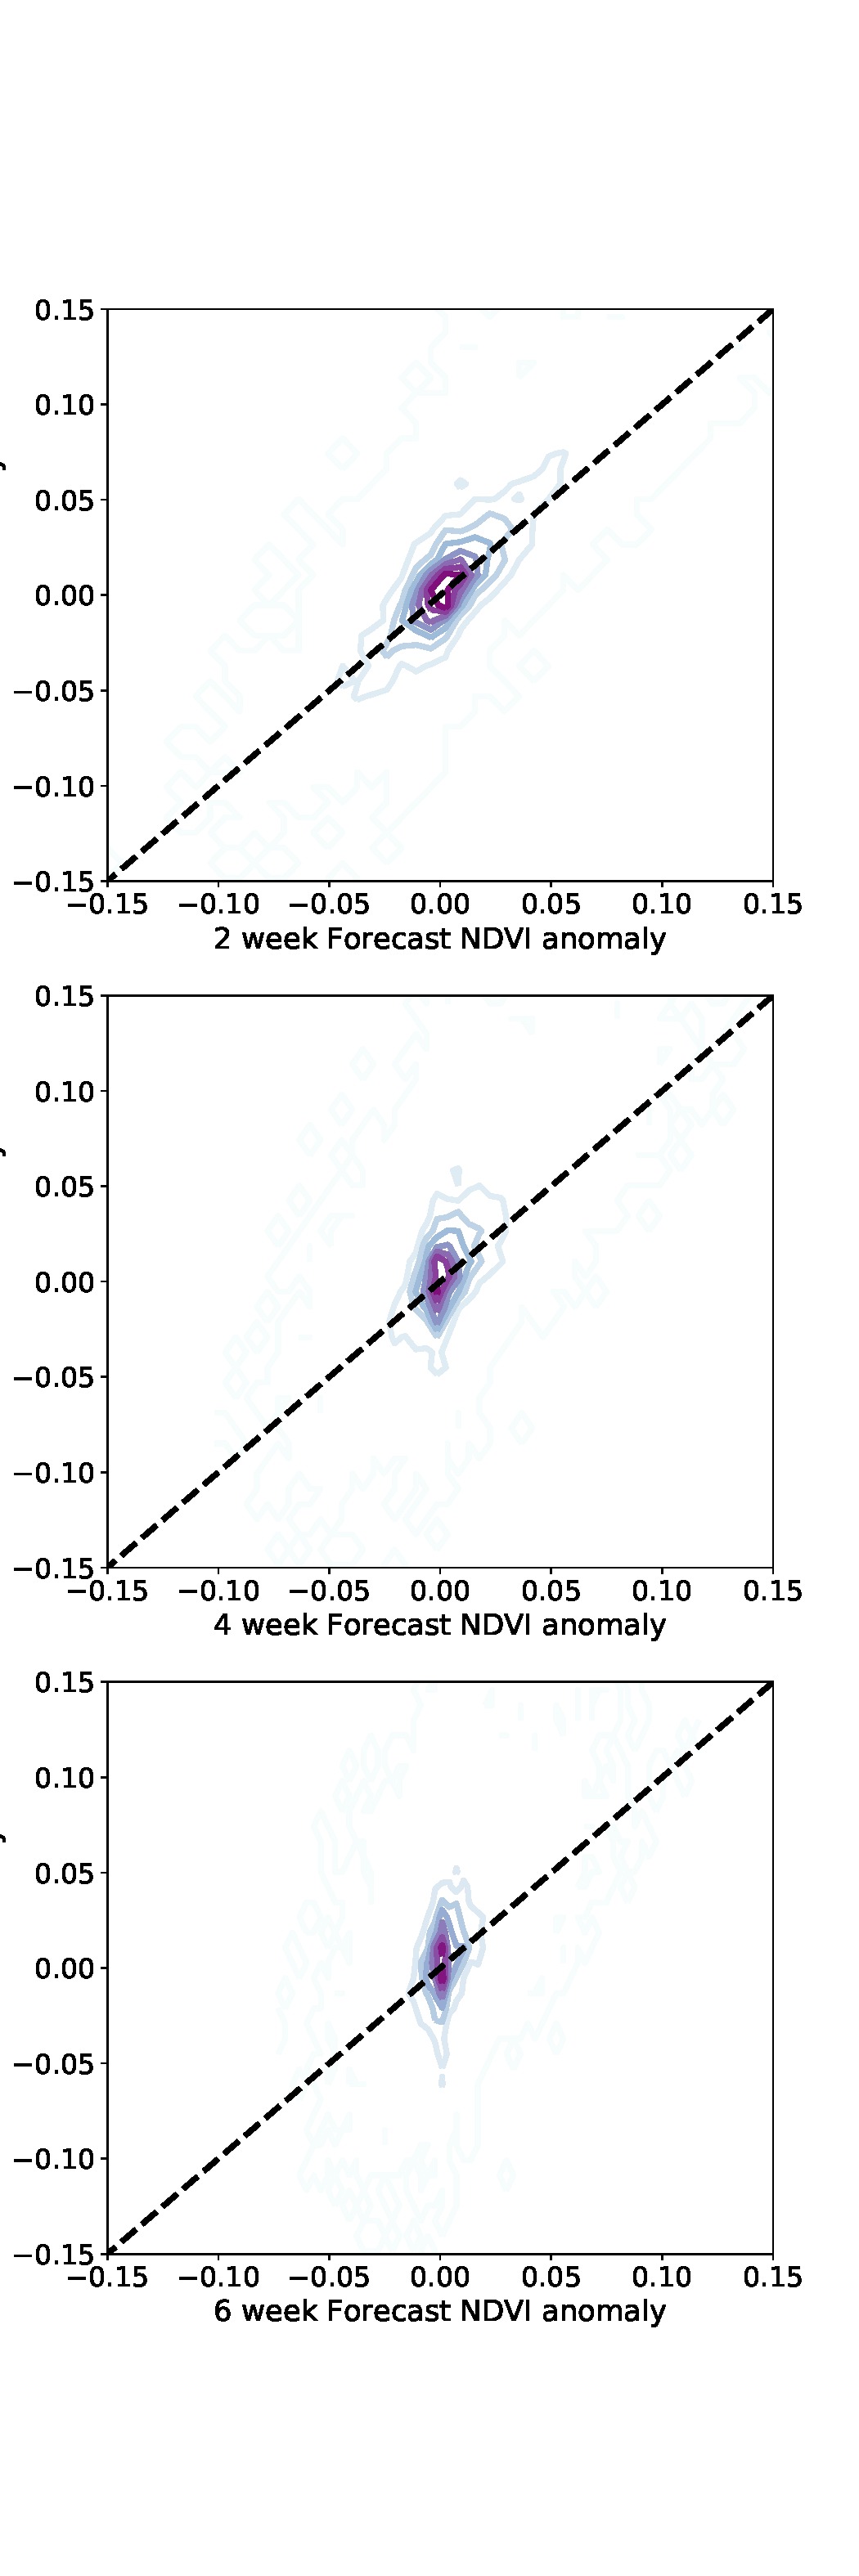
\includegraphics[trim = 30mm 35mm 0mm 10mm,width=5.4 cm]{figures/fig4left.pdf} \qquad 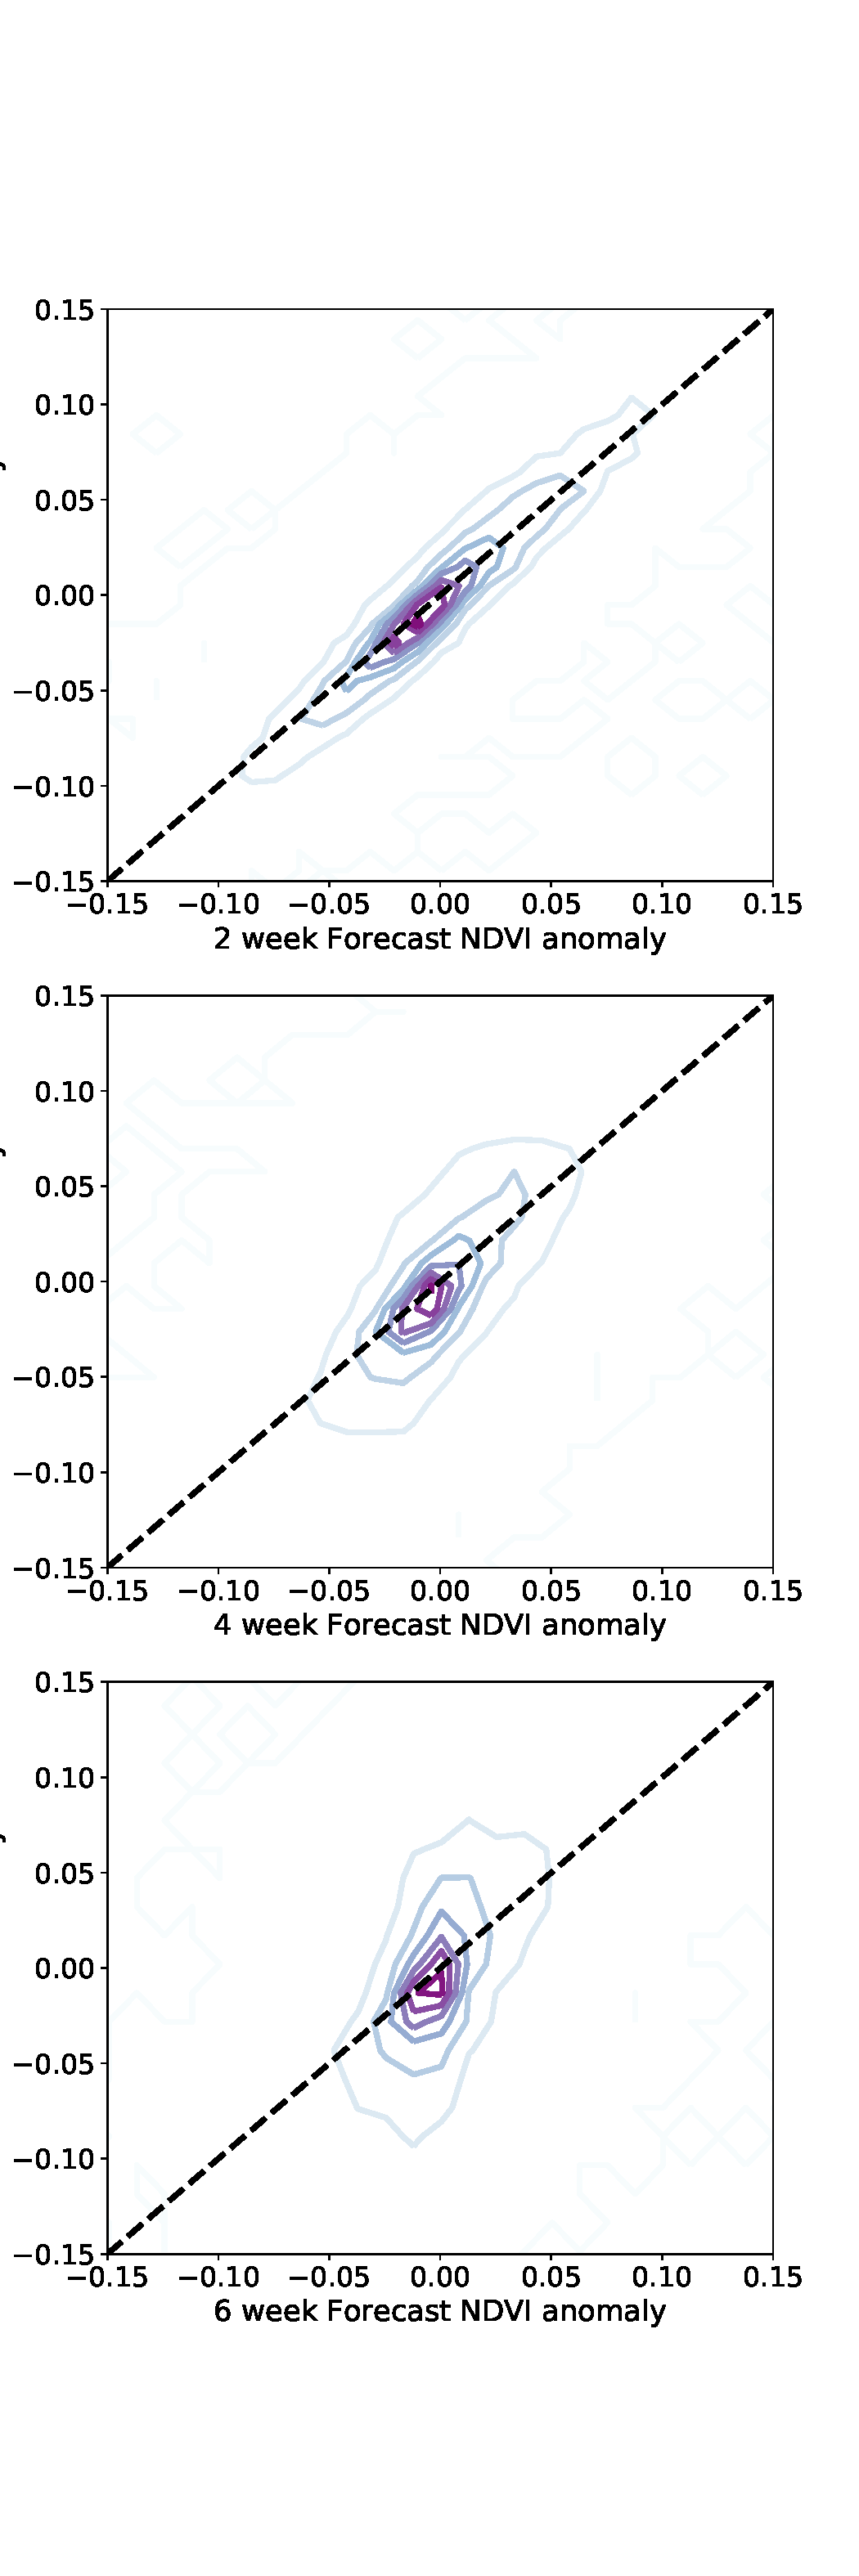
\includegraphics[trim = 0mm 35mm 30mm 10mm,width=5.4 cm]{figures/contour_adam_NDVI.pdf}
	\caption{\edit{TO DO: EDWARD, REFORMAT SO Y AXIS LABEL IS VISIBLE. Contour plots of NDVI anomaly against our two, four and six weeks NDVI anomaly forecast. The left three plots show our forecast performance for the GP method on Landsat data, and on the right the contours show the forecast performance for the AR method on MODIS data, across the 19 regions for which a forecast is possible more than 50\% of the time.}} \label{fig:contourNDVI}
\end{figure}


\begin{figure}
	\centering
	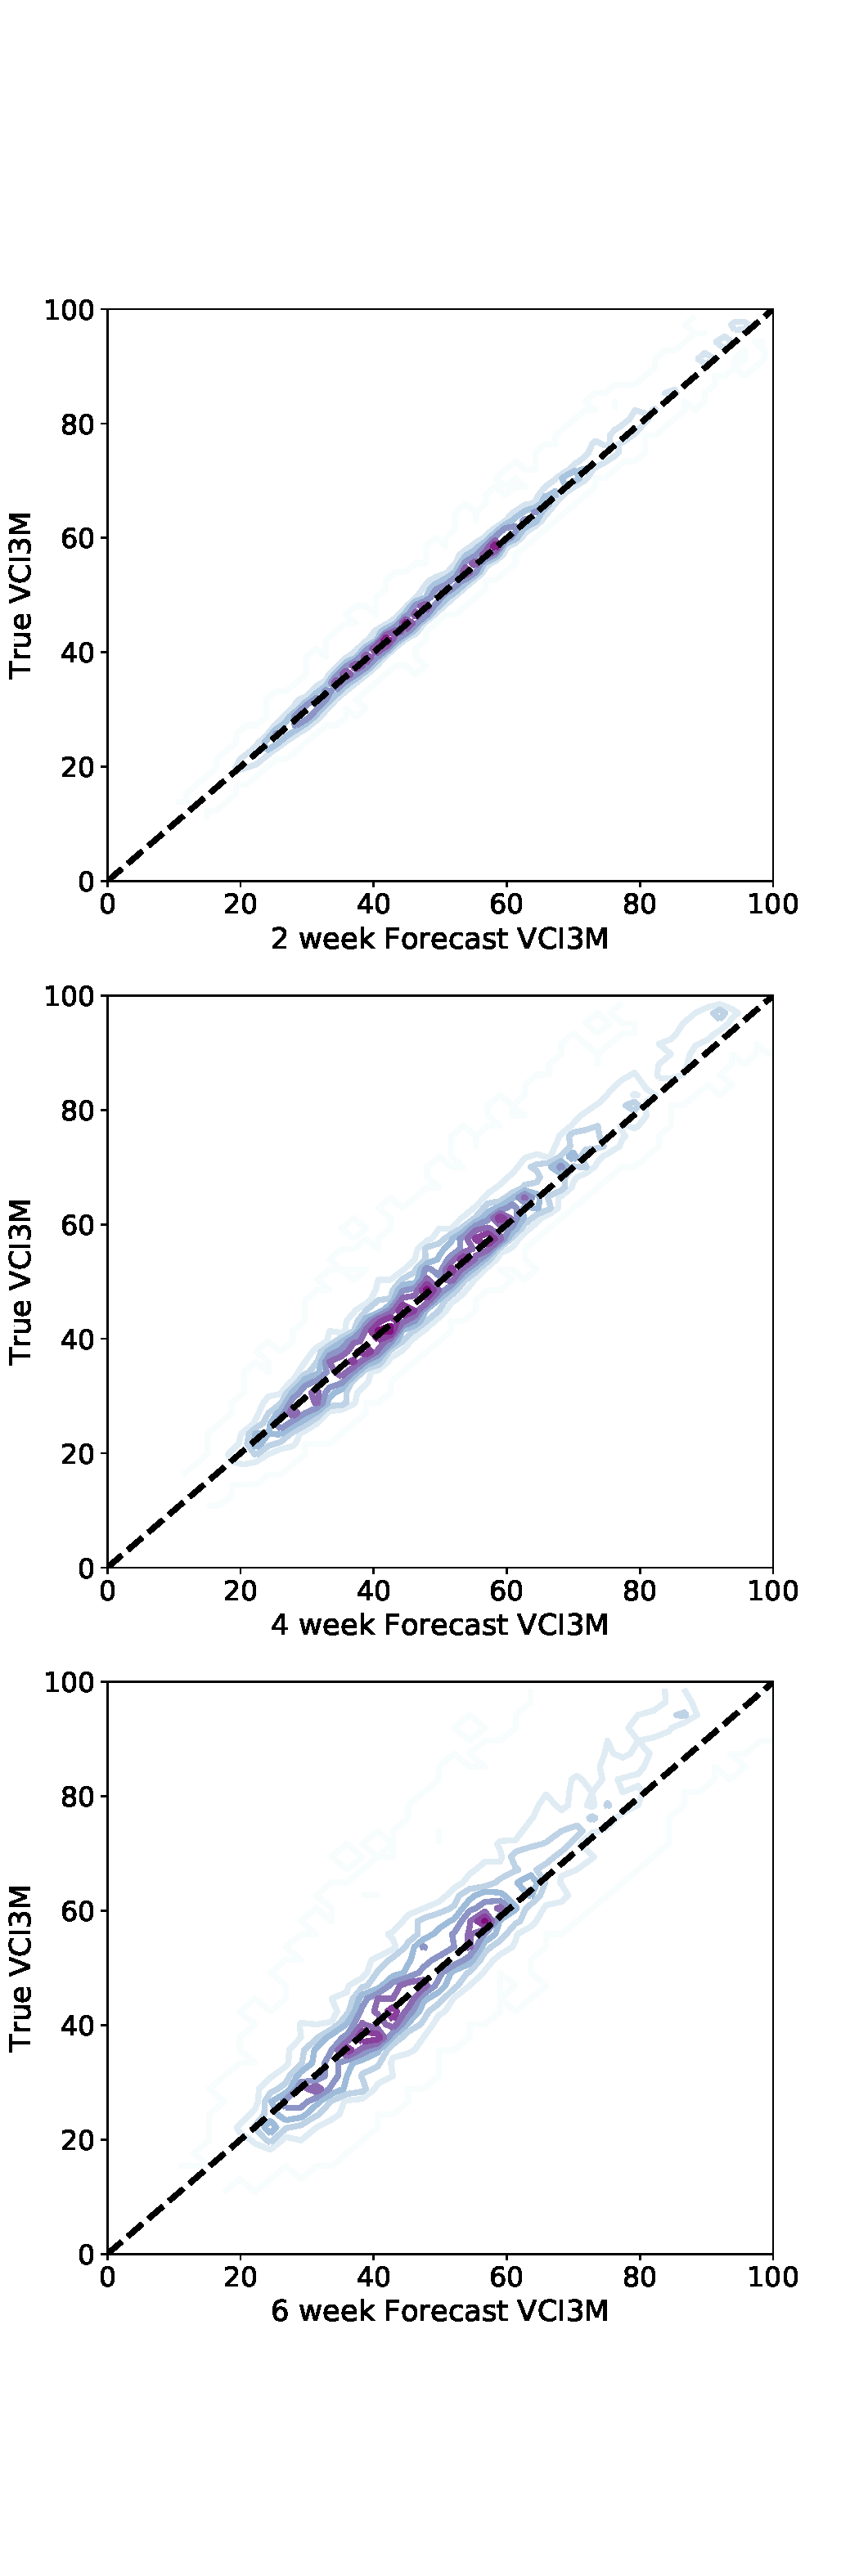
\includegraphics[trim = 30mm 35mm 0mm 10mm,width=5.4 cm]{figures/contour.pdf} \qquad 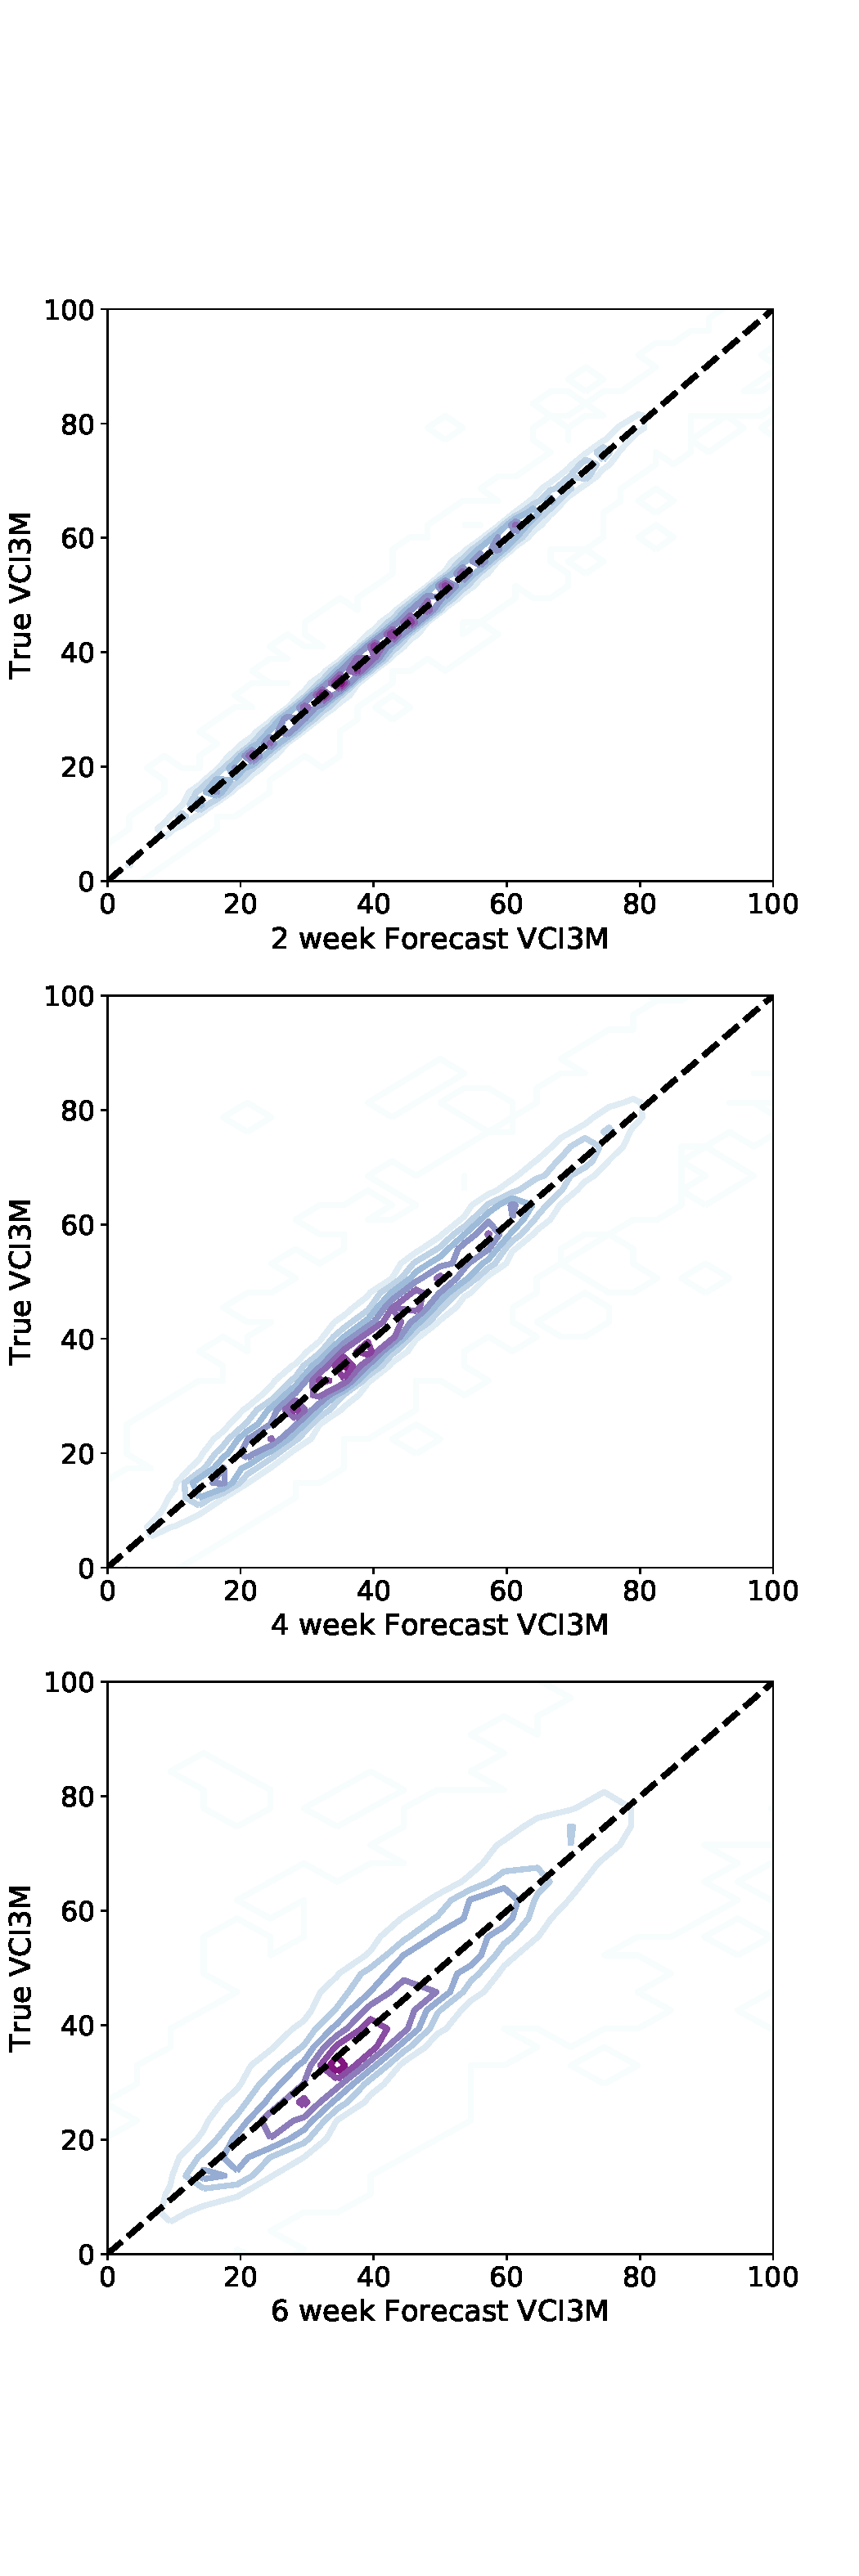
\includegraphics[trim = 0mm 35mm 30mm 10mm,width=5.4 cm]{figures/contour_adam.pdf}
	\caption{\edit{Contour plots of VCI3M against our two, four and six weeks VCI3m forecast. The left three plots show our forecast performance for the GP method on Landsat data, and on the right the contours show the forecast performance for the AR method on MODIS data, across the 19 regions for which a forecast is possible more than 50\% of the time.}} \label{fig:contour}
\end{figure}

\begin{table}
	\small
	\caption{\edit{TO DO: STEVEN/EDWARD FILL THIS OUT FOR GP/LANDSAT. Performance statistics of NDVI anomaly and VCI3m forecasting.}} \label{tab:stats}
	\centering
	\begin{tabular}{l|ccc|ccc} 
		\toprule
		& & \textbf{Landsat GP} & & &\textbf{MODIS AR} \\
		& \textbf{2 weeks} & \textbf{4 weeks} & \textbf{6 weeks} & \textbf{2 weeks} & \textbf{4 weeks} & \textbf{6 weeks} \\
		\midrule
		\textbf{NDVI anomaly:}&&&&&\\
		$R^2$-score  &  &  &  &0.85& 0.55& 0.33\\
		RMSE &  &  &  &0.025& 0.043& 0.053\\
		slope &  & & &0.99&0.99& 0.97\\
		intercept & & &&-0.00& -0.00& -0.00\\
		\midrule
		\textbf{VCI3M:}&&&&&\\
		$R^2$-score  &  &  &  &0.99& 0.96& 0.88\\
		RMSE &  &  &  &1.8& 4.3& 7.0 \\
		slope &  & & &1.00&1.00& 1.00\\
		intercept &  & &&-0.0& -0.1& -0.0\\
		\bottomrule
	\end{tabular}
\end{table}

\edit{The GP and AR forecasting methods were applied, on each of the two datasets, to regional aggregate NDVI and VCI3M time series. We focus on performance results of GP forecasting on Landsat data and AR forecasting on MODIS data since these two combinations of data and forecasting method performed the best (as measured by $R^2$-score, see Section \ref{app} in the Supplementary Material). Contour plots of forecast against actual data for two, four and six week forecasts are shown in Fig.~\ref{fig:contourNDVI} for NDVI anomaly, and Fig.~\ref{fig:contour} for VCI3M. Table \ref{tab:stats} shows the $R^2$-scores, RMSE, slope and intercept from each of these plots, and demonstrates that there is substantial forecast skill from each method at each lead time ($R^2$-scores are substantial), and that the forecasts are unbiased (slopes are all approximately 1, and intercepts approximately 0). The much higher $R^2$-scores for VCI3M compared to NDVI anomaly is explained by the fact that VCI3M is a 12 week aggregate, and hence its (near) future is actually derived from both past and future NDVI values.}

% Fig.~\ref{fig:timeline} shows that the same approximately linear relation between NDVI anomaly and lagged NDVI anomaly holds for the forecast and non-forecast mode time-series, and hence gives some validation of the method.\footnote{The assumption, under GP interpolation and extrapolation, that data anomalies follow a multivariate Gaussian distribution necessarily also assumes that the relationship between past and present anomalies are linear. This follows from the fact that a stationary Gaussian AR process must be linear \citep{Barrett:2010}.} Plots of NDVI anomaly against lagged NDVI anomaly showed that there is a strong linear relation between present and past observations of NDVI anomaly, see Fig.~\ref{fig:timeline}, thus it is anticipated that the linear AR model captures a good degree of the non-random relationship between past and future NDVI anomaly observations.

% \begin{figure}
% 	\centering
% 	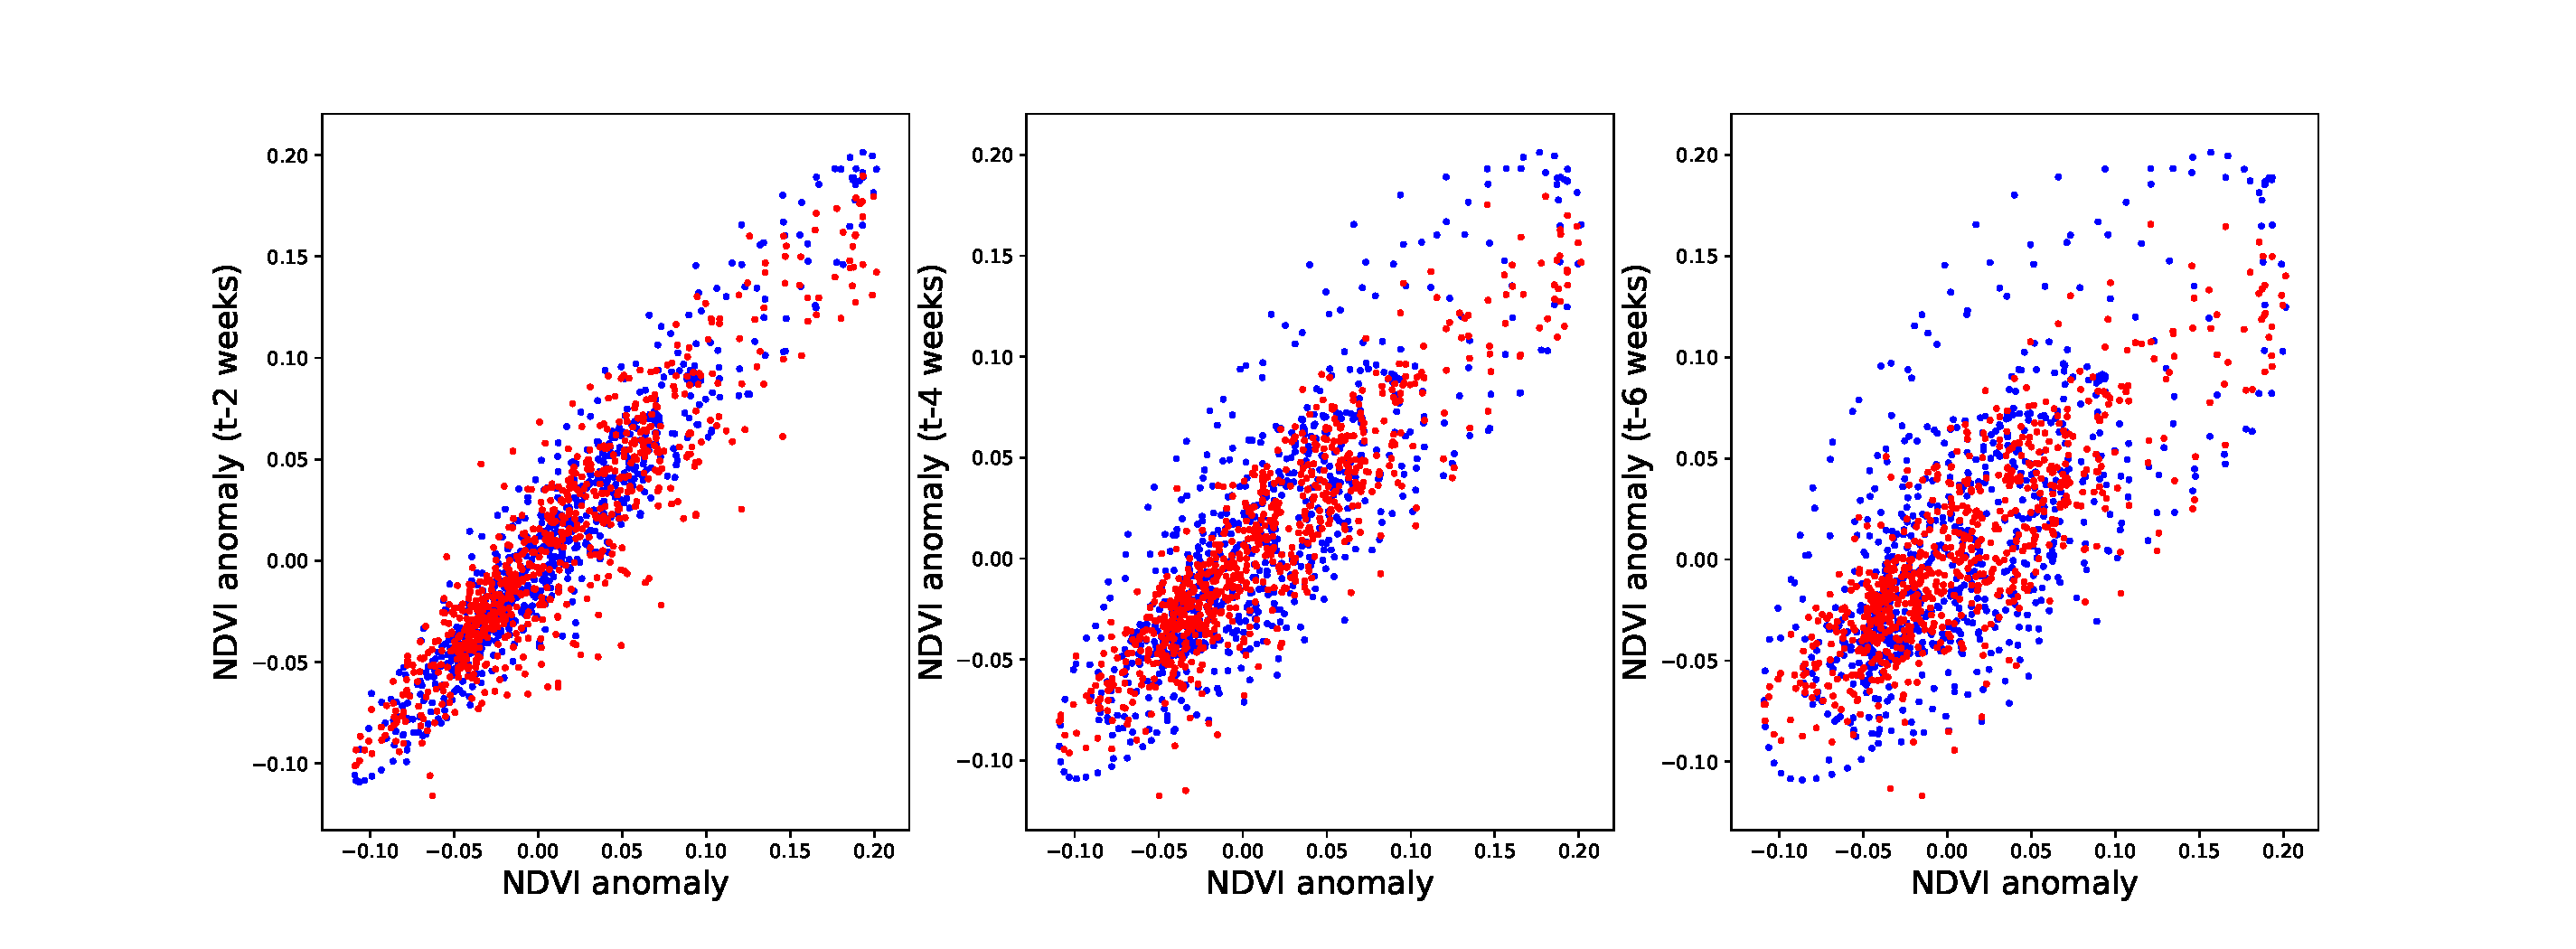
\includegraphics[trim = 50mm 4mm 0mm 3mm,width = 14 cm]{figures/timeline.pdf} 
% 	\caption{The approximately linear relation between Landsat NDVI anomaly and NDVI anomaly lagging at two, four and six weeks in the past. Blue dots show the Landsat data, processed with non-forecast mode GPs, which was taken as `ground truth'. Red dots show the data processed with forecast mode GPs, from which forecasts were generated.} \label{fig:timeline}
% \end{figure}

Due to the presence of non-interpolated gaps in the MODIS time series, there were weeks when a forecast assessment was not carried out on these data, see Section \ref{sec:Lmax} in the Supplementary Material for details.  For 15 of the regions, a 4 week forecast could be made on more than 90 percent of weeks; however, for some of the more cloudy/wet regions, a forecast could rarely be made, see Table \ref{tab:VCI3m_MODIS}.

\edit{To check if forecast skill depended on the true vegetation condition, RMS error was also computed separately for each of the five categories on the NDMA drought scale. The results are shown in Table \ref{tab:RMScategories}, where it can be seen that RMS error tended to be lower when there was a state of drought than when the vegetation condition was normal.} 

\begin{table}
	\small
	\caption{\edit{RMS error in VCI3M forecast, for the true vegetation condition belonging to the different categories of drought, at lead times of 2, 4 and 6 weeks. (The bottom category, extreme drought, did not occur according to the Landsat data.)} } \label{tab:RMScategories}
	\centering
	\begin{tabular}{l|ccc|ccc} 
		\toprule
		\textbf{Drought category} & & \textbf{Landsat GP} & & &\textbf{MODIS AR} \\
		& \textbf{2 weeks} & \textbf{4 weeks} & \textbf{6 weeks} & \textbf{2 weeks} & \textbf{4 weeks} & \textbf{6 weeks} \\
		\midrule
		Wet, VCI3M$>$50 & 2.2 & 5.3 & 9.0 &2.2& 4.8& 7.5\\
		Normal, 35$<$VCI3M$<$50 & 1.7 & 3.4 & 5.0 &1.6& 4.0& 6.5 \\
		Moderate drought, 20$<$VCI3M$<$35& 1.5 &3.2 & 5.0&1.5&3.7& 5.7\\
		Severe drought, 10$<$VCI3M$<$20& 1.1 &2.5 &5.5&1.4& 3.3& 5.4\\
		Extreme drought, VCI3M$<$10  & &&& 1.1 & 2.9   & 4.8         \\
		\bottomrule
	\end{tabular}
\end{table}

% \edit{Further graphs and tables are shown in the Supplementary Material, including: percentage standard deviation remaining for lead times of 1 to 10 weeks, see Fig.~\ref{fig:GP_NDVI_forecast} for GP forecasting on Landsat data and Fig.~\ref{fig:NDVI_forecast} for AR forecasting on MODIS data; the $R^2$-score and reduction in standard deviation for the two, four and six weeks forecasts for each individual region, see Tables \ref{tab:NDVI_LS} to \ref{tab:NDVI_MODIS}; tables of results of NDVI forecasting with the other dataset/method combinations, see Table \ref{tab:NDVI_GPM} for GP forecasting on MODIS data and Table \ref{tab:NDVI_Landsat_AR} for AR forecasting on Landsat data.}

\edit{To check if forecast skill depended on the time of year, RMS error of VCI3M forecast was plotted against the week of the year, see Fig.~\ref{fig:seasonal}. The plot shows that the seasonal differences in RMS error are not substantial on the scale on which VCI3M varies, although RMS error was generally somewhat elevated for some of the January/February dry season.}

\begin{figure}
	\centering
	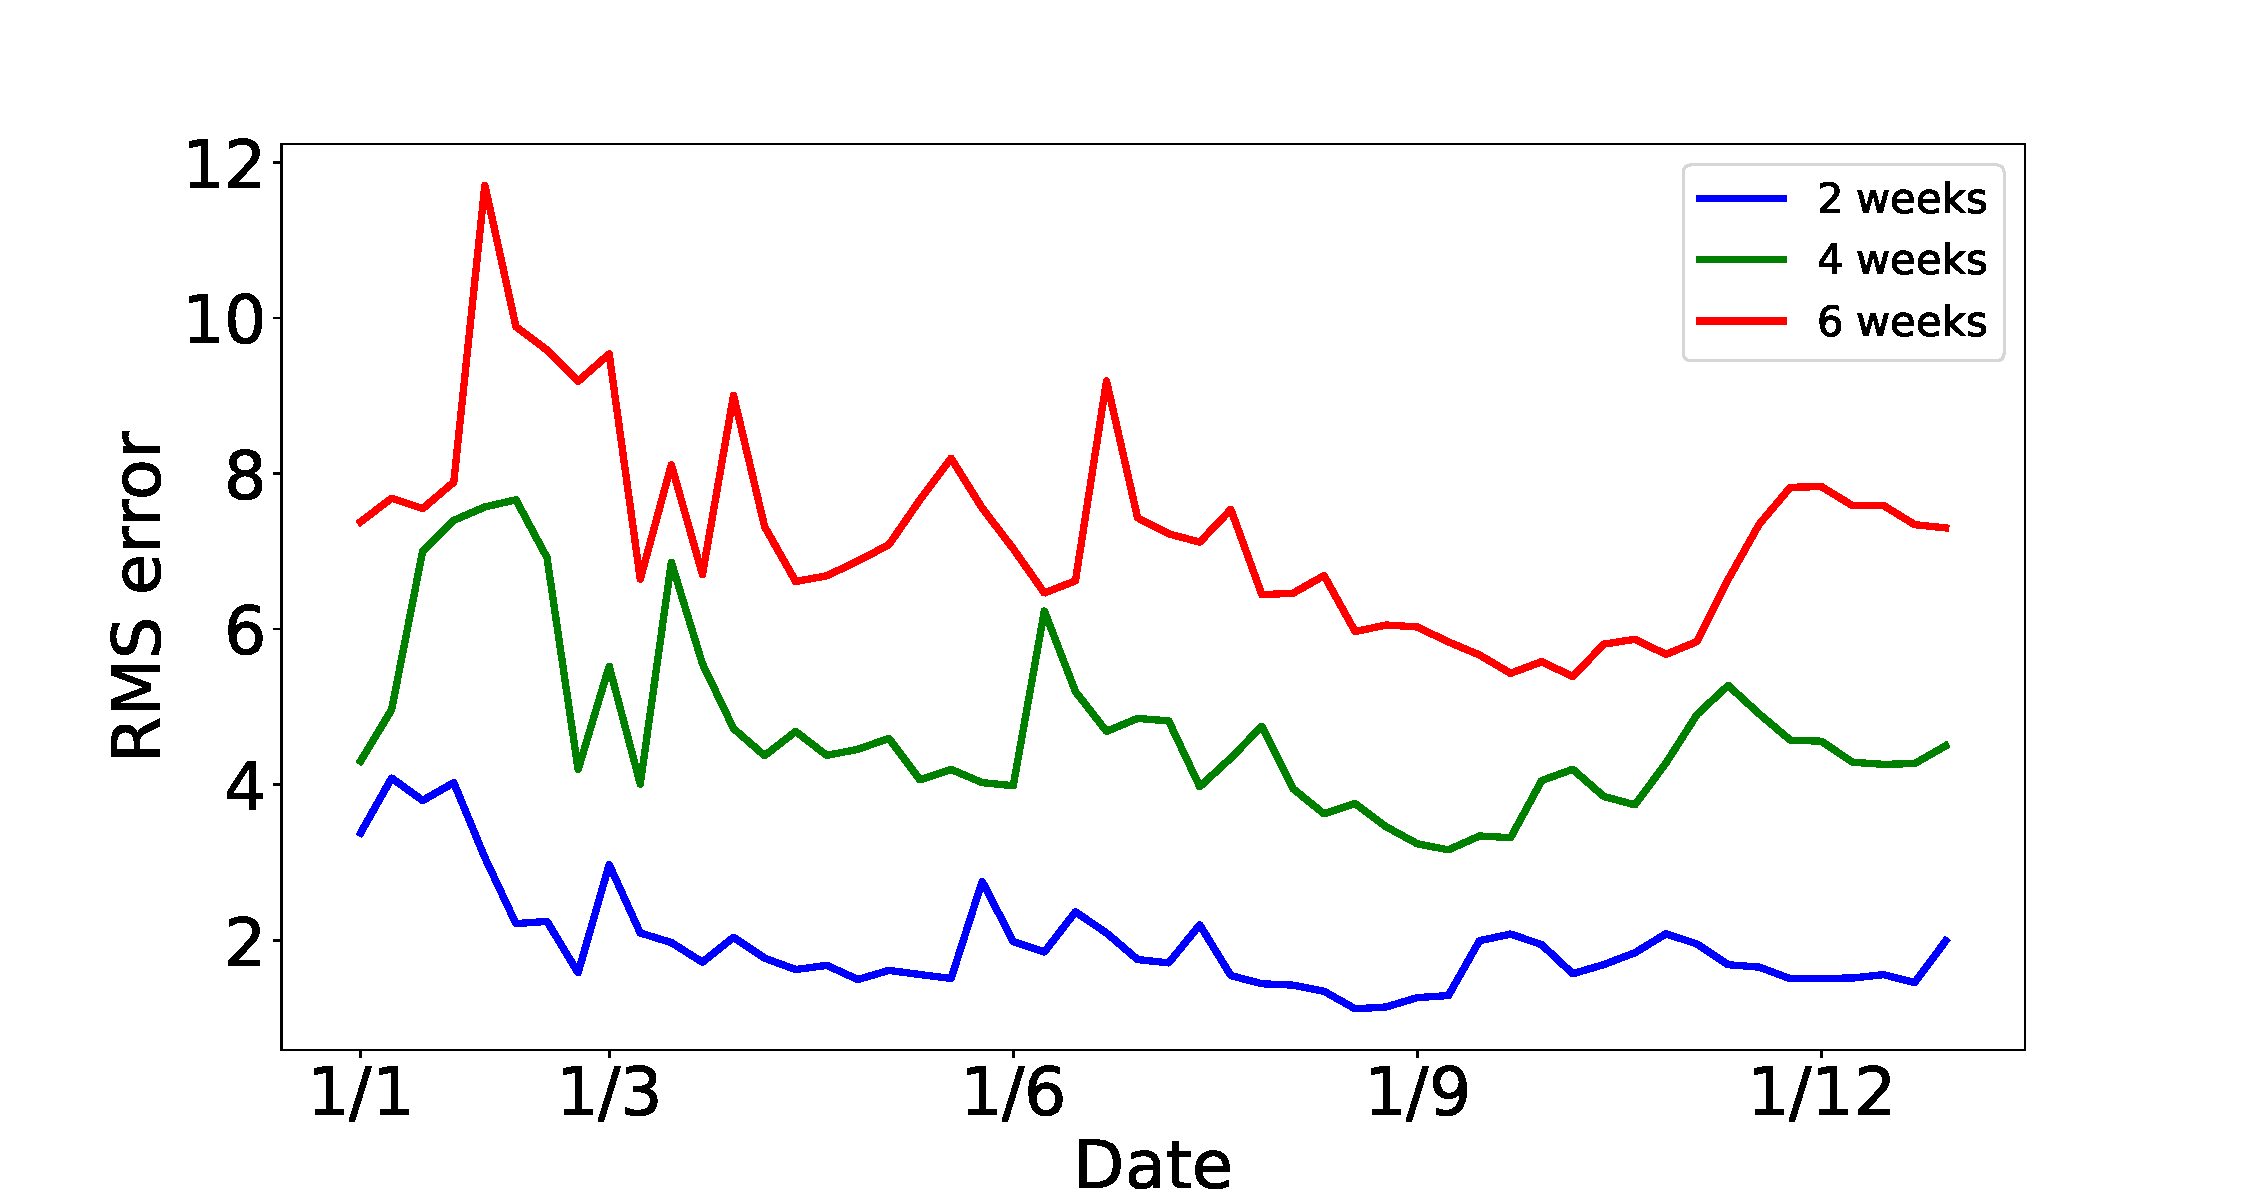
\includegraphics[trim = 30mm 35mm 0mm 10mm,width=5.4 cm]{figures/seasonal_MODIS.pdf} \qquad 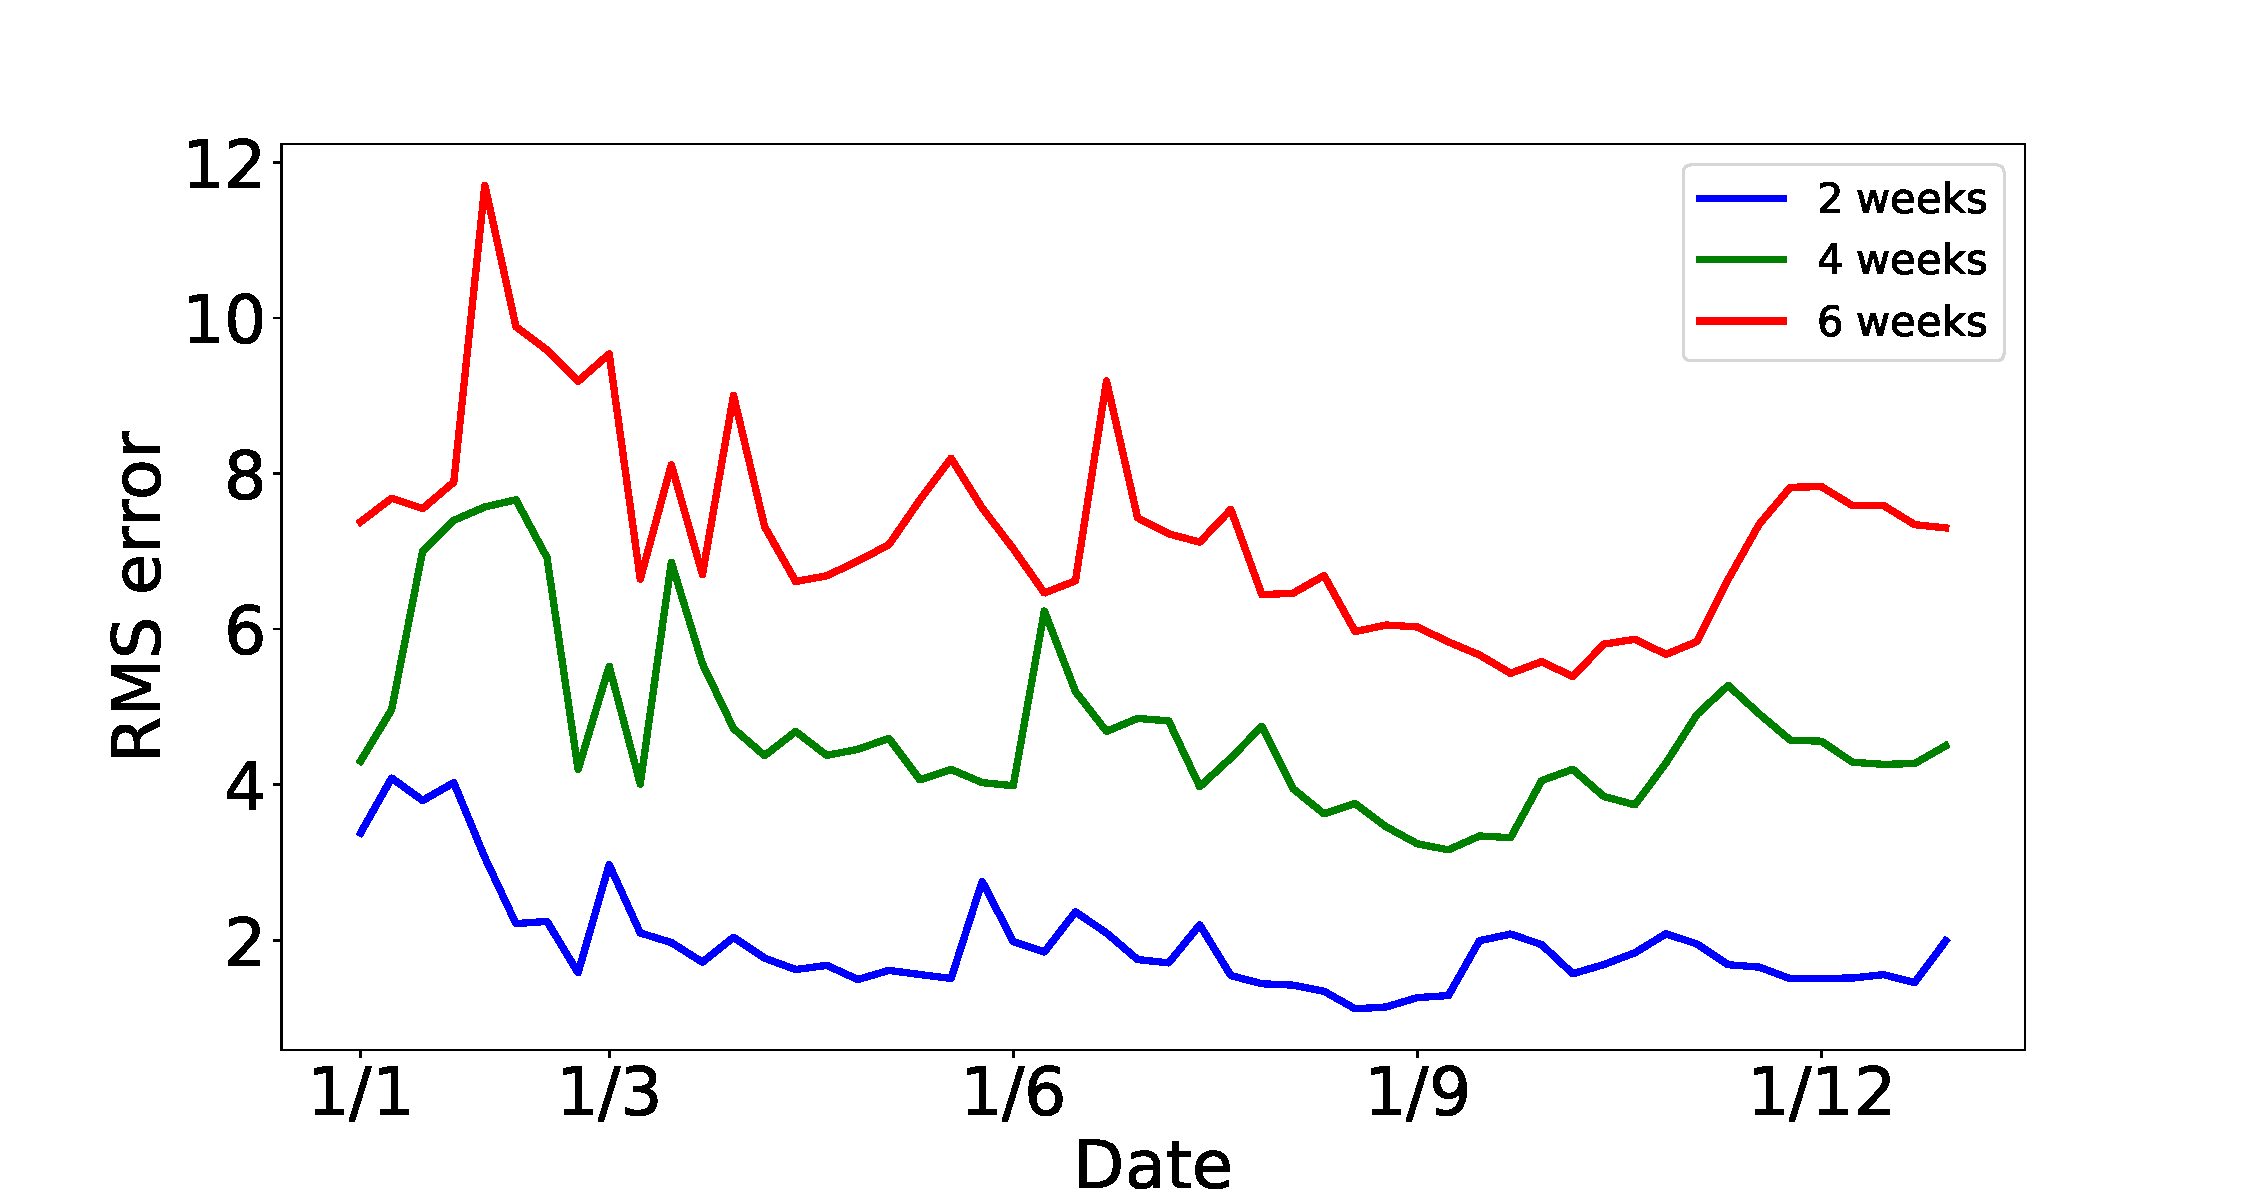
\includegraphics[trim = 0mm 35mm 30mm 10mm,width=5.4 cm]{figures/seasonal_MODIS.pdf}
	\vspace{0.5cm}
	\caption{\edit{TO DO: STEVEN/EDWARD REPLACE LEFT HAND PLOTS WITH THE CORRESPONDING PLOTS FROM LANDSAT/GP. RMS error of VCI3M forecast for each week of the year. (Left) GP forecasting on Landsat data. (Right) AR forecasting on MODIS data.}} \label{fig:seasonal}
\end{figure}



\subsection{Drought event forecast: ROC curves}



\begin{figure}%
	\centering
	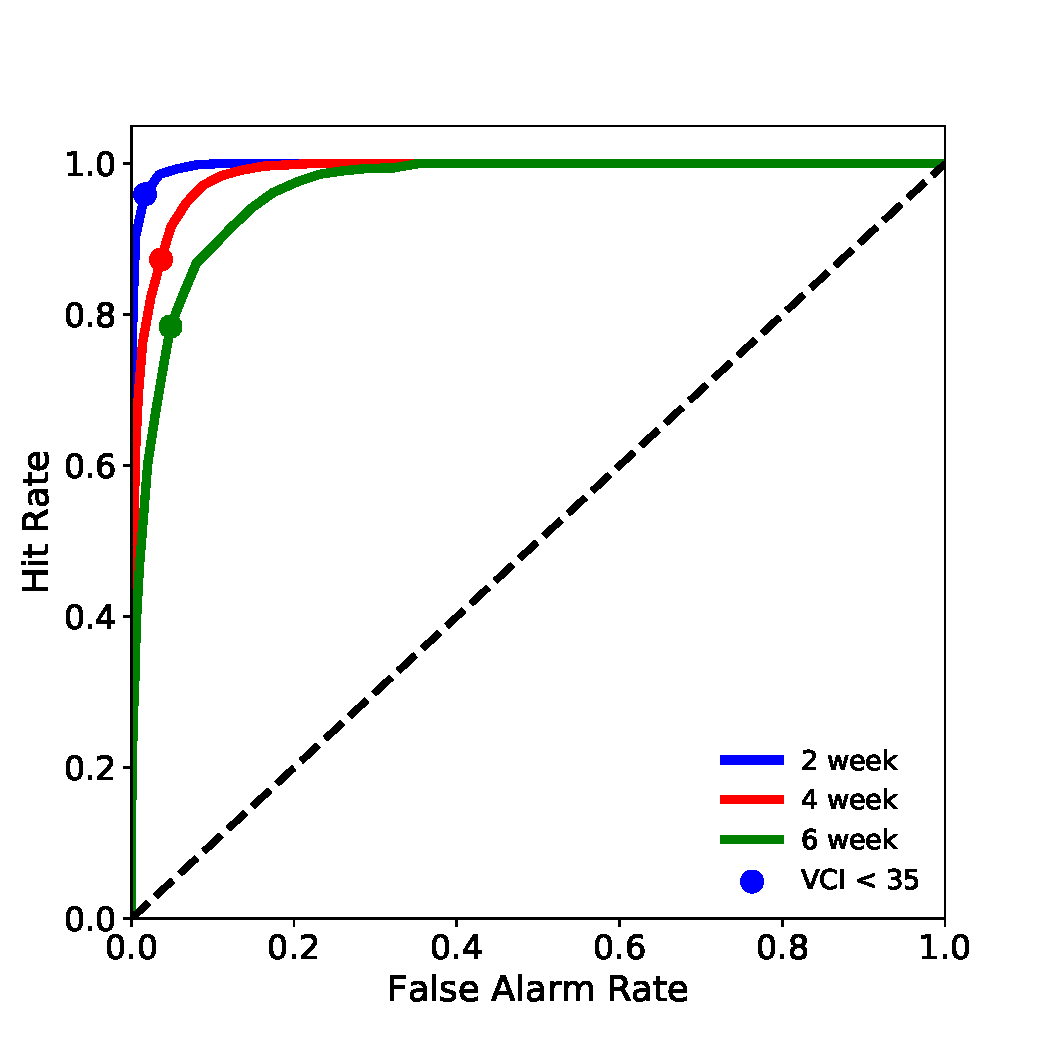
\includegraphics[trim = 20mm 4mm 12mm 3mm,width=5.6 cm]{figures/VCIfcO.pdf}
	\qquad
	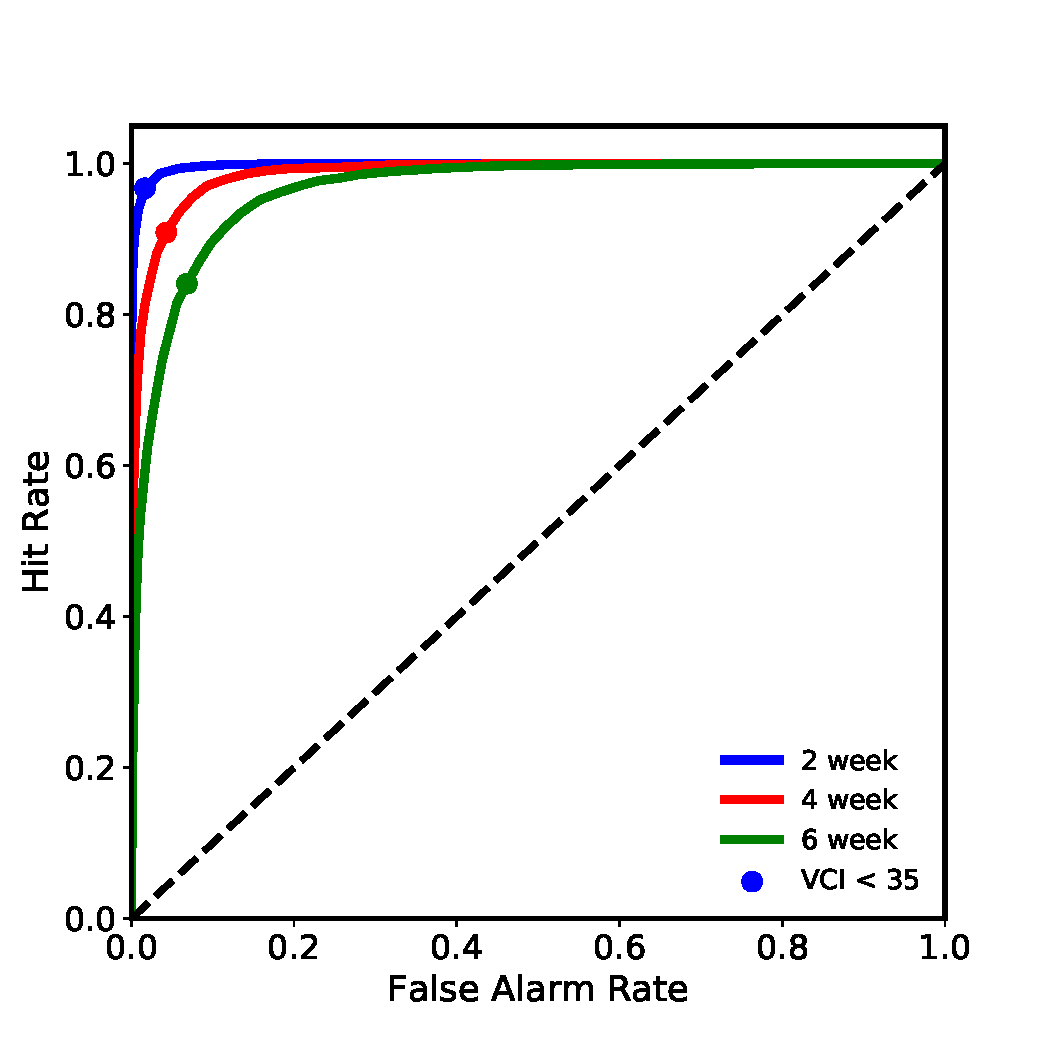
\includegraphics[trim = 12mm 4mm 20mm 3mm,width=5.6 cm]{figures/VCIfc0abb2.pdf}
	\caption{(Left) ROC curve for drought detection (VCI3M $<$ 35) for lead times of 2, 4 and 6 weeks using the GP method. (Right) ROC curve for drought detection using the AR method. The curves are plotted from applying different thresholds to convert the continuous forecast into a binary forecast of drought or no drought, see text for details. The shaded circles show the point obtained from forecasting drought when the predicted VCI3M$<$35. The area under the curve is 1.0, 0.98, 0.96 (GP, left) and 1.0, 0.99 and 0.96 (AR, right) for lead times of two, four and six weeks, respectively. }
	\label{fig:ROC_abb}
\end{figure}





To assess the usefulness of the AR and GP methods for drought forecasting, we tested their ability to detect specific drought events, as defined by the NDMA's alert threshold \citep[VCI3M$<$35,][]{rs8040267}. Receiver operating characteristic (ROC) curves were plotted for detection of VCI3M$<$35 at lead times of two, four and six weeks (Fig.~\ref{fig:ROC_abb}). These curves show the probability of predicting a state of drought (VCI3M$<$35) when there will be a state of drought, i.e.~hit rate, against the probability of predicting drought when there will not be drought, i.e.~false alarm rate, for varying binarisation thresholds on the forecast. These curves give an indication that one can forecast droughts with these methods even as far as six weeks ahead. 

The ROC curve performance is not highly dependent on the region (see Table \ref{tab:ROC2}). Even for the wetter Eastern regions, for which observations are sparser due to cloud cover, the hit and false alarm rates only differ by 1 to 2 percentage points compared with those computed across all regions. \edit{Further, ROC curves for predicting the NDMA drought categories of severe} (10$<$VCI3M$<$20) or extreme (VCI$<$10) drought look similar to those for detecting VCI3m$<$35, \edit{see Fig.~\ref{fig:ROCotherdrought}.}  Together, these results demonstrate that there is a huge potential for drought forecasting, and encourage a future cost-benefit analysis of applying such a forecast in practice.



\begin{table}
	\small
	\caption{False alarm rate and hit rate (respectively, in percent) for different regions in Kenya based on forecasting drought if the predicted VCI3M is less than 35.} \label{tab:ROC2}
	\centering
	\begin{tabular}{l|ccc|ccc} 
		\toprule
		\textbf{Regions} & & \textbf{Landsat GP} & & &\textbf{MODIS AR} \\
		& \textbf{2 weeks} & \textbf{4 weeks} & \textbf{6 weeks} & \textbf{2 weeks} & \textbf{4 weeks} & \textbf{6 weeks} \\
		\midrule
		All & 2\% \; 96\% & 4\% \; 87\% & 5\% \; 78\% & 2\% \; 97\% & 4\% \; 91\% & \; 7\% \; 84\%\\
		Z24 & 2\% \; 99\% & 4\% \; 91\% & 5\%  \; 82\% & 2\% \; 98\% & 5\% \; 94\% & \; 8\%  \; 88\%\\
		North (Z1,3 and 5) & 1\% \; 97\% & 2\% \; 88\% & 3\%  \; 76\% & 2\% \; 98\% & 6\% \; 93\% & 11\% \; 87\%\\
		East (Z7, 9, 10 and 11) & 3\% \; 94\% & 5\% \; 85\% & 6\% \; 77\% & 3\% \; 97\% & 6\% \; 91\% & 10\% \; 85\%\\
		South (Z15 and 18)  & 1\% \; 96\% & 3\% \; 88\% & 4\% \; 77\% & 2\% \; 98\% & 6\% \; 94\% & 11\% \; 90\%\\
		\bottomrule
	\end{tabular}
\end{table}

 



%%%%%%%%%%%%%%%%%%%%%%%%%%%%%%%%%%%%%%%%%%
\section{Discussion and Conclusion} \label{sec:dis}

This paper highlights the potential of two separate methods for drought forecasting in pastoral regions of Kenya. The linear autoregression models applied to MODIS achieved an $R^2$-score of 0.58 for NDVI anomaly at a lead time of 4 weeks, and an $R^2$-score of 0.95 for the VCI3M, the three-month vegetation condition index used within the drought early warning system developed by the National Drought Management Authority. The Gaussian Processes method was applied to Landsat and achieved an $R^2$-score of 0.36 for NDVI anomaly at a lead time of 4 weeks, and an $R^2$-score of 0.94 for the VCI3M. Importantly, both methods showed high sensitivity and specificity for prediction of VCI values indicative of drought, at lead times of 2, 4 and 6 weeks (see Fig.~\ref{fig:ROC_abb}). We have presented results at the level of livelihood zone and county intersections, however both methods can be applied at any suitable spatial unit (e.g., grazing units) due to the high spatial resolution of both satellite datasets.


Both methods constitute novel analyses of vegetation index time series. To our knowledge, this is the first time that the GP method for NDVI forecasting has been applied to large amounts of real data and used for gap-filling. We have shown that GPs are a very useful addition to other methods for both these purposes. Similarly, linear AR of NDVI, or of Granger causality of various variables to NDVI, has not previously been explored at a temporal resolution as fine as 1 week. That such substantial $R^2$-scores can be achieved for NDVI anomaly at a lead-time of several weeks just by using the past few observations of NDVI anomaly in a linear AR model is a novel finding. Furthermore we moved beyond fitting a single model, and rather fit models to segments of data, repeatedly using refreshed models to forecast subsequent observations not used in the model fitting (i.e.~we had separation of training and testing models). 



Droughts  have many adverse effects on pastoral and agro-pastoral communities as they mainly rely on rainfall for food and fodder availability. In order to reduce drought-related damage and losses within these communities, local, national, and international stakeholders often decide to act on information provided by EWS which may come too late \citep{tand}. Indeed, these systems tend to monitor current, rather than forecast future, environmental and socio-economic factors in a region, and sound the alarm when the situation is already critical. Some EWS now include a qualitative assessment of future rainfall. However, a meteorological or hydrological drought will not necessarily lead to agricultural damage \citep{BHUIYAN2006289}. To mitigate the impacts on food security and nutrition, EWS need to focus on monitoring and forecasting the possible socio-economic impacts of future rainfall variability on agricultural drought \citep{wmo2015wmo}. Additionally, acting ahead of a disaster instead of providing humanitarian assistance once a disaster hits can save money and lives \citep{venton2012economics}. The methods developed in this study allow disaster risk managers to estimate vegetation condition to access resources and limit the impacts for pastoralist communities up to six weeks ahead. For example, in Kenya, the emergency funds that are linked to the VCI could be accessed earlier to launch livestock destocking and vaccination campaigns. Future work should focus on methods that forecast socio-economic drought indicators such as livestock mortality, milk production, or food prices. 

Droughts are complex and hence inherently difficult to define and measure \citep{MISHRA2010202}. A large number of satellite-based indicators have been developed to identify meteorological, hydrological, and agricultural droughts \citep{zargar2011review,aghakouchak2015remote} with each performing well in space and time to a certain degree \citep{ZHANG201796}. While its limitations are known, the VCI used in this study has been introduced as one of the main biophysical indicators in the drought early warning system operated by the NDMA, with specific thresholds to identify different levels of drought throughout the ASAL regions of Kenya \citep{rs8040267}. In future, we suggest that the performance of this indicator together with the thresholds used should be linked to ground-based measurements over various agro-ecological zones.



Droughts have devastating impacts on many people around the world. There are increasing efforts to develop tools and identify actions to save lives and livelihoods before these disasters strike. The methods developed in this study can help policy makers, disaster risk managers and other key stakeholders to understand up to six weeks in advance the state of vegetation in pastoral areas. This will allow them to access resources and develop procedures before the impacts of drought become visible to mitigate the adverse effects in these vulnerable communities. To further strengthen EWS, future research needs to clearly identify satellite-based indicators and thresholds of drought (which may vary in time and space), to build a relation between observable indices and future impacts. More work is also needed to understand how a hazard (e.g., reduced rainfall) becomes a disaster (e.g., food insecurity) so that these events can be better forecasted.




\section*{Authors responsibilities}
A.B.B., S.D. and E.S. are lead authors as they contributed equally to the paper and the order of the three names is alphabetical. A.B.B was responsible for the Linear AR and Granger causality calculations, and the text describing those methods. S.D. was responsible for the GPs used in the paper and was responsible for the usage of all the Landsat data and the text describing those methods. E.S. was responsible for the MODIS data accumulation, creation of the MODIS time series and the filtering of the MODIS data and the text describing those methods. SO and PR developed the initial idea and provided feedback throughout. All authors wrote, reviewed and edited the final manuscript. We acknowledge early contributions to pilot work from Peter Hurley, Philip Rooney, Martin Jung, and J\"{o}rn Scharlemann.

\section*{Acknowledgements}
This research was funded by the STFC through the following projects: ``AstroCast: Applying Astronomy Data Analysis to enhance disaster forecasting'' -- grant number ST/R004811/1; and ``STFC Official Development Assistance (ODA) Institutional Award" attached to the same grant and; "A UK-Africa Data Science Network: Capturing the SKA-Driven Data Transformation'' grant number ST/R001898/1. This project was initiated through pump-priming funding from the University of Sussex's ``Sussex Research" thematic programme and carried out as part of the interdisciplinary Data Intensive Science Centre at the University of Sussex (DISCUS)






%\appendixtitles{no} %Leave argument "no" if all appendix headings stay EMPTY (then no dot is printed after "Appendix A"). If the appendix sections contain a heading then change the argument to "yes".
%\appendixsections{one} %Leave argument "multiple" if there are multiple sections. Then a counter is printed ("Appendix A"). If there is only one appendix section then change the argument to "one" and no counter is printed ("Appendix").

\appendix

\section{Comparison of the two datasets}
The key differences between the two datasets are the spatial and temporal resolutions, see Table \ref{tab:comp}. The Landsat data had higher spatial resolution, whilst the MODIS data had higher temporal resolution. Since forecasting was being attempted at the level of large scale regions (livelihood zone and county intersections), and at a weekly temporal resolution, the expectation was that the MODIS data would have advantages,  assuming individual Landsat and MODIS observations have similar signal-to-noise ratios. The processed MODIS time series with weekly observations have less measurement noise because they are composites of 7 daily observations \edit{(that themselves are 16-day composites of measurements taken every 1-2 days)}, whereas the processed Landsat time series are derived from more temporally sparse data (up to 3 different Landsat missions, each yielding one observation every 16 days). Landsat data would have advantages in different applications where forecasts on smaller spatial scales are required. The Landsat data also has the advantage that the quality flags and cloud masks are defined on smaller scales.    



\begin{table}
	\small
	\caption{Table comparing Landsat and MODIS products}
	\label{tab:comp}
	\centering
	\begin{tabular}{lccc}
		\toprule
		\textbf{Feature}	& \textbf{Landsat} & \textbf{MODIS}\\
		\midrule
		\textbf{Spatial Resolution} & 	High resolution at 30\,m 	&   Medium resolution ranging from 250\,m to 1\,km \\
		\textbf{Temporal Resolution}	&  16-day sampling (8-day when	&   Daily sampling    \\ 
		&  both Landsat-7 and 8 are used) & monitoring dynamic variables \\
		\textbf{Quality} &Cloud coverage at 30\,m & Cloud coverage at 500\,m \\
		
		\bottomrule
	\end{tabular}
\end{table}

The differences between the MODIS and Landsat datasets produced slightly different “True” aggregate time series on which to assess the interpolation and forecasting methods. In addition to the different temporal resolution of the observations supplying the final time series, the MODIS data were aggregated across 100 random grassland pixels from each region, whereas the 1\,000 Landsat pixels analysed were randomly distributed over the whole of each region. \edit{In choosing how many pixels to analyse per region, there is a trade-off between using a larger number of pixels for higher accuracy, and a smaller number of pixels for lower computational cost. Fewer MODIS pixels were used than Landsat pixels since they correspond to larger spatial regions. Both these choices of number of pixels should be sufficient for high accuracy of results, since for Landsat data the $R^2$-score comparing the average of all pixels from a region with the average of 100 or 1\,000 random pixels was 0.990 and 0.9993 respectively.} The MODIS grassland classification was not available at Landsat resolution, thus unambiguous classification of the smaller Landsat pixels was not possible. This is unlikely to have made much difference to pixel selection, given that the pastoral livelihood zones are mostly grasslands (Fig. \ref{fig:l_zone}). 

\section{Further details on methods}

% Interpolation of gaps was vital for accurate construction of NDVI anomaly and VCI from raw NDVI, since calculation of these requires the raw NDVI values for the corresponding week in every year of the recording, see Section \ref{sec:vci}. Further, for AR forecasting (Section \ref{sec:ARmethod}), lengthy segments of regular gridded data must be input for good model parameter estimation. 

\subsection{Gaussian process modelling} \label{sec:GPM}
A Gaussian Process is a probabilistic model defined as a collection of random variables for which any finite subset has a joint Gaussian distribution \citep{gpm}. Formally, for an output $y$ and inputs $\textbf{x}$:
\begin{align}
	f(\textbf{x}) &\sim \mathcal{GP}(m(\textbf{x}), k(\textbf{x},\textbf{x'})),\\
	y_i &= f(\textbf{x}_i) + \sigma_r,
\end{align}
where the mean function $m(\textbf{x})$ represents the expectation $E[f(\textbf{x})]$ and the kernel function $k(\textbf{x}, \textbf{x'})$ defines the covariances ${\rm cov}(f(\textbf{x}), f(\textbf{x'}))$, which specifies how similar outputs $f(x)$ and $f(x^\prime)$ are. The sample drawn from $f(\textbf{x})$ at locations ${\textbf{x}}_{n=1}^N$ follow a joint multivariate Gaussian distribution with covariance matrix determined by the kernel function. Here, the $\textbf{x}_i$ are the dates, $t_i$, of the observations, and $y_i$ is the NDVI at time $t_i$, subject to measurement error $\sigma_r$. To interpolate, the existing data were used to fit the mean $m$ and the kernel $k$, and then the GP with the fitted mean and kernel provided an estimate of the probability distribution for the missing data.

\edit{The mean $m(t)$ was set to be constantly the mean of the whole time series.} To determine the kernel, compositional Kernel Search \citep{pmlr-v28-duvenaud13} was used to determine the best kernel combination, by calculating the maximum evidence\footnote{In practice the evidence lower bound (ELBO) was used instead of the evidence ($p_\sigma$) with $\log(p_\sigma) \ge$ ELBO} (Marginal likelihood) for any product or sum of two common kernel combinations (Linear,  Radial Basis Function, Periodic, Rational Quadratic and Matern). The kernel with the highest evidence for the Landsat NDVI time series was the Radial Basis Function (RBF) in addition to the Periodic kernel ($k_{RBF}+k_P $), where the period $p$ was set to one year:
\begin{align}
	k_{RBF}(t,t') &= \sigma_{RBF}^2 \exp{\Big( -0.5 \frac{|t-t'|^2}{l_{RBF}^2} \Big) }, \label{eq:eqr} \\
	k_P(t,t') &=    \sigma_{P}^2 \exp{\Big(-2 \frac{\sin^2(\pi |t-t'|/p)}{l_{P}^2}\Big)}. \label{eq:eqP}
\end{align}
This GP contains 5 parameters to be fit ($\sigma_r$, $\sigma_{RBF}$, $l_{RBF}$, $\sigma_{P}$, $l_{P}$), which were learned using Stochastic Variational Inference (SVI). The code was written using the Deep Universal Probabilistic Programming language from \texttt{Pyro}, which is written in \texttt{Python} and supported by \texttt{PyTorch}. 

\edit{Gridding and gap-filling on Landsat data was carried out by fitting the above-described GP model to individual pixel time series, and then using the model to output an expected NDVI value every Saturday from 1/1/2000 until 2/2/2019. Note that} the processed, gap-filled, time series have distinct observation dates from the raw data, which consisted of observations from up to 3 different Landsat missions, each at 16 day temporal resolution. (Technically this means that when forecasting with this method, for a given lead time, the actual time between the last observation and the forecasted observation will vary from week to week.) \abb{Note also that} Landsat data is acquired in tiles that slightly overlap. Where there was overlap, both observations were retained, since the GP modelling can handle multiple observations \edit{with the same time-stamp.} Smoothing was not required after gap-filling of the Landsat data with GPs, since the kernel function used already enforces a smooth function.

\edit{For GP forecasting of NDVI anomaly and VCI3M, the GP model was fit to these respective time series, but without a periodic component, since seasonal periodicity is not present in these indices. The model was then used to output expected values at 1 to 10 weeks from the date of forecast.} Forecasting was carried out starting from 1/1/2014, which was when Landsat-8 became operational. This choice gave the GPs sufficient time to train (1/1/2000 to 31/12/2013).


% (NDVI values obtained from pixels sampled twice exhibit between them an $R^2$-score of 0.76; see equation \ref{eq:r2} for definition of $R^2$-score).

\subsection{\edit{Gaps in processed MODIS data and forecast}} \label{sec:Lmax}
\edit{Interpolation of gaps in the raw MODIS time series was not carried out when the length of the gap was longer than a certain maximum, $L_{\rm{max}}$.} In choosing $L_{\rm{max}}$, a trade off between quality and quantity of remaining observations had to be made. The choice $L_{\rm{max}}=6$ was made, after exploring a range of values and finding results to be not sensitive to the precise choice within the range between 4 and 8, see Table \ref{tab:IL choices}. This meant that all interpolated observations were no more than 3 weeks distant from a real observation, which is within the range for which interpolation can be assumed to be reasonably accurate, given the forecasting results found. \edit{Note that interpolation on the Landsat data was carried out for all gaps, since GP the interpolation method makes use of the entire time series, and interpolated values within a long interpolation take values close to the seasonal mean.}

\begin{table}
	\caption{Comparison of outcomes for different choices of maximum allowed interpolation length $L_{\mathrm{max}}$ on the MODIS data. Percentage standard deviation remaining, $S$, at 4 weeks, and the percentage of the time that it was possible to make a forecast, for $L_{\mathrm{max}}=4$, 6, and 8. Numbers show the median across all regions.} \label{tab:IL choices}
	\centering
	%% \tablesize{} %% You can specify the fontsize here, e.g.,  \tablesize{\footnotesize}. If commented out \small will be used.
	\begin{tabular}{ccc} 
		\toprule
		\textbf{$L_{\mathrm{max}}$}    & \textbf{$S$ at 4 weeks}    & \textbf{Forecasts attempted (\%)}\\
		\midrule
		4  & 63 & 84 \\
		6  & 65 & 93 \\
		8 & 61 & 98 \\
		\bottomrule
	\end{tabular}
\end{table}

Due to the presence of non-interpolated gaps in the MODIS time series, there were weeks when a forecast assessment was not carried out on these data. The criteria for being able to do AR forecasting on these data were: (i) the three most recent weekly aggregated observations had to be present, since these are required for making a prediction; (ii) there had to be an aggregated observation present for the week being forecast, so the quality of the prediction could be assessed.\footnote{\edit{GP forecasting was still possible when (i) failed, but was also not carried out in that case, since performance would have been worse than usual in this case.}}


\subsubsection{Comparison of other possible gap-filling methods} \label{sec:compare}
\edit{Various gap-filling methods have been used to deal with missing values resulting from the presence of clouds and atmospheric aerosols. These methods are based on one of three approaches, these include the use of spatial information, temporal information within time series and a combination of of both spatial and temporal (spatio-temporal) information for interpolation\citep{Weiss2014}}
{\color{red}There is a choice of methods for gap-filling \citep{bg-10-4055-2013, Weiss2014}, and these fall into the categories of temporal interpolation and spatial interpolation.} Temporal interpolation was chosen given that spatial interpolation methods suffer from the fact that there are frequently clouds over Kenya that cover large groups of neighbouring pixels \edit{(although a possible alternative, not considered here, would be to make use of other pixels that historically behave similarly in time \citep{Cao:2018}).}

\edit{The performance of the temporal gap-filling methods employed, compared with alternative temporal gap-filling methods,} was tested by removing observations, applying the method, and then comparing the interpolated observations with the removed observations. GP interpolation and linear, quadratic and cubic polynomial interpolation methods were tested, on both the Landsat and MODIS datasets. $R^2$-scores were obtained for using the interpolated values to predict the ``true'' values for the missing observations.

% An example of the pixel level interpolation on Landsat data can be found in Appendix \ref{fig:interp}. 

For the Landsat data, one randomly chosen \edit{observation} between 1/1/2014 and 1/2/2019 was removed from \edit{each of} 2000 randomly selected individual pixel time series.\footnote{We remove the mean of the individual NDVI time series for every single observed and interpolated datum before calculating the $R^2$-scores. This avoids an over-estimate of the denominator (see Equation \ref{eq:eqr}) due to the variance from different regions in Kenya. This also forces the mean value prediction to be zero, which it should be for a $R^2$ calculation.} 
From the MODIS data, 1200 random \edit{individual pixel} NDVI time series (1/1/2014 to 1/2/2019) were \edit{chosen}. 20 randomly selected NDVI values were dropped from each of the time series and the various gap-filling methods were used to interpolate the dropped values. The results for Landsat are shown in Table \ref{tab:comp_int} and for MODIS in Table \ref{tab:comp_int2}.



\begin{table}
	\caption{\edit{Comparison of GP method with commonly used interpolation methods as candidates for gap-filling on Landsat data.} At the pixel level a random observation was removed, and then interpolated with each of the listed methods.} \label{tab:comp_int}
	\centering
	%% \tablesize{} %% You can specify the fontsize here, e.g.,  \tablesize{\footnotesize}. If commented out \small will be used.
	\begin{tabular}{lc} 
		\toprule
		\textbf{Method}  & \textbf{$R^2$-score} \\
		\midrule
		GP & 0.67 \\
		Linear & 0.53 \\
		Quadratic & -0.07 \\
		Cubic & -1.92 \\
		Last value & 0.34 \\
		Mean value & 0.0 \\
		\bottomrule
	\end{tabular}
\end{table}

For the Landsat data, the GP method achieved the highest $R^2$-score, thus showing its utility, and justifying our choosing it. The $R^2$-score of 0.67, achieved by the GP method, is close to the $R^2$-score of 0.76 which is obtained from using one Landsat observation to predict another Landsat observation of the same pixel on the same day (see Section \ref{sec:data}). For interpolation the linear method was also somewhat effective, achieving an $R^2$-score of 0.53. 

% When SG smoothing was applied (windows of length 7 and a polynomial of order 2) after the linear interpolation, the $R^2$-score rose to 0.60, which was not quite as high as that obtained from the GP method. When doing (forecast mode) extrapolation the alternatives to the GP method did not work at all ($R^2$-scores were negative). 

For the MODIS data, GP, linear interpolation and quadratic interpolation all performed similarly well. Quadratic interpolation had the highest $R^2$-score, hence this method was chosen for gap-filling on the MODIS data. The higher interpolation $R^2$-scores for MODIS, compared to Landsat, imply that the MODIS data is less noisy than the Landsat data. Assuming that observations from MODIS and Landsat have similar signal-to-noise ratio, this can be explained by the higher temporal resolution of MODIS, and the compositing of \edit{multiple} observations for the weekly gridded MODIS data.

\begin{table}
	\caption{\edit{Comparison of interpolation methods as candidates for gap-filling on MODIS data.} 
% 	The interpolation score column is the mean $R^2$-score for all sampled (1200) time series.
	} \label{tab:comp_int2}
	\centering
	\begin{tabular}{lc} 
		\toprule
		\textbf{Method}  & \textbf{$R^2$-score} \\
		\midrule
		GP & 0.92 \\
		Linear & 0.93\\
		Quadratic & 0.94\\
		Cubic & 0.92\\
		Last value & 0.70\\
		Mean value & -0.02\\
		\bottomrule
	\end{tabular}
\end{table}

% For the MODIS data, forecasting was performed between 1/1/2004 and 1/2/2019 by removing all future data (and also removing the data from the past 1 to 10 weeks), creating a forecast mode GP and comparing the resulting forecast observations with the corresponding removed observations.\footnote{The forecast was only made for the dates for which AR forecasting was attempted (see Section \ref{sec:ARmethod} for description of exclusions).} 






\newpage
\section{Interpolation}
\begin{figure} 
	\centering
	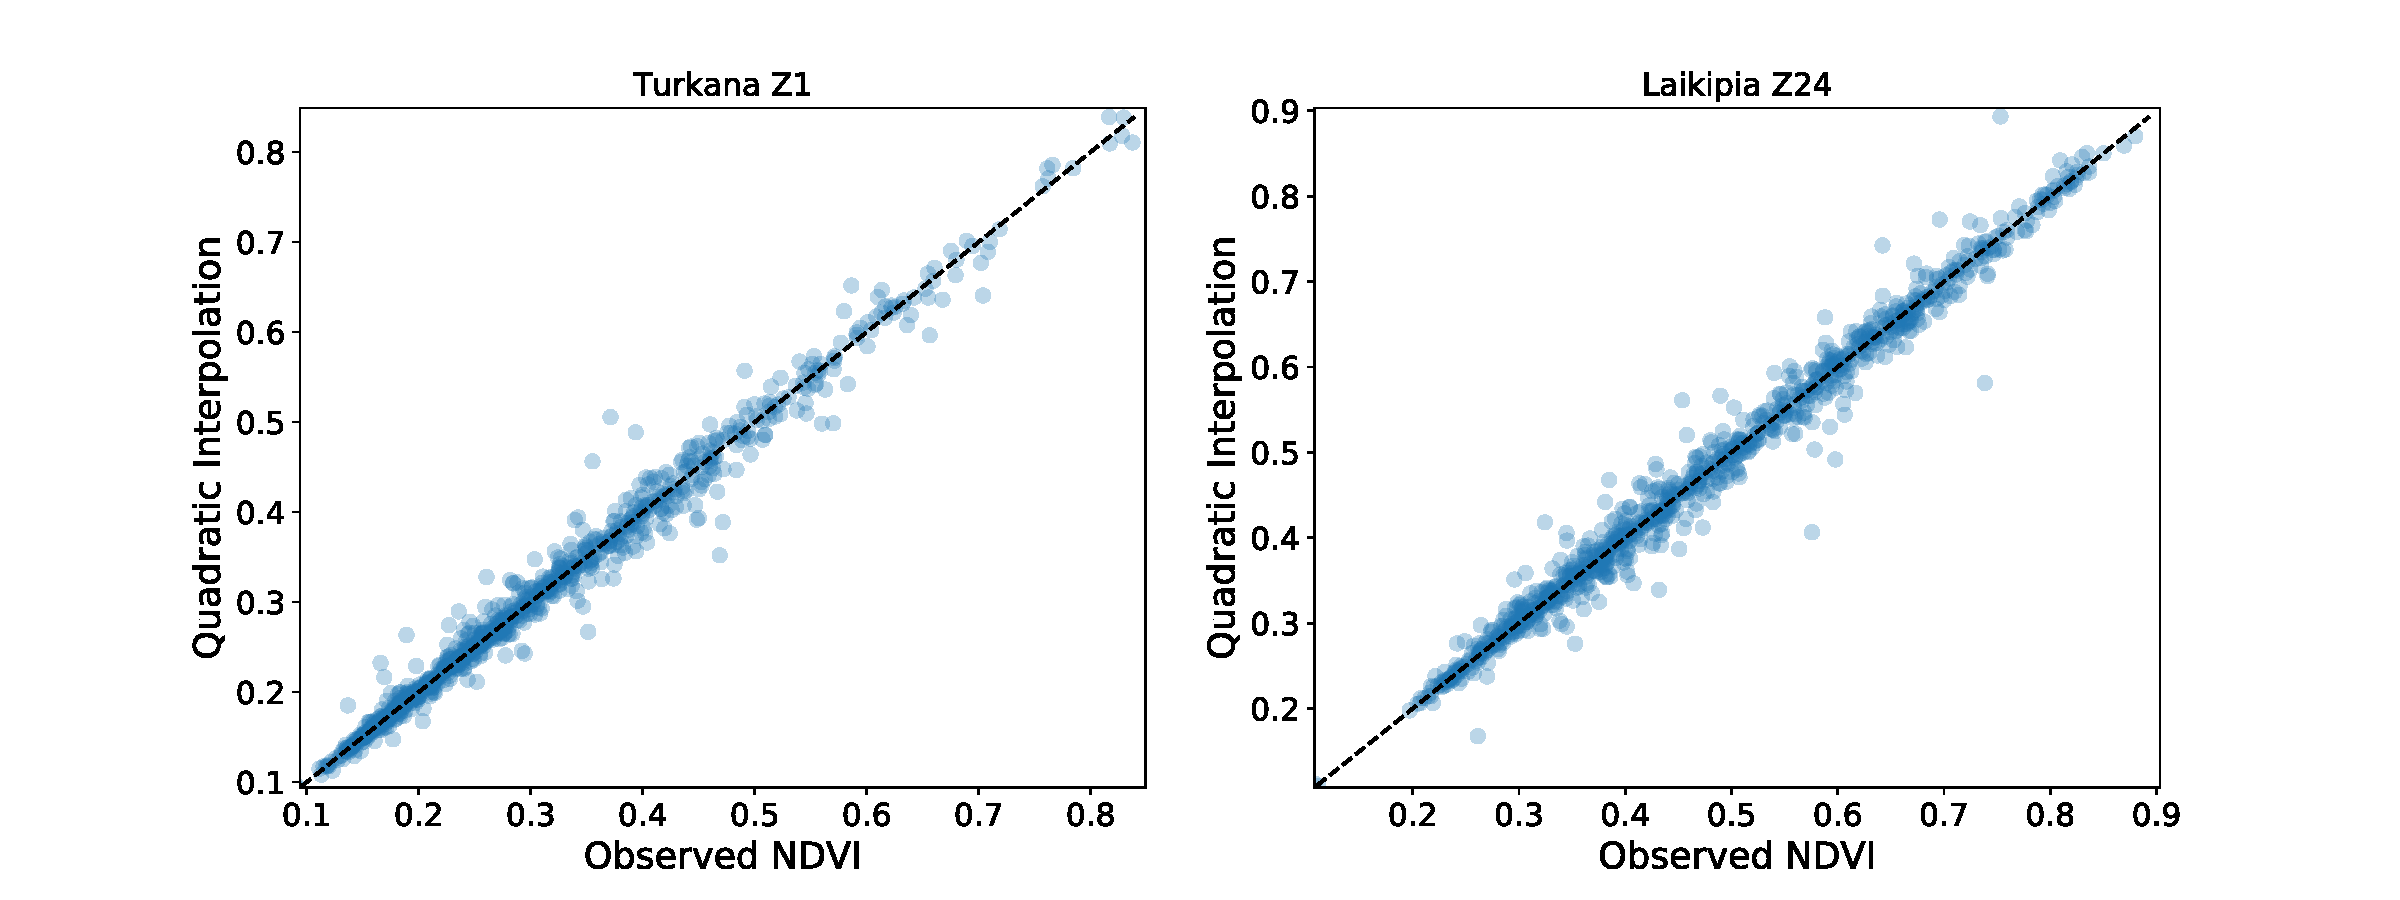
\includegraphics[trim = 15mm 0mm 0mm 0mm,width=15cm]{figures/TurkanaZ1_LaikipiaZ24_Quadratic_Scatter1.pdf} 
	\caption{Scatter plot of MODIS observed and predicted NDVI values for the Quadratic Interpolation gap-filling method for Turkana Zone 1 and Laikipia Zone 24} \label{fig:interpScatter}
\end{figure}

% \begin{figure} 
% 	\centering
% 	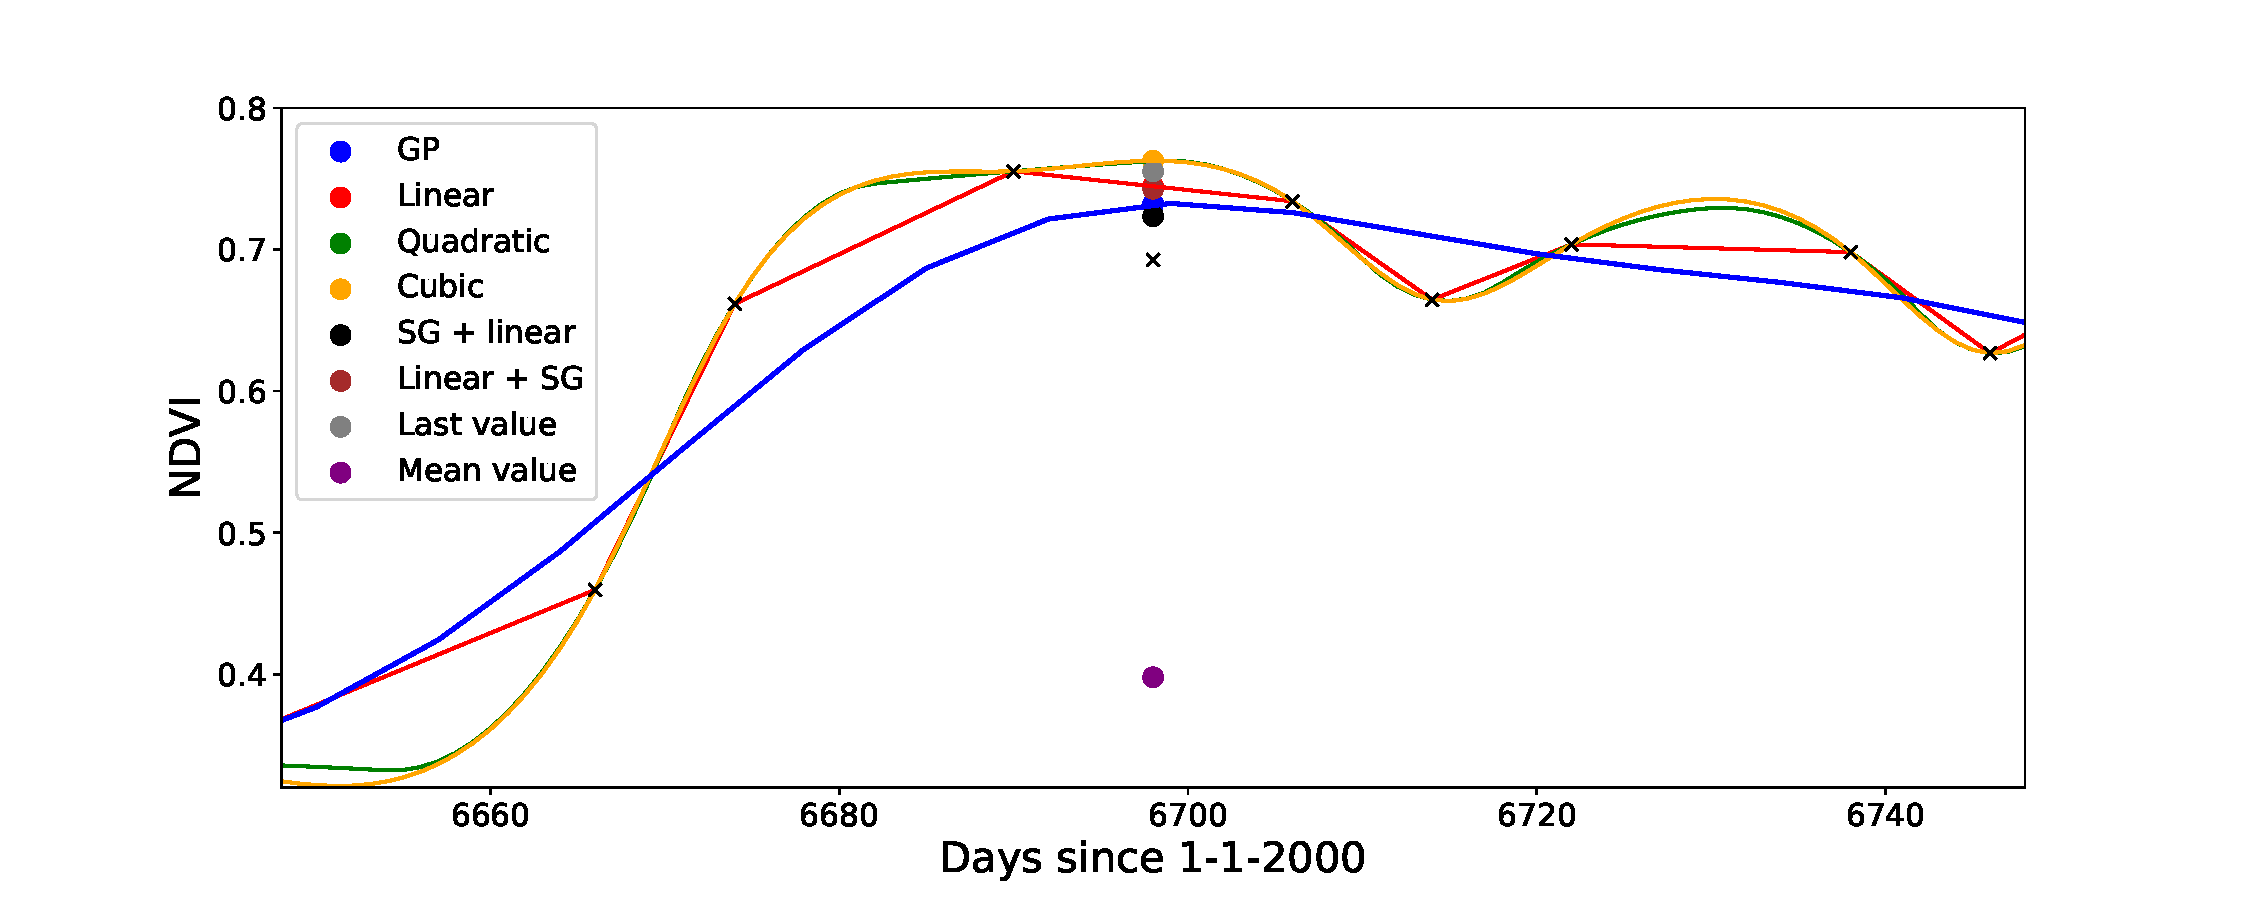
\includegraphics[trim = 35mm 0mm 0mm 0mm,width=12 cm]{figures/interp.pdf} 
% 	\caption{An example of our interpolation method on a Landsat pixel, the black crosses show the real data, where the datum at day 6698 is removed. The colored dots show our interpolated value at day 6698 using the different methods. The blue, red, green and yellow lines show the complete interpolation for every date. } \label{fig:interp}
% \end{figure}


% \begin{figure}
% 	\centering
% 	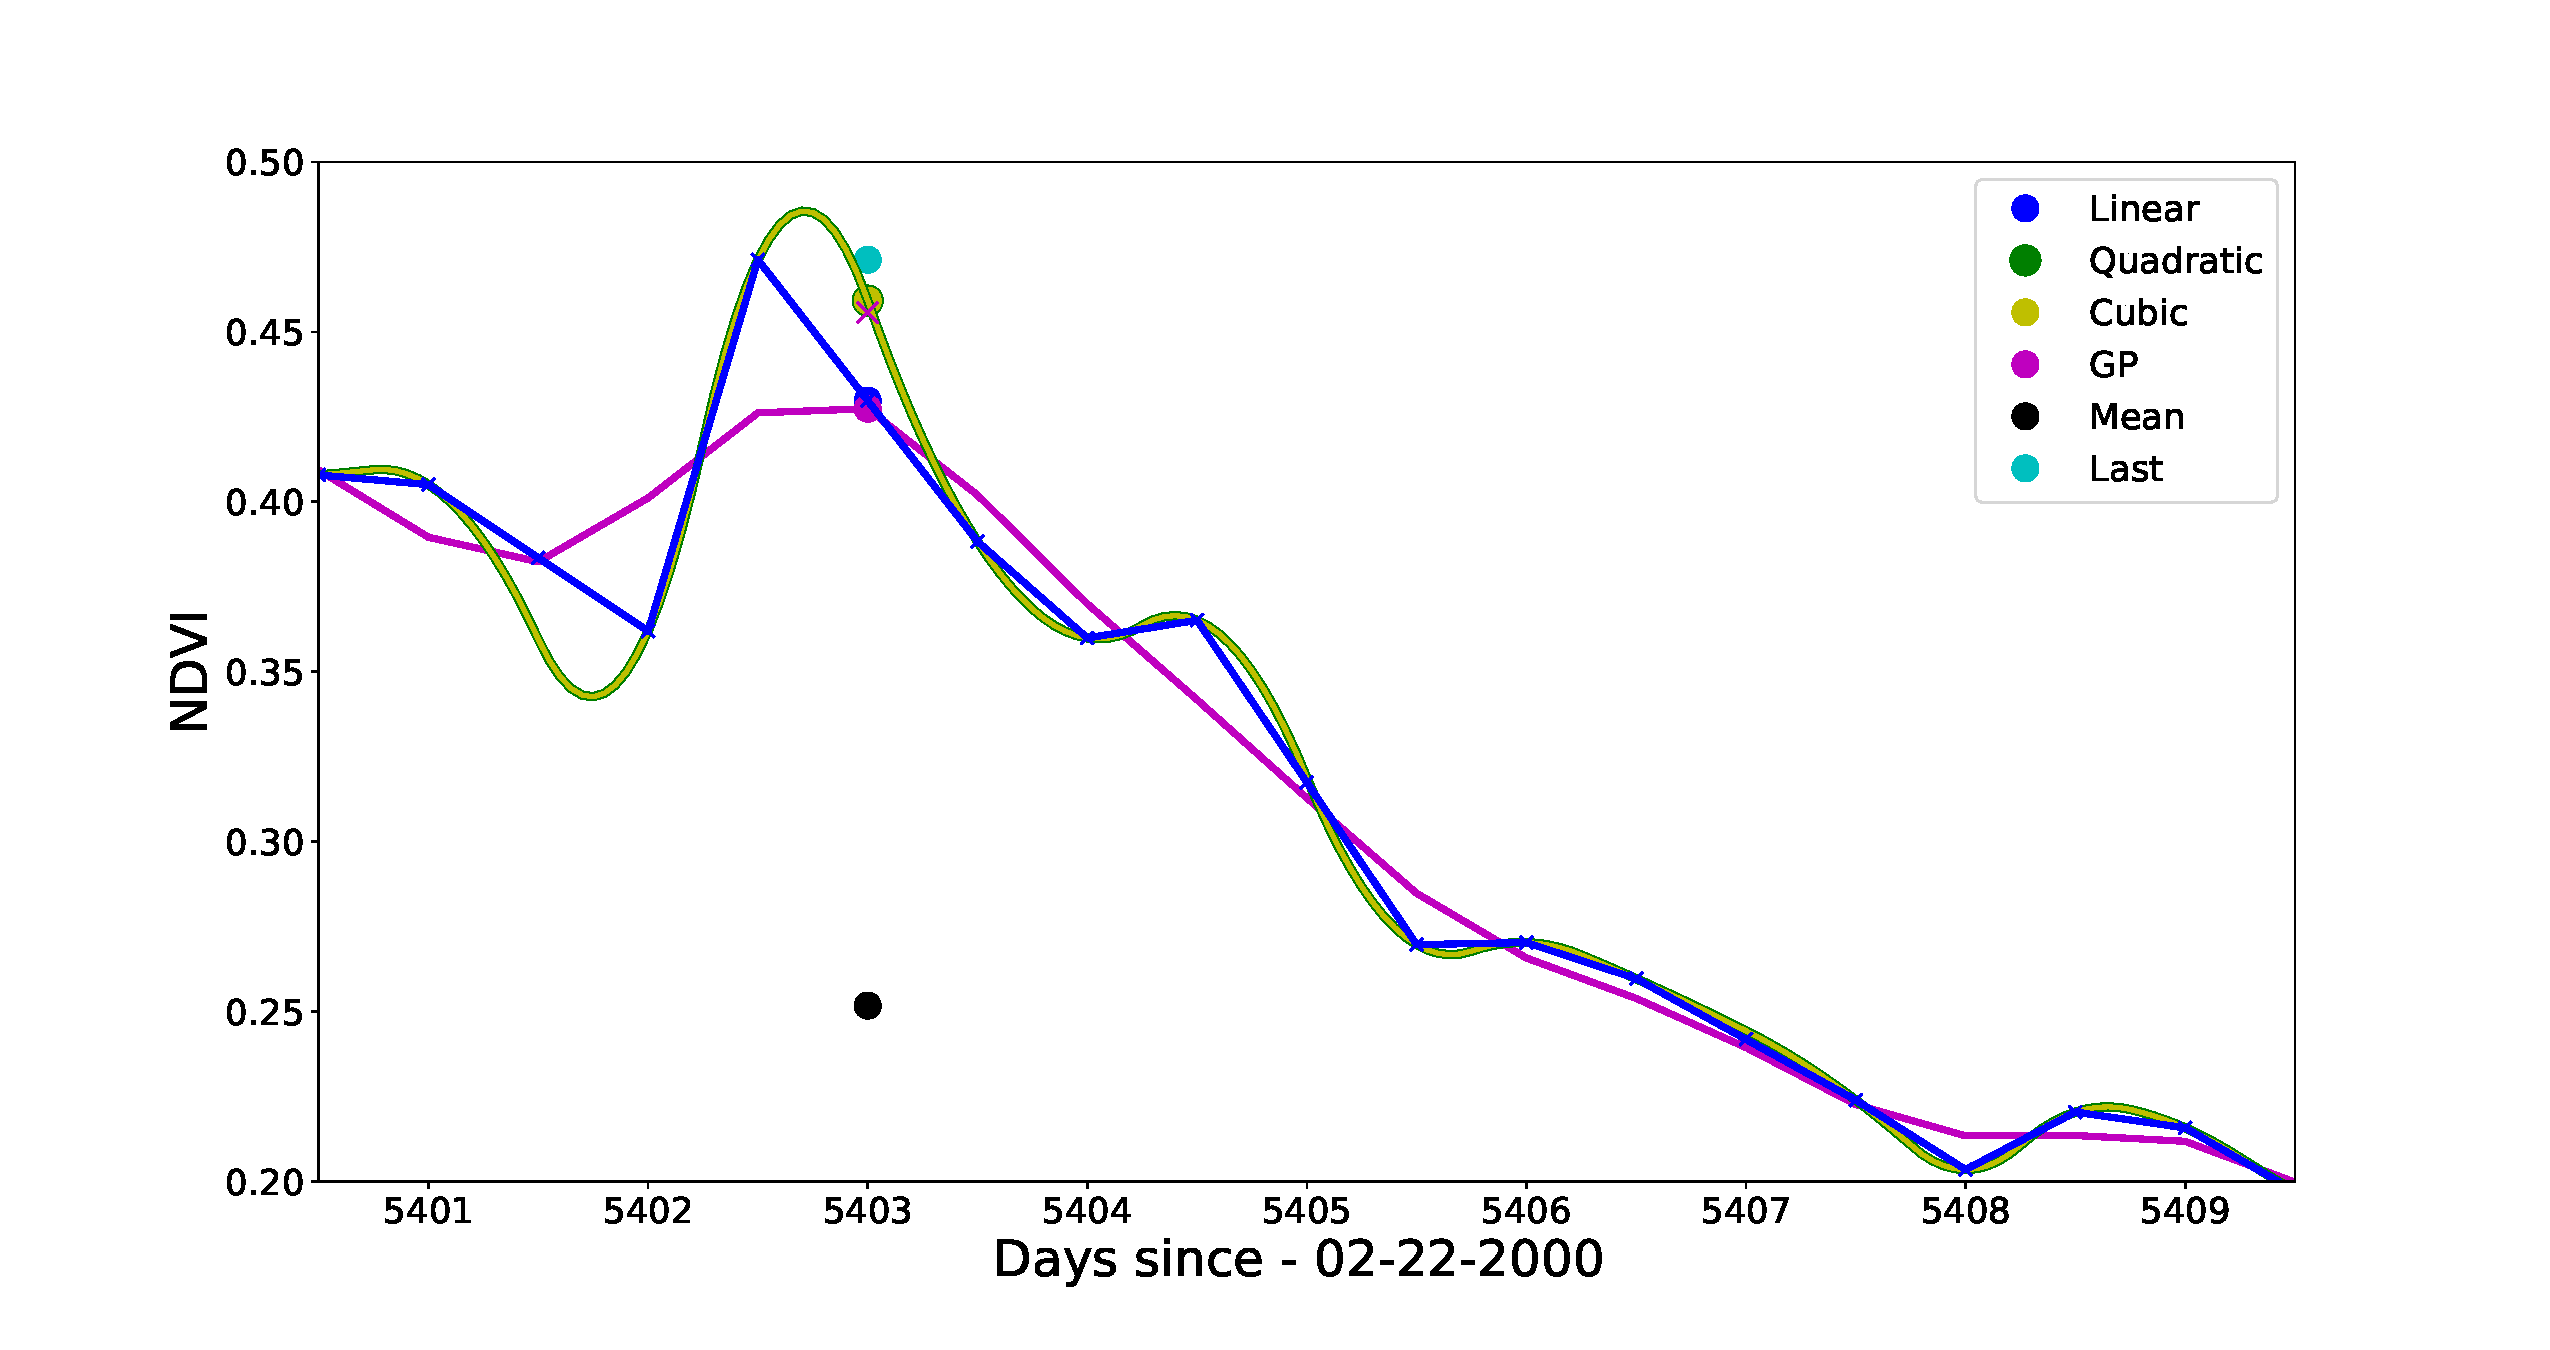
\includegraphics[trim = 35mm 0mm 0mm 0mm,width=12 cm]{figures/interp_2.pdf} 
% 	\caption{An example of interpolation methods on MODIS pixels. The blue cross shows the observation at day 5403, which was then cut and interpolated using different methods. The colored dots show interpolated values using the different methods.  } \label{fig:interp2}
% \end{figure}



\newpage

\section{Forecast}

\begin{figure}
	\centering
	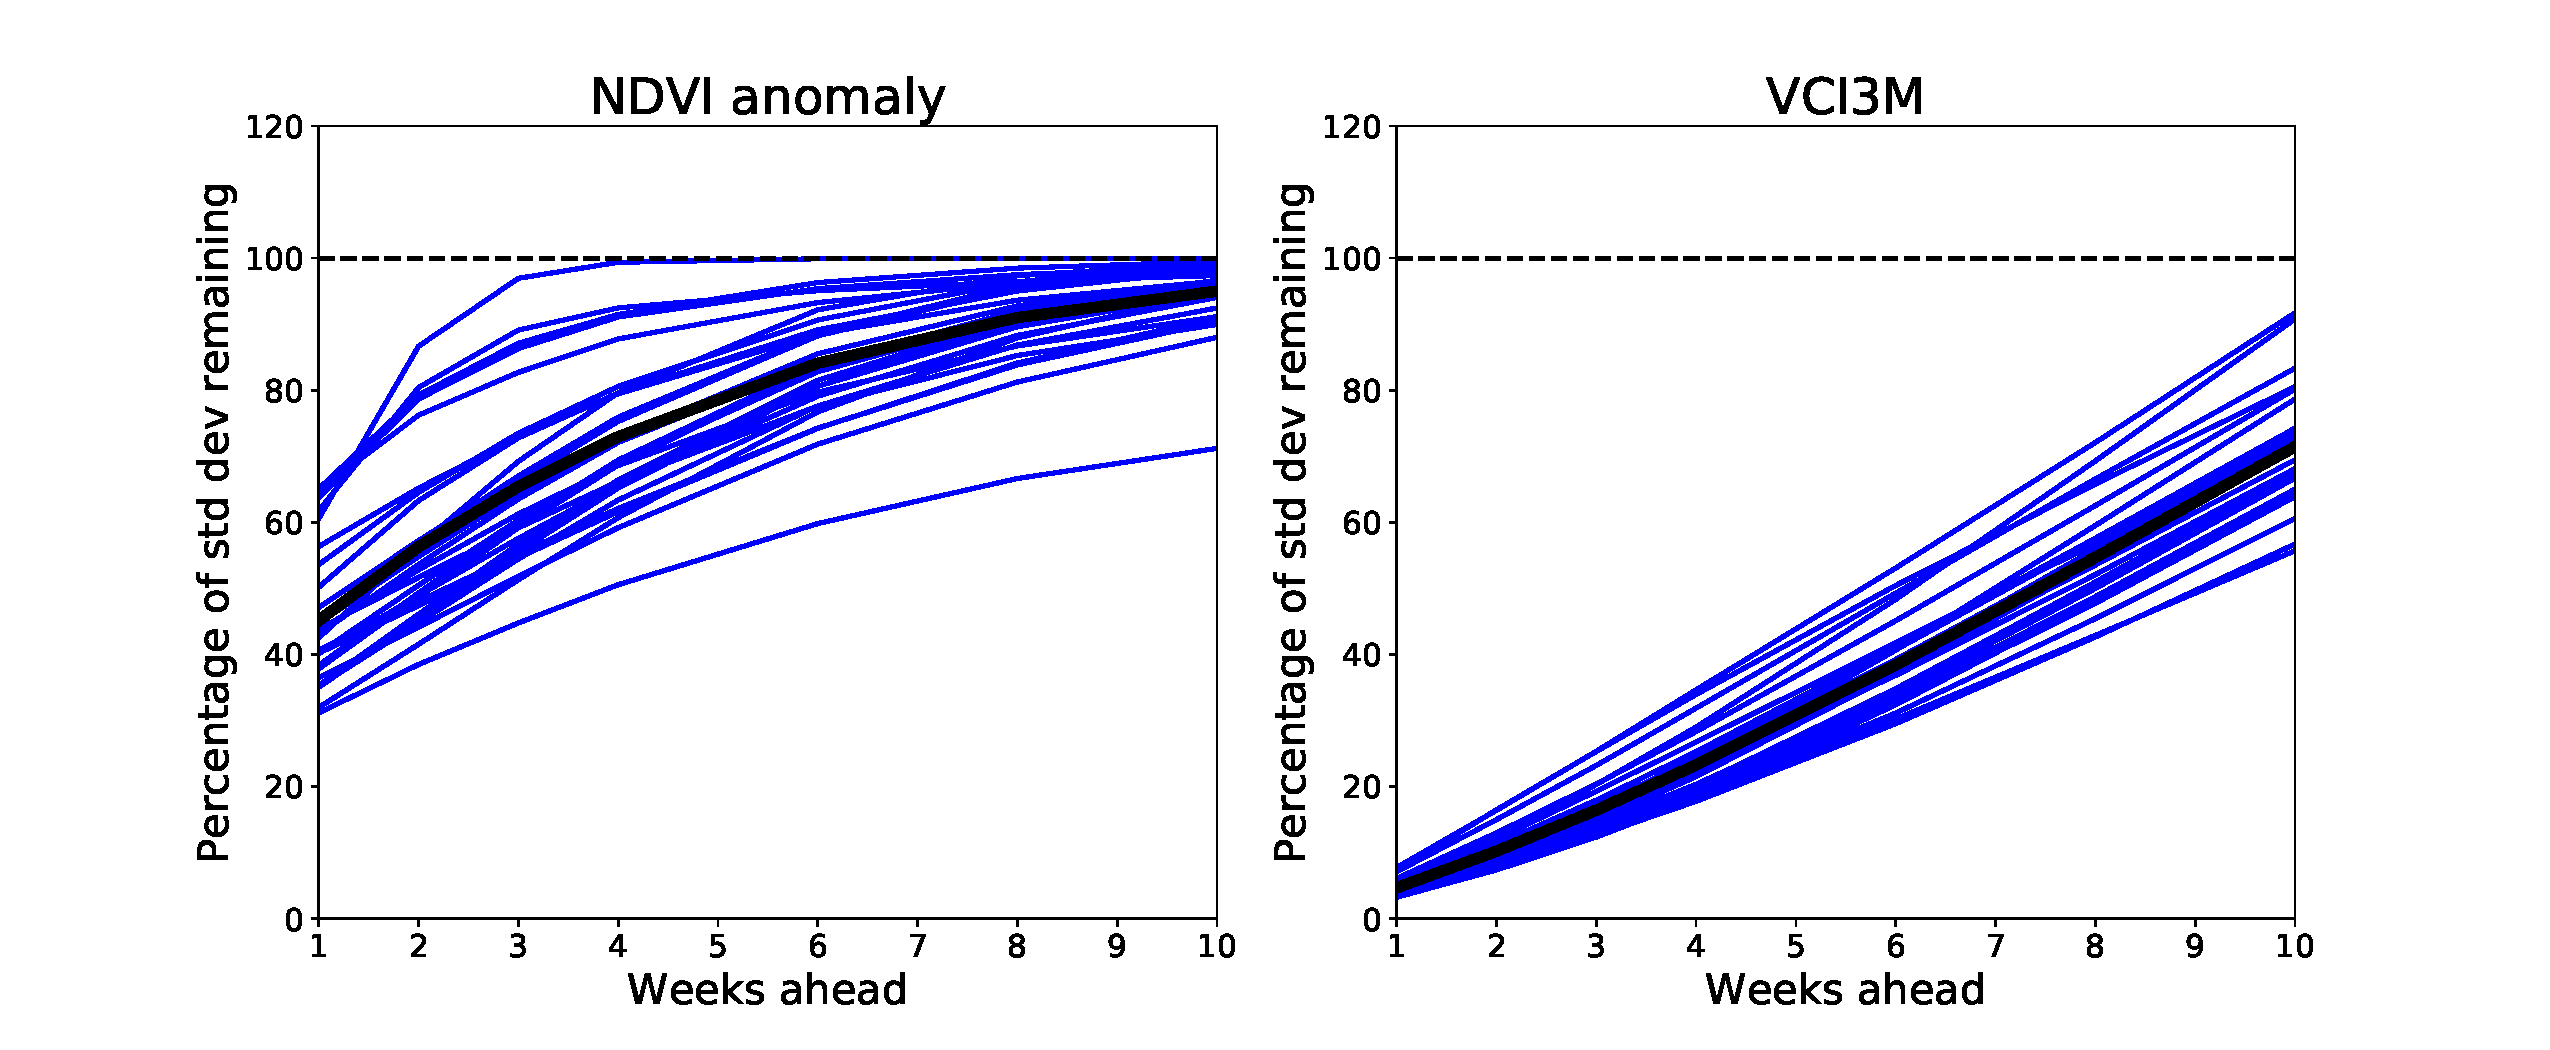
\includegraphics[trim = 50mm 0mm 0mm 0mm,width=14 cm]{figures/FC-pref.pdf} 
	\caption{Forecast performance with a lead time of 1 to 10 weeks using the GP method on the Landsat data, as given by percentage standard deviation remaining $S$, for (Left) NDVI anomaly, and (Right) VCI3M. The blue lines show results for the individual regions (county/livelihood zone intersections), and the black line shows the median across all regions.} \label{fig:GP_NDVI_forecast}
\end{figure}

\begin{figure}
	\centering
	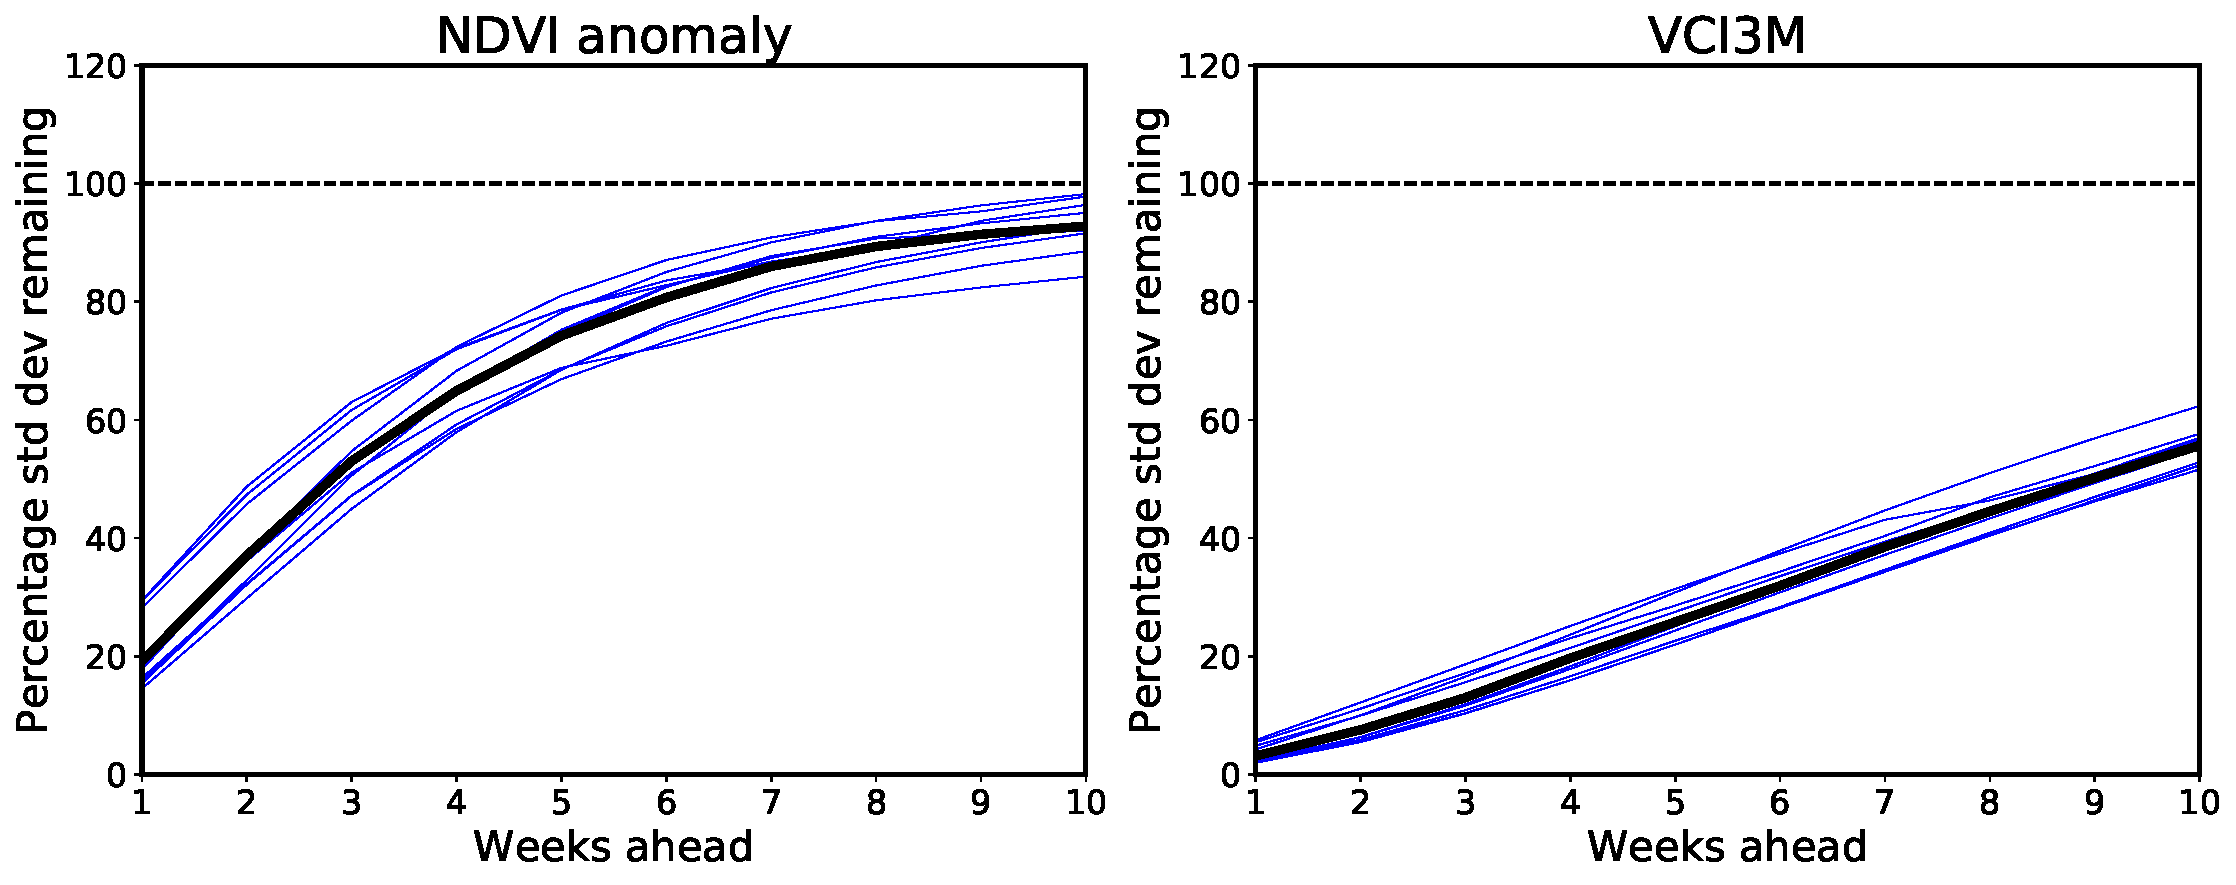
\includegraphics[trim = 20mm 0mm 0mm 0mm,width=12.5cm]{figures/NDVI_forecast2.pdf} 
	\caption{Forecast performance with a lead time of 1 to 10 weeks using the AR method on the MODIS data, as given by percentage standard deviation remaining, for (Left) NDVI anomaly, and (Right) VCI3M. The blue lines show results for the individual regions for which a forecast is possible more than 50\% of the time, and the black line shows the median across all 19 of these regions.} \label{fig:NDVI_forecast}
\end{figure}

\begin{figure}
	\centering
	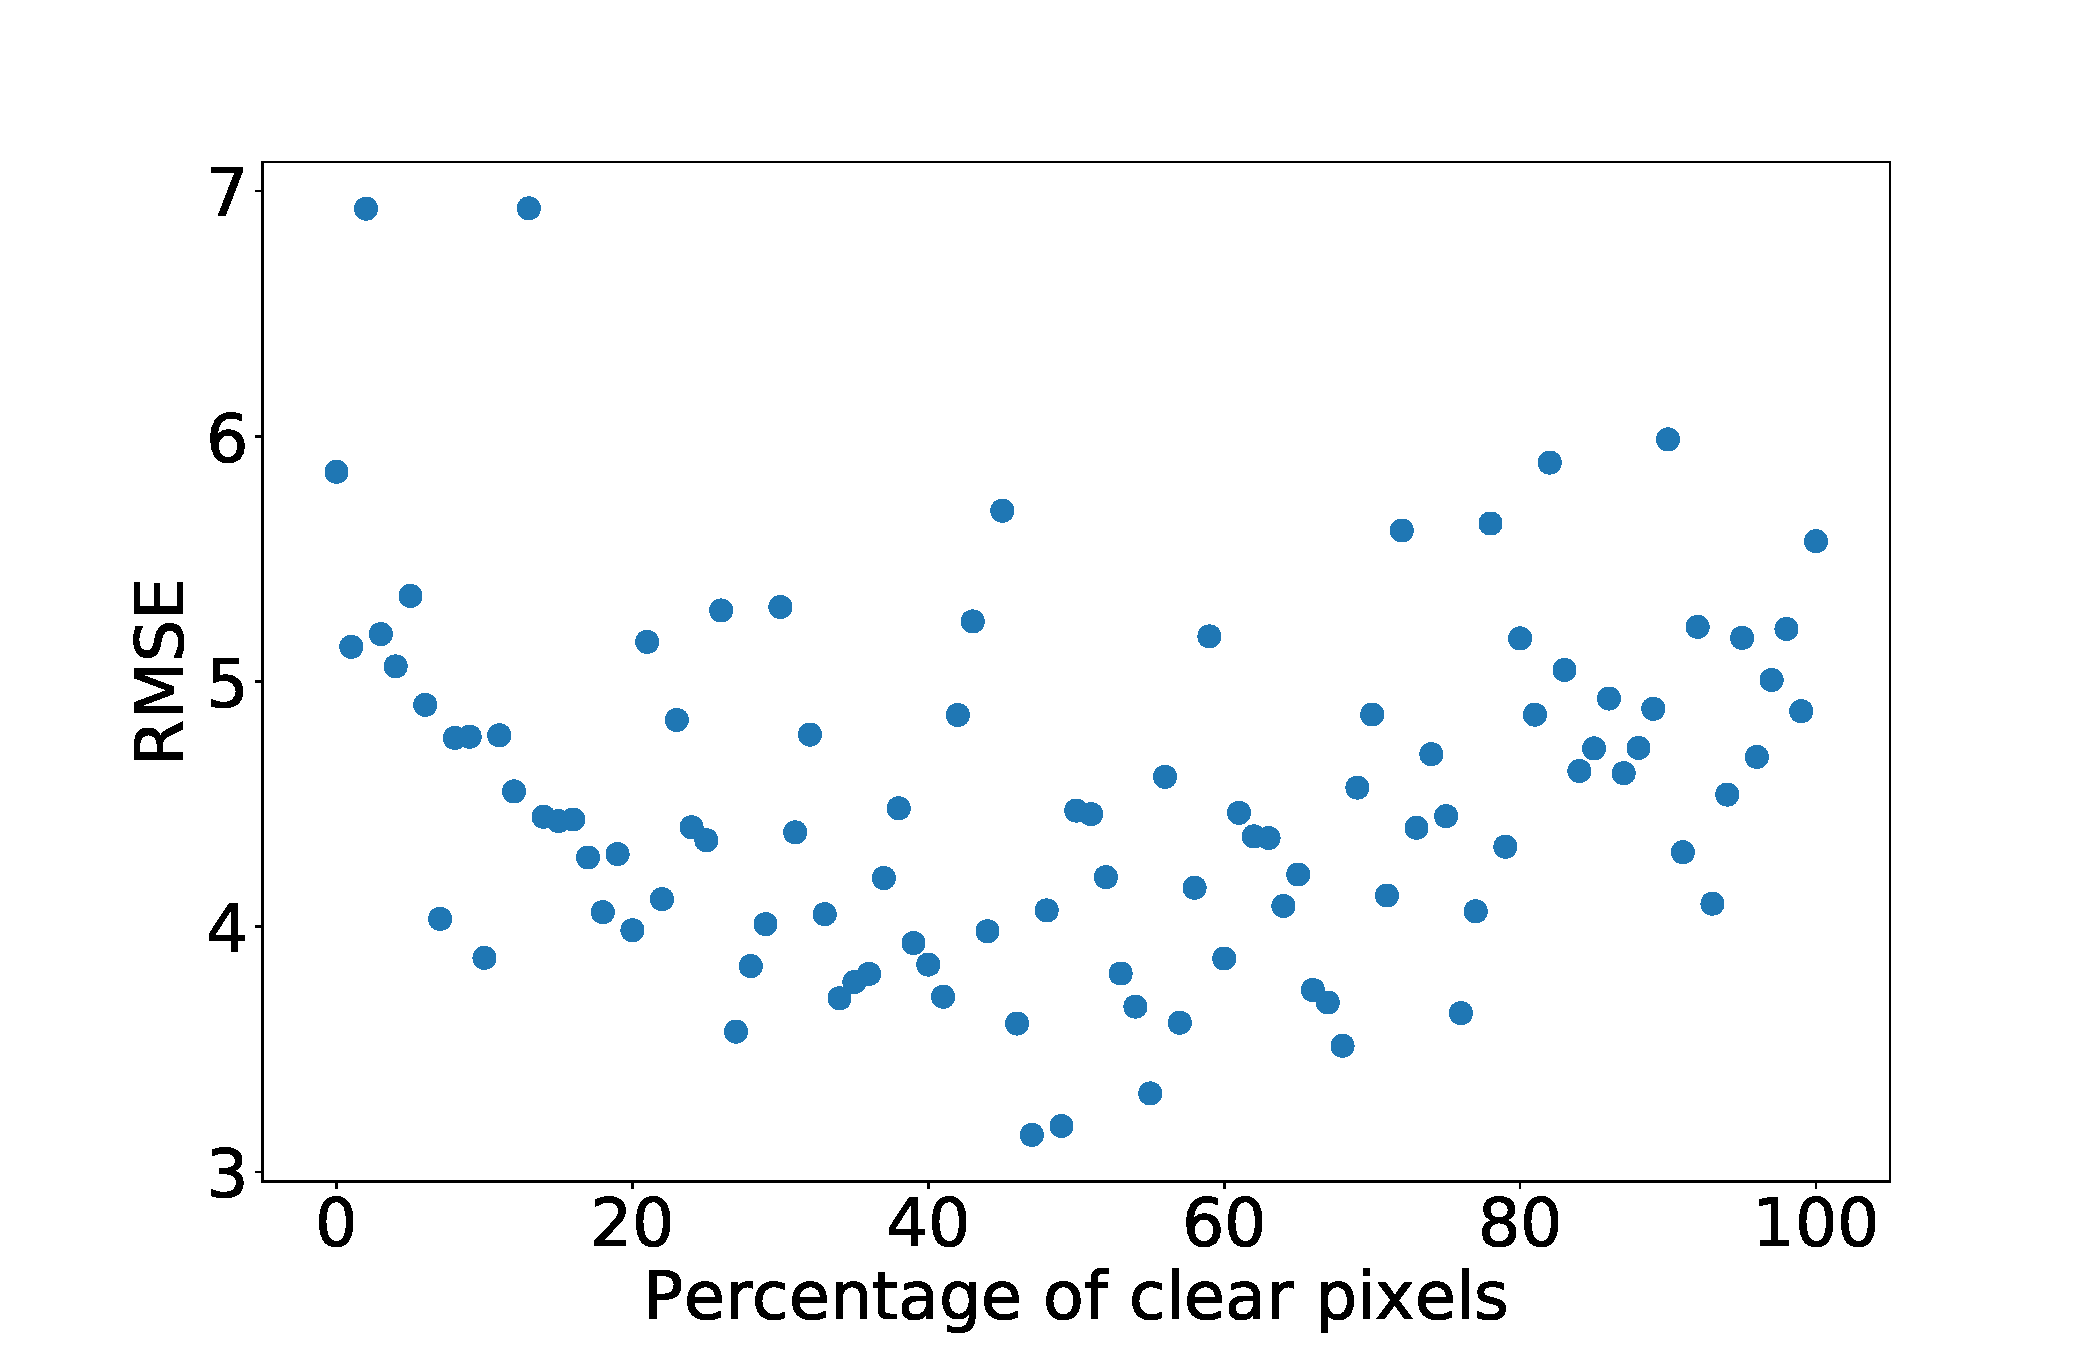
\includegraphics[trim = 30mm 35mm 0mm 10mm,width=5.4 cm]{figures/ngaps.pdf} \qquad 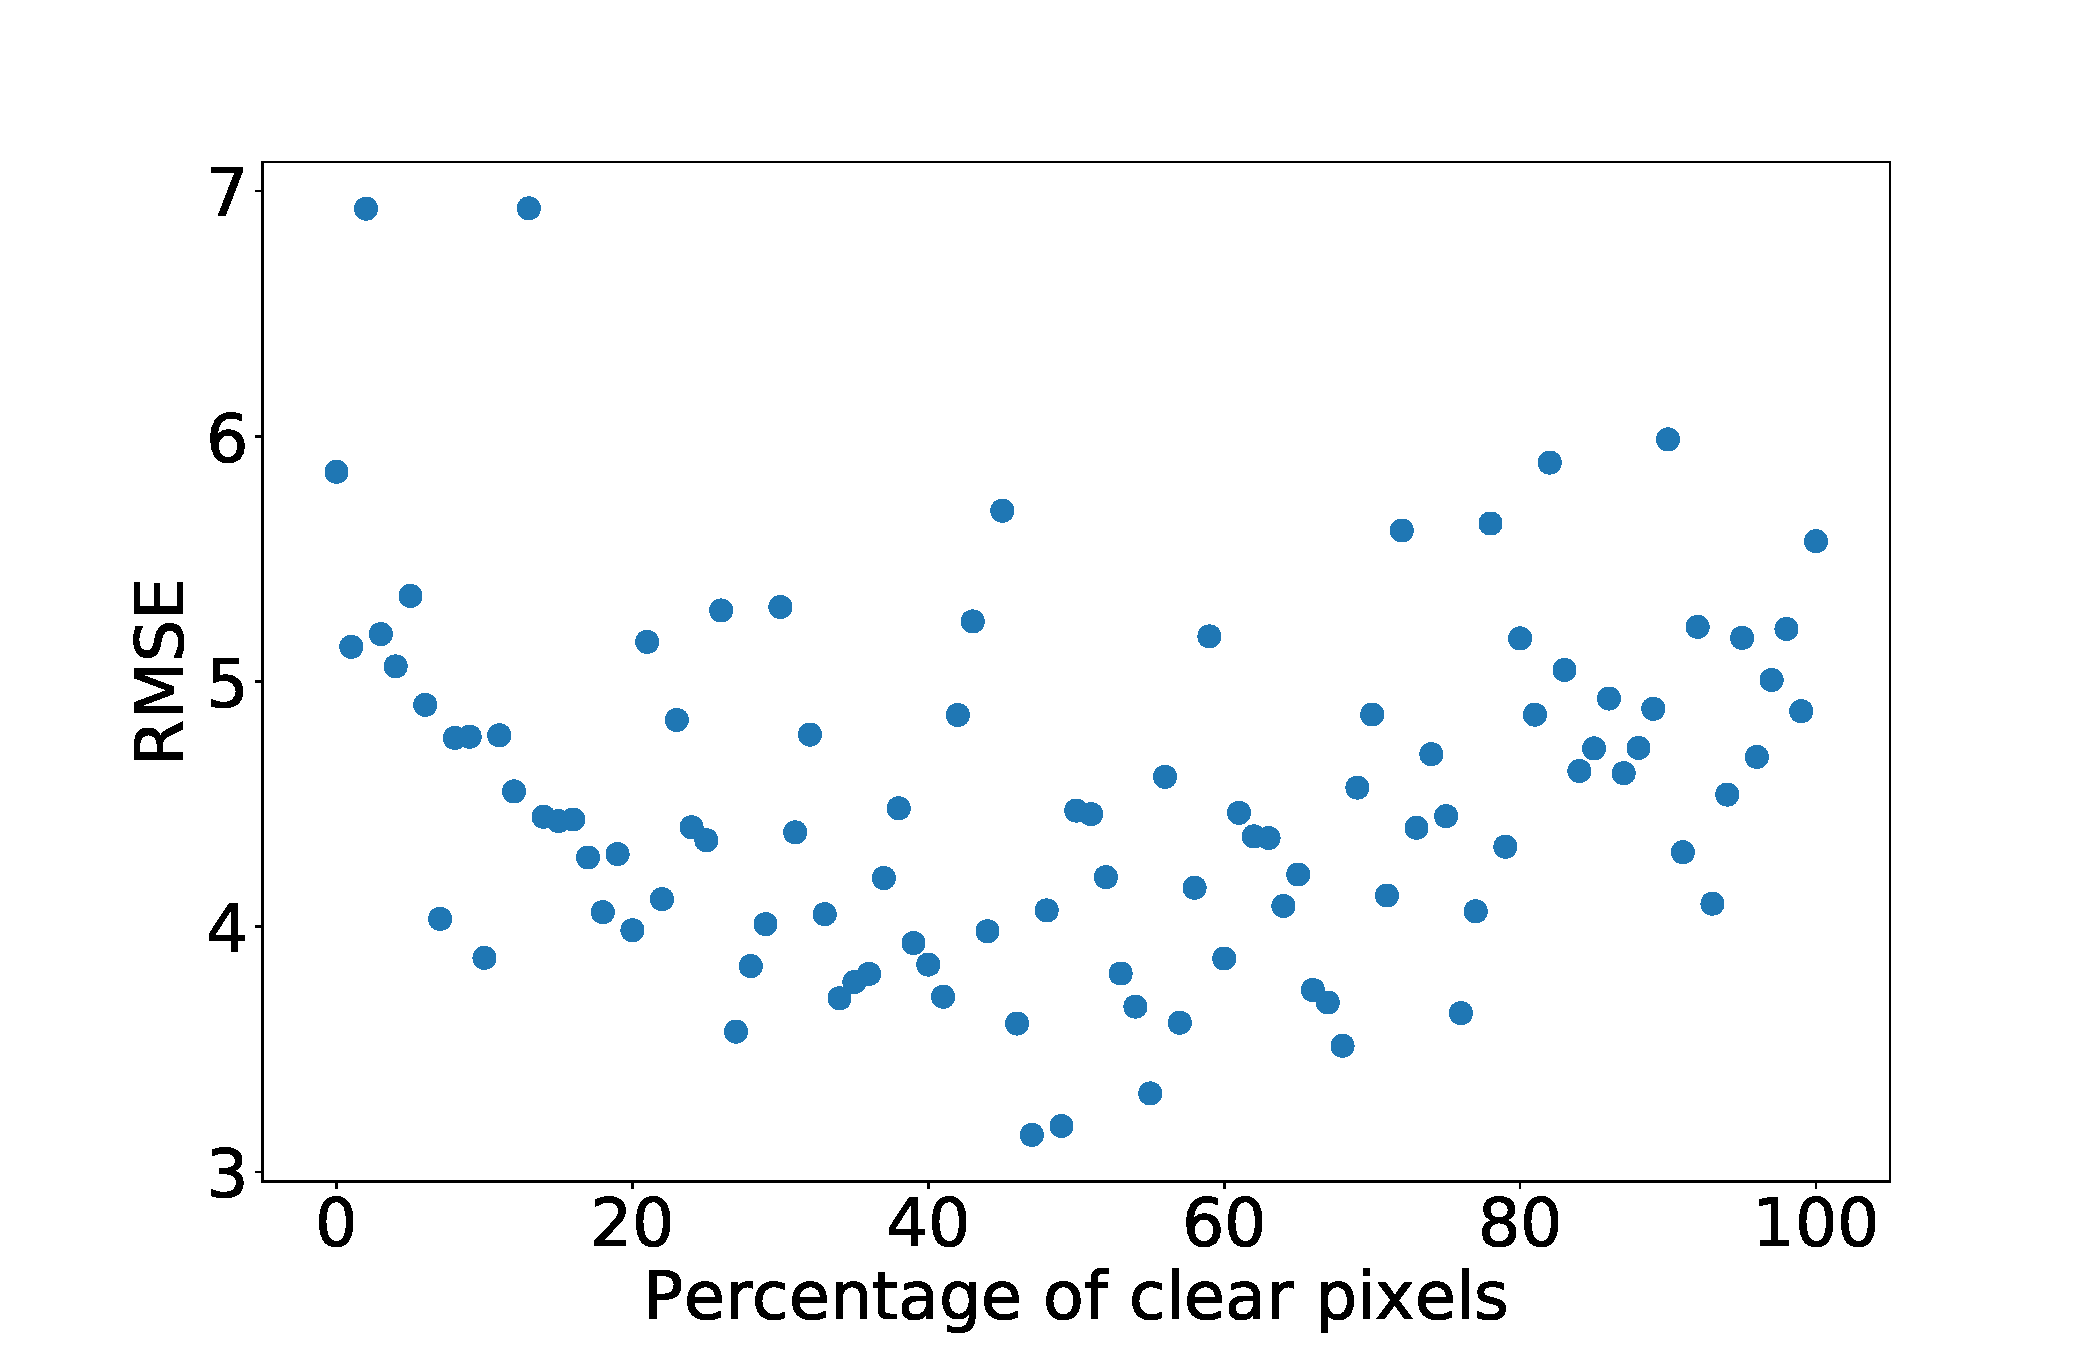
\includegraphics[trim = 0mm 35mm 30mm 10mm,width=5.4 cm]{figures/ngaps.pdf}
	\vspace{0.3cm}
	\caption{\edit{TO DO: STEVEN/EDWARD REPLACE LEFT HAND PLOTS WITH THE CORRESPONDING PLOTS FROM LANDSAT/GP. ADAM: REFERENCE TO THIS FROM MAIN TEXT. RMSE of 4 week forecast against percentage of clear pixels at most recent observation. (Left) Landsat/GP (Right) MODIS/AR, for which the Pearson correlation is 0.01.}} \label{fig:ROCotherdrought}
\end{figure}

\begin{figure}
	\centering
	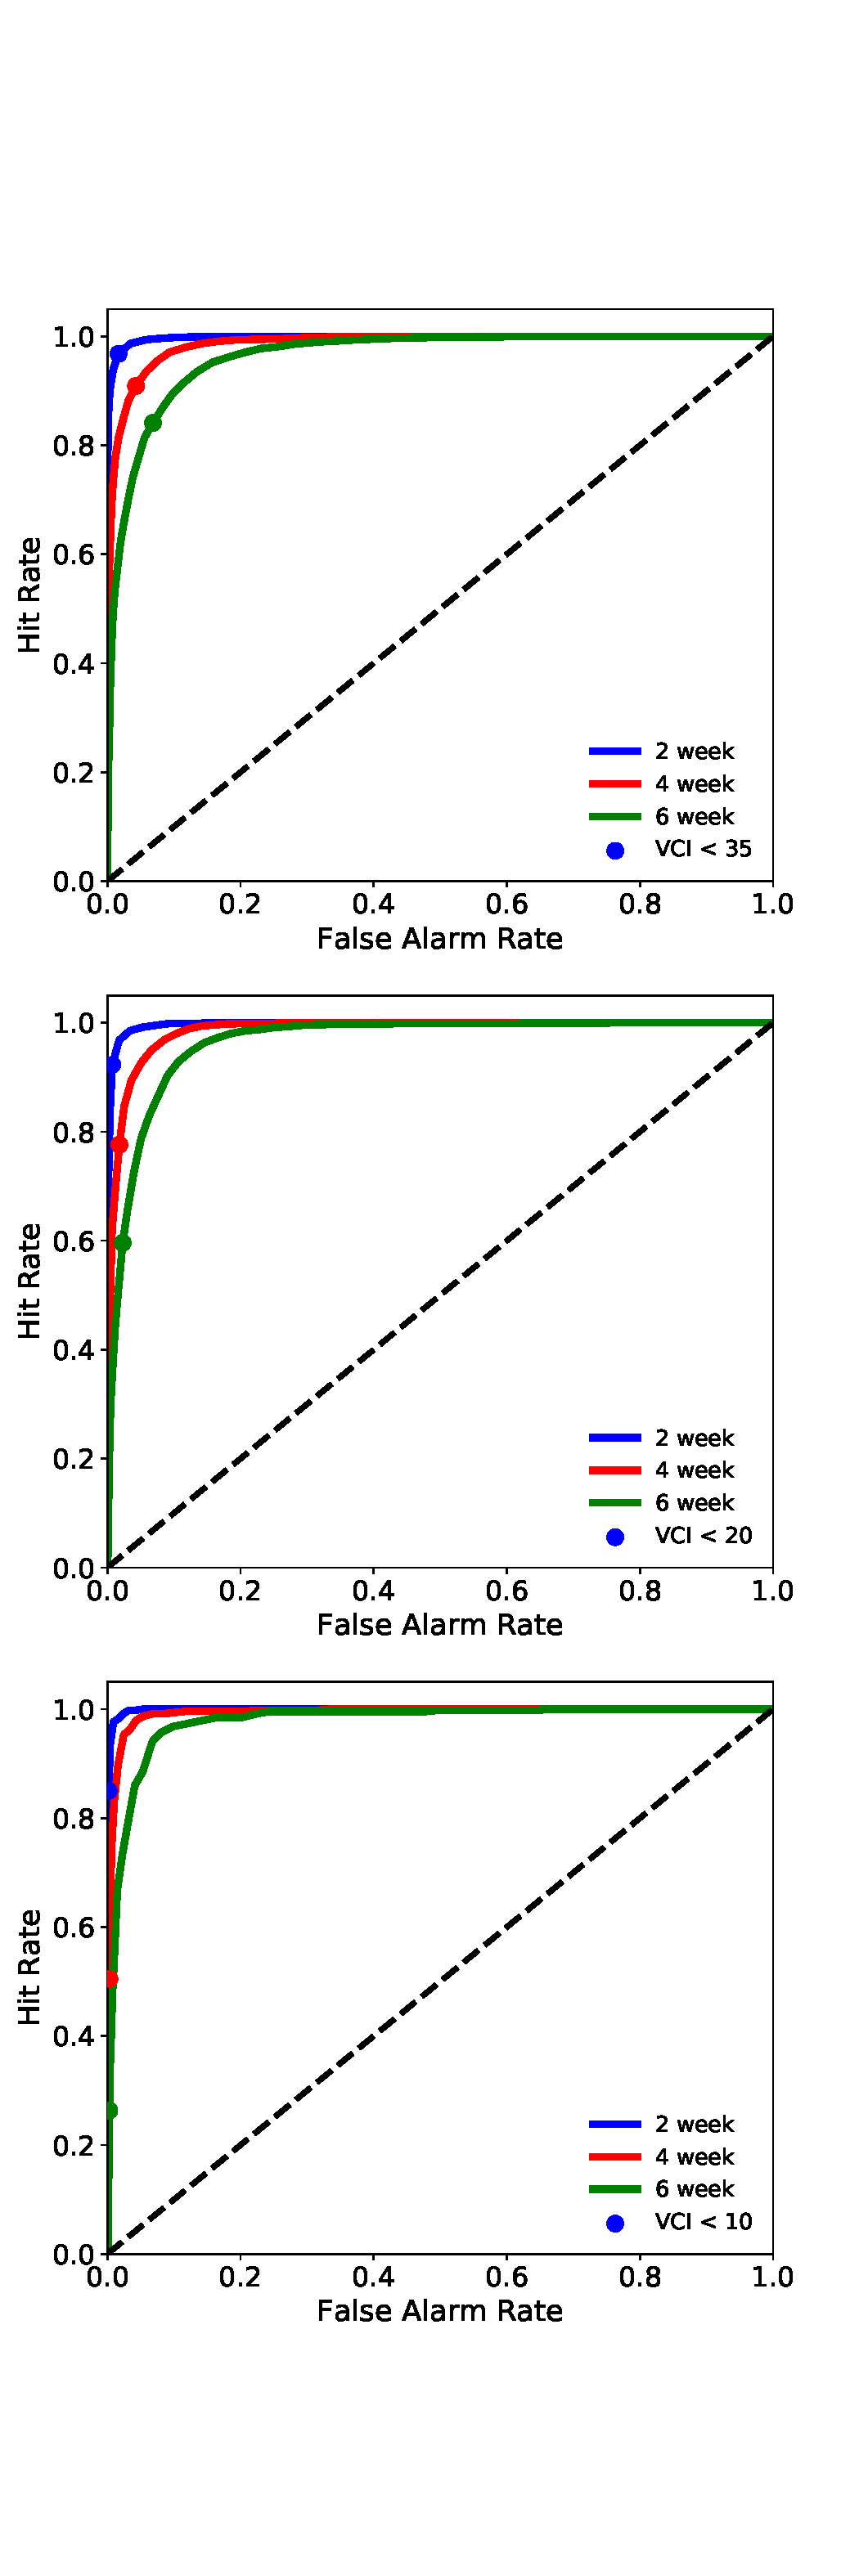
\includegraphics[trim = 30mm 35mm 0mm 10mm,width=5.4 cm]{figures/VCIotherROCabb.pdf} \qquad 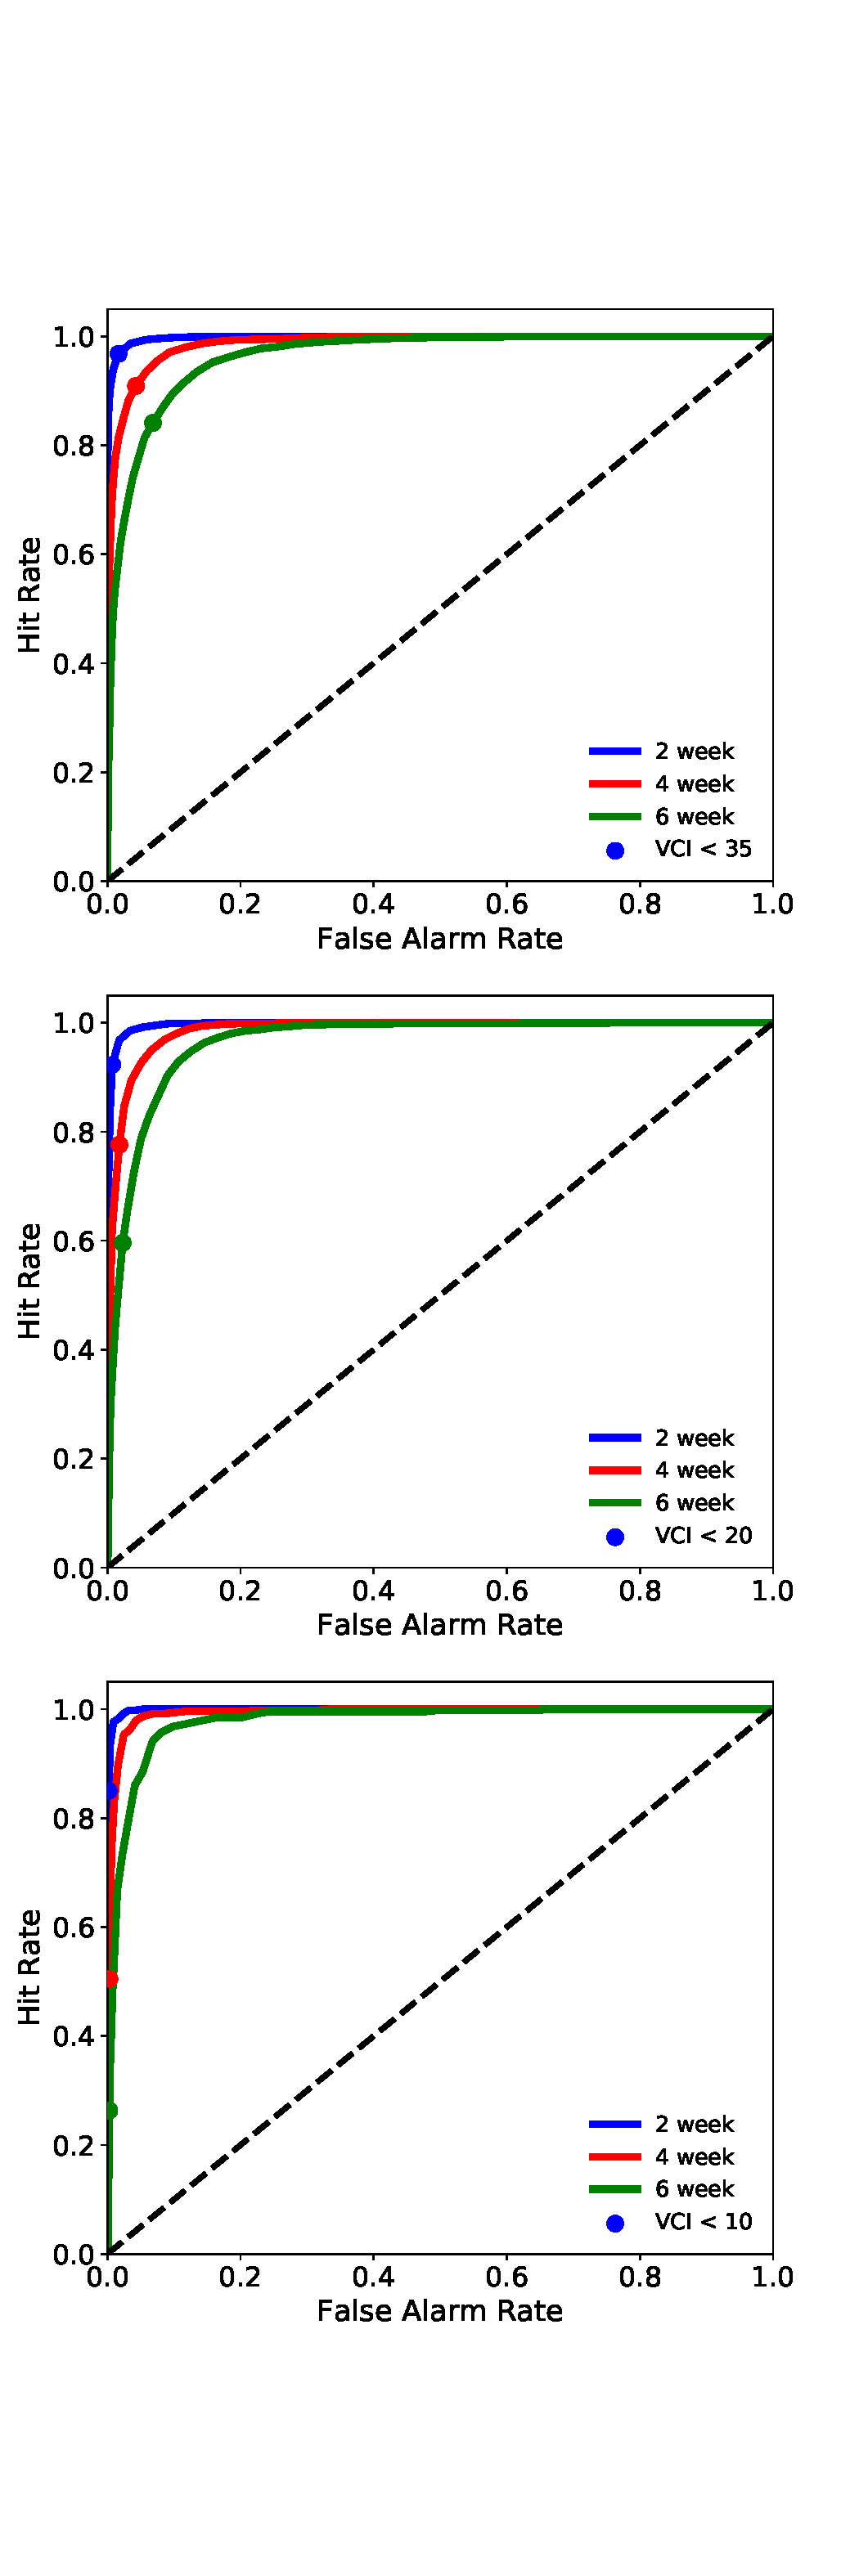
\includegraphics[trim = 0mm 35mm 30mm 10mm,width=5.4 cm]{figures/VCIotherROCabb.pdf}
	\caption{\edit{TO DO: ADAM REPLACE LEFT HAND PLOTS WITH THE CORRESPONDING PLOTS FROM LANDSAT/GP. ROC curves for predicting drought with drought defined at various NDMA thresholds. For (Left) Landsat/GP (Right) MODIS/AR: (Top) Any drought,} VCI3M$<$35, \edit{(Middle) Severe or extreme drought} VCI3M$<$20,\edit{ (Bottom) Extreme drought} VCI3M$<$10.} \label{fig:ROCotherdrought}
\end{figure}



\newpage
\subsection{Tables of NDVI and VCI3M forecast} \label{app}

\begin{table}
	\footnotesize
	\caption{NDVI anomaly forecast using Landsat data for the 29 regions. The numbers shown are the proportion of standard deviation remaining (Equation \ref{eq:S}) and the $R^2$-score for NDVI anomaly. We only used past data for the interpolation and we the average value for every pixel within the region for the region estimate. The * indicates regions where a minimum of 180 detections per pixel where used, instead of 250. } \label{tab:NDVI_LS}
	\centering
	\begin{tabular}{l|ccc} 
		\toprule
		\textbf{Region}   & \textbf{2 weeks}  & \textbf{4 weeks}  & \textbf{6 weeks} \\
		\midrule
		Baringo Z24 & 46 0.74 & 66 0.46 & 81 0.19 \\
		Elgeyo-Marakwet Z24 & 49 0.74 & 69 0.47 & 83 0.22 \\
		Garissa Z10* & 55 0.64 & 73 0.36 & 86 0.12 \\
		Garissa Z11* & 63 0.58 & 80 0.33 & 89 0.16 \\
		Isiolo Z5 & 57 0.64 & 75 0.37 & 88 0.13 \\
		Isiolo Z9 & 65 0.53 & 79 0.30 & 89 0.13 \\
		Isiolo Z10 & 79 0.31 & 91 0.08 & 96 -0.02 \\
		Isiolo Z24 & 57 0.67 & 76 0.41 & 89 0.19 \\
		Kajiado Z15 & 45 0.76 & 63 0.52 & 78 0.28 \\
		Kajiado Z18* & 44 0.75 & 59 0.55 & 72 0.34 \\
		Laikipia Z24 & 42 0.82 & 61 0.62 & 77 0.39 \\
		Lamu Z11* & 80 0.33 & 92 0.12 & 95 0.07 \\
		Mandera Z7 & 76 0.25 & 88 0.00 & 93 -0.13 \\
		Mandera Z9 & 53 0.44 & 69 0.06 & 80 -0.27 \\
		Marsabit Z5 & 52 0.60 & 66 0.35 & 78 0.11 \\
		Marsabit Z7* & 47 0.76 & 62 0.59 & 74 0.40 \\
		Narok Z15 & 56 0.67 & 80 0.34 & 92 0.12 \\
		Narok Z18 & 56 0.68 & 75 0.42 & 88 0.20 \\
		Samburu Z5 & 49 0.68 & 69 0.36 & 84 0.08 \\
		Samburu Z24 & 45 0.78 & 65 0.54 & 81 0.30 \\
		Tana River Z11* & 65 0.57 & 81 0.33 & 91 0.15 \\
		Turkana Z1 & 54 0.56 & 72 0.21 & 84 -0.09 \\
		Turkana Z3 & 38 0.61 & 51 0.33 & 60 0.06 \\
		Turkana Z24 & 46 0.75 & 66 0.48 & 81 0.21 \\
		Wajir Z7* & 48 0.71 & 62 0.51 & 74 0.30 \\
		Wajir Z9 & 79 0.20 & 91 -0.07 & 95 -0.18 \\
		Wajir Z10 & 87 0.24 & 99 0.01 & 100 0.00 \\
		WestPokot Z1 & 50 0.69 & 69 0.43 & 83 0.18 \\
		WestPokot Z24 & 49 0.68 & 66 0.42 & 79 0.16 \\
		\bottomrule
		Median & 53 0.67 & 69 0.36 & 84 0.15 \\
		\bottomrule
	\end{tabular}
\end{table}



\begin{table}
	\footnotesize
	\caption{VCI3M forecast performance using GPs on the Landsat data. The numbers shown are the percentage standard deviation remaining and the $R^2$ score, respectively.} \label{tab:VCI_LS}
	\centering
	%% \tablesize{} %% You can specify the fontsize here, e.g.,  \tablesize{\footnotesize}. If commented out \small will be used.
	\begin{tabular}{l|ccc} 
		\toprule
		\textbf{Region}  &  \textbf{2 weeks} &  \textbf{4 weeks}  & \textbf{6 weeks}  \\
		\midrule
		Baringo Z24 & 9 0.99 & 22 0.95 & 38 0.86 \\
		Elgeyo-Marakwet Z24 & 9 0.99 & 21 0.96 & 36 0.87 \\
		Garissa Z10 & 10 0.99 & 23 0.95 & 39 0.85 \\
		Garissa Z11 & 11 0.99 & 25 0.94 & 41 0.83 \\
		Isiolo Z5 & 10 0.99 & 23 0.95 & 39 0.85 \\
		Isiolo Z9 & 11 0.99 & 24 0.94 & 38 0.85 \\
		Isiolo Z10 & 13 0.98 & 29 0.92 & 46 0.79 \\
		Isiolo Z24 & 10 0.99 & 23 0.95 & 39 0.85 \\
		Kajiado Z15 & 9 0.99 & 21 0.96 & 36 0.87 \\
		Kajiado Z18 & 9 0.99 & 20 0.96 & 34 0.88 \\
		Laikipia Z24 & 7 0.99 & 18 0.97 & 32 0.89 \\
		Lamu Z11 & 13 0.98 & 29 0.92 & 45 0.80 \\
		Mandera Z7 & 15 0.98 & 32 0.90 & 49 0.76 \\
		Mandera Z9 & 12 0.98 & 29 0.92 & 48 0.77 \\
		Marsabit Z5 & 11 0.99 & 25 0.94 & 41 0.83 \\
		Marsabit Z7 & 8 0.99 & 19 0.96 & 32 0.90 \\
		Narok Z15 & 10 0.99 & 25 0.94 & 41 0.83 \\
		Narok Z18 & 11 0.99 & 24 0.94 & 40 0.84 \\
		Samburu Z5 & 10 0.99 & 24 0.94 & 42 0.83 \\
		Samburu Z24 & 8 0.99 & 20 0.96 & 35 0.88 \\
		TanaRiver Z11 & 11 0.99 & 24 0.94 & 40 0.84 \\
		Turkana Z1 & 14 0.98 & 31 0.90 & 52 0.73 \\
		Turkana Z3 & 12 0.99 & 26 0.93 & 43 0.81 \\
		Turkana Z24 & 9 0.99 & 22 0.95 & 38 0.85 \\
		Wajir Z7 & 9 0.99 & 20 0.96 & 34 0.88 \\
		Wajir Z9 & 16 0.97 & 35 0.88 & 53 0.72 \\
		Wajir Z10 & 17 0.97 & 35 0.88 & 52 0.73 \\
		WestPokot Z1 & 9 0.99 & 23 0.95 & 39 0.85 \\
		WestPokot Z24 & 10 0.99 & 22 0.95 & 38 0.85 \\
		\bottomrule
		Median & 10 0.99 & 24 0.94 & 39 0.85 \\
		\bottomrule
	\end{tabular}
\end{table}



\begin{table}
	\footnotesize
	\caption{VCI3M forecast performance using AR on the MODIS data. The numbers shown are the percentage standard deviation remaining and the $R^2$ score, respectively. In the 'Forecasts' column, the number gives the percentage of time points for which it was possible to obtain a forecast.  } \label{tab:VCI3m_MODIS}
	\centering
	%% \tablesize{} %% You can specify the fontsize here, e.g.,  \tablesize{\footnotesize}. If commented out \small will be used.
	\begin{tabular}{l|ccc|c} 
		\toprule
		\textbf{Region}  &  \textbf{2 weeks} &  \textbf{4 weeks}  & \textbf{6 weeks} & \textbf{Forecasts} \\
		\midrule
		Baringo Z24 & 	6 	0.99 	& 	18 	0.96 	& 	32 	0.89 & 100\\
		Elgeyo-Marakwet Z24 &  6 	0.99 	& 	18 	0.96 	& 	32 	0.89 & 95 	\\
		Garissa Z10 &  11 	0.98 	& 	20 	0.95 	& 	53 	0.71 & 15	\\
		Garissa Z11 & xx xx & xx xx & xx xx & 0 \\
		Isiolo Z5 & 12 	0.98 	& 	27 	0.92 	& 	42 	0.81 & 97	 \\
		Isiolo Z9 &  13 	0.98 	& 	28 	0.91 	& 	43 	0.81 & 89	\\
		Isiolo Z10 & 13 	0.98 	& 	28 	0.91 	& 	42 	0.81 & 71\\
		Isiolo Z24 & 8 	0.99 	& 	22 	0.95 	& 	37 	0.86 & 93	\\
		Kajiado Z15 & 12 	0.98 	& 	26 	0.92 	& 	39 	0.84 & 75\\
		Kajiado Z18& 11 	0.98 	& 	24 	0.94 	& 	38 	0.85 & 71\\
		Laikipia Z24 & 9 	0.99 	& 	23 	0.94 	& 	37 	0.85 & 93	\\
		Lamu Z11 & xx xx & xx xx & xx xx & 0\\
		Mandera Z7 & 15 	0.97 	& 	34 	0.87 	& 	53 	0.71 & 44	\\
		Mandera Z9 & 16 	0.97 	& 	35 	0.87 	& 	55 	0.69 & 43	\\
		Marsabit Z5 & 9 	0.99 	& 	21 	0.95 	& 	34 	0.88 & 94\\
		Marsabit Z7 & 17 	0.96 	& 	35 	0.87 	& 	48 	0.76	& 34		\\
		Narok Z15 & 11 	0.98 	& 	28 	0.92 	& 	44 	0.79 & 96\\
		Narok Z18& 6 	0.99 	& 	19 	0.96 	& 	32 	0.89 & 98\\
		Samburu Z24 & 5 	0.99 	& 	16 	0.97 	& 	30 	0.90 & 100		\\
		Samburu Z5 & 7 	0.99 	& 	21 	0.95 	& 	37 	0.86 & 100	\\
		Tana River Z11& 11 	0.98 	& 	22 	0.95 	& 	33 	0.88 & 41	\\
		Turkana Z1 & 7 	0.99 	& 	20 	0.95 	& 	35 	0.87 & 98 		\\
		Turkana Z3 & 7 	0.99 	& 	23 	0.94 	& 	40 	0.83	& 100	\\
		Turkana Z24 & 7 	0.99 	& 	20 	0.95 	& 	35 	0.87	& 100	 \\
		Wajir Z7 & 14 	0.97 	& 	30 	0.90 	& 	44 	0.79 & 45	\\
		Wajir Z9 & 16 	0.97 	& 	33 	0.88 	& 	50 	0.74 & 41	\\
		Wajir Z10& 12 	0.98 	& 	23 	0.94 	& 	33 	0.88 & 19	\\
		West Pokot Z1 & 7 	0.99 	& 	21 	0.95 	& 	38 	0.85 & 100		\\
		West Pokot Z24 & 9 	0.99 	& 	22 	0.94 	& 	36 	0.86 & 94		\\
		\bottomrule
		Median & 11 0.99 & 23 0.95 & 38 0.85 & 93\\
		\bottomrule
	\end{tabular}
\end{table}

\begin{table}
	\footnotesize
	\caption{NDVI anomaly forecast performance using AR on the MODIS data. The numbers shown are the percentage standard deviation remaining and the $R^2$ score, respectively. } \label{tab:NDVI_MODIS}
	\centering
	%% \tablesize{} %% You can specify the fontsize here, e.g.,  \tablesize{\footnotesize}. If commented out \small will be used.
	\begin{tabular}{l|ccc} 
		\toprule
		\textbf{Region}  &  \textbf{2 weeks} &  \textbf{4 weeks}  & \textbf{6 weeks} \\
		\midrule
		Baringo Z24 & 32 	0.90 	& 59 	0.65&75 	0.42\\
		Elgeyo-Marakwet Z24 &  32 	0.90 &58 	0.66	&73 	0.46 		\\
		Garissa Z10 & 42 	0.82 &51 	0.74&56 	0.68	\\
		Garissa Z11 & xx xx & xx xx & xx xx  \\
		Isiolo Z5 & 55 	0.69&79 	0.37&90 	0.18 		 \\
		Isiolo Z9 &  36 	0.87&64 	0.58&80 	0.35 		\\
		Isiolo Z10 & 37 	0.86  &65 	0.57&82 	0.32 	\\
		Isiolo Z24 & 29 	0.91&57 	0.66&76 	0.42	\\
		Kajiado Z15 & 47 	0.78 & 71 	0.48 &82 	0.31 		\\
		Kajiado Z18& 45 	0.79&72 	0.48&87 	0.24\\
		Laikipia Z24 & 38 	0.85 	&62 	0.60&77 	0.40 		\\
		Lamu Z11 & xx xx & xx xx & xx xx \\
		Mandera Z7 & 33 	0.89&64 	0.58 &	87 	0.24 		\\
		Mandera Z9 & 32 	0.89&65 	0.57 &	90 	0.18 		\\
		Marsabit Z5 & 38 	0.85 &64 	0.59&75 	0.44 		\\
		Marsabit Z7 & 35 	0.88&	58 	0.66 &71 	0.49 			\\
		Narok Z15 & 48 	0.76& 72 	0.48 &83 	0.30 		 \\
		Narok Z18&36 	0.87 	& 61 	0.62&72 	0.47\\
		Samburu Z24 & 28 	0.92 	&56 	0.68&73 	0.46 		\\
		Samburu Z5 & 47 	0.78&74 	0.45 &	86 	0.25 		\\
		Tana River Z11& 53 	0.71 &68 	0.54&87 	0.24 		\\
		Turkana Z1 &  32 	0.89&	64 	0.58 &	82 	0.32 			\\
		Turkana Z3 & 33 	0.89&71 	0.49&88 	0.21 	\\
		Turkana Z24 & 31 	0.90 &	62 	0.61 &	80 	0.35 		 \\
		Wajir Z7 & 29 	0.91&54 	0.70 &	67 	0.54 		\\
		Wajir Z9 & 30 	0.91 &57 	0.67 &	74 	0.44 			\\
		Wajir Z10& 26 	0.93 &37 	0.86&46 	0.79 		\\
		West Pokot Z1 & 37 	0.86 &	68 	0.53& 85 	0.28	\\
		West Pokot Z24 & 42 	0.82&	65 	0.57 &	78 	0.39 		\\
		\bottomrule
		Median & 36 0.87 & 65 0.58 & 80 0.35 \\
		\bottomrule
	\end{tabular}
\end{table}


\begin{table}
	\footnotesize
	\caption{NDVI anomaly forecast performance using GPs on the MODIS data. The numbers shown are the percentage standard deviation remaining and the $R^2$ score, respectively.} \label{tab:NDVI_GPM}
	\centering
	%% \tablesize{} %% You can specify the fontsize here, e.g.,  \tablesize{\footnotesize}. If commented out \small will be used.
	\begin{tabular}{l|ccc} 
		\toprule
		\textbf{Region}  &  \textbf{2 weeks} &  \textbf{4 weeks}  & \textbf{6 weeks}  \\
		\midrule
		Baringo Z24 & 37 0.86 & 73 0.44 & 93 0.10 \\
		Elgeyo-Marakwet Z24 & 37 0.85 & 73 0.40 & 91 0.07 \\
		Garissa Z10 & 46 0.75 & 59 0.50 & 68 0.21 \\
		Garissa Z11 & xx xx & xx xx & xx xx \\
		Isiolo Z5 & 60 0.60 & 87 0.16 & 96 0.02 \\
		Isiolo Z9 & 42 0.83 & 79 0.38 & 97 0.08 \\
		Isiolo Z10 & 41 0.82 & 77 0.36 & 95 0.05 \\
		Isiolo Z24 & 34 0.89 & 70 0.51 & 92 0.15 \\
		Kajiado Z15 & 48 0.75 & 76 0.35 & 90 0.09 \\
		Kajiado Z18 & 47 0.78 & 77 0.40 & 94 0.11 \\
		Laikipia Z24 & 43 0.81 & 72 0.46 & 89 0.16 \\
		Lamu Z11 & xx xx & xx xx & xx xx\\
		Mandera Z7 & 39 0.86 & 74 0.50 & 97 0.17 \\
		Mandera Z9 & 35 0.89 & 71 0.54 & 96 0.20 \\
		Marsabit Z5 & 42 0.79 & 69 0.37 & 80 0.11 \\
		Marsabit Z7 & 37 0.80 & 61 0.38 & 74 0.09 \\
		Narok Z15 & 50 0.72 & 76 0.32 & 87 0.09 \\
		Narok Z18 & 39 0.84 & 74 0.42 & 90 0.11 \\
		Samburu Z5 & 50 0.70 & 80 0.26 & 91 0.05 \\
		Samburu Z24 & 34 0.88 & 71 0.48 & 92 0.12 \\
		TanaRiver Z11 & 60 0.47 & 75 0.13 & 87 -0.00 \\
		Turkana Z1 & 36 0.87 & 75 0.44 & 95 0.10 \\
		Turkana Z3 & 35 0.88 & 80 0.37 & 99 0.03 \\
		Turkana Z24 & 35 0.87 & 75 0.42 & 95 0.07 \\
		Wajir Z7 & 31 0.86 & 57 0.45 & 72 0.15 \\
		Wajir Z9 & 36 0.85 & 65 0.45 & 79 0.15 \\
		Wajir Z10 & 37 0.77 & 53 0.37 & 68 -0.17 \\
		WestPokot Z1 & 41 0.83 & 77 0.39 & 96 0.08 \\
		WestPokot Z24 & 49 0.78 & 86 0.34 & 103 0.06 \\
		\bottomrule
		Median & 39 0.83 & 74 0.40 & 92 0.09 \\
		\bottomrule
	\end{tabular}
\end{table}


\begin{table}
	\footnotesize
	\caption{NDVI anomaly forecast performance using AR on Landsat data. The numbers shown are the percentage standard deviation remaining and the $R^2$ score, respectively.} \label{tab:NDVI_Landsat_AR}
	\centering
	%% \tablesize{} %% You can specify the fontsize here, e.g.,  \tablesize{\footnotesize}. If commented out \small will be used.
	\begin{tabular}{l|ccc} 
		\toprule
		\textbf{Region}  &  \textbf{2 weeks} &  \textbf{4 weeks}  & \textbf{6 weeks}  \\
		\midrule
		Baringo Z24 	& 	67 	0.54 	& 	89 	0.19 	& 	105 	-0.12\\
		Elgeyo-Marakwet Z24 	& 	74 	0.44 	& 	98 	0.03 	& 	113 	-0.28\\
		Garissa Z10 	& 	77 	0.39 	& 	96 	0.07 	& 	108 	-0.17\\
		Garissa Z11 	& 	78 	0.38 	& 	94 	0.10 	& 	106 	-0.13\\
		Isiolo Z5 	& 	86 	0.25 	& 	103 	-0.06 	& 	114 	-0.31\\
		Isiolo Z9 	& 	96 	0.06 	& 	109 	-0.20 	& 	116 	-0.35\\
		Isiolo Z10 	& 	108 	-0.17 	& 	120 	-0.46 	& 	126 	-0.60\\
		Isiolo Z24 	& 	66 	0.55 	& 	82 	0.31 	& 	92 	0.13\\
		Kajiado Z15 	& 	59 	0.64 	& 	78 	0.38 	& 	91 	0.15\\
		Kajiado Z18 	& 	60 	0.63 	& 	76 	0.40 	& 	90 	0.18\\
		Laikipia Z24 	& 	54 	0.70 	& 	75 	0.42 	& 	93 	0.12\\
		Lamu Z11 	& 	88 	0.20 	& 	97 	0.05 	& 	103 	-0.07\\
		Mandera Z7 	& 	78 	0.38 	& 	87 	0.23 	& 	93 	0.12\\
		Mandera Z9 	& 	56 	0.67 	& 	69 	0.51 	& 	76 	0.41\\
		Marsabit Z5 	& 	76 	0.41 	& 	91 	0.15 	& 	103 	-0.07\\
		Marsabit Z7 	& 	52 	0.72 	& 	66 	0.55 	& 	78 	0.38\\
		Narok Z15 	& 	79 	0.36 	& 	101 	-0.02 	& 	109 	-0.19\\
		Narok Z18 	& 	73 	0.46 	& 	91 	0.15 	& 	101 	-0.02\\
		Samburu Z5 	& 	74 	0.44 	& 	95 	0.08 	& 	110 	-0.21\\
		Samburu Z24 	& 	60 	0.63 	& 	81 	0.32 	& 	97 	0.05\\
		TanaRiver Z11 	& 	90 	0.17 	& 	108 	-0.18 	& 	120 	-0.46\\
		Turkana Z1 	& 	80 	0.35 	& 	103 	-0.07 	& 	118 	-0.39\\
		Turkana Z3 	& 	75 	0.43 	& 	95 	0.09 	& 	111 	-0.24\\
		Turkana Z24 	& 	69 	0.52 	& 	91 	0.16 	& 	106 	-0.14\\
		Wajir Z7 	& 	53 	0.70 	& 	63 	0.59 	& 	70 	0.50\\
		Wajir Z9 	& 	77 	0.40 	& 	85 	0.27 	& 	84 	0.27\\
		Wajir Z10 	& 	100 	0.00 	& 	111 	-0.24 	& 	117 	-0.37\\
		WestPokot Z1 	& 	70 	0.50 	& 	92 	0.15 	& 	107 	-0.15\\
		WestPokot Z24 	& 	73 	0.45 	& 	96 	0.06 	& 	114 	-0.31\\
		\bottomrule
		Median & 74 0.44 & 92 0.15 & 106 -0.13 \\
		\bottomrule
	\end{tabular}
\end{table}
\newpage

\subsection{Assessing forecasting with the inclusion of additional variables} 

For the MODIS data, we tested to see whether we could improve the prediction of NDVI anomaly by including the past of other available variables in the AR model, i.e.~we performed a Granger causality analysis. Taking $X$ as NDVI anomaly, as in equation \eqref{eq:AR1}, for another variable $Y$, the extended model was fit:
\begin{equation}
X_{t+n}=\sum_{i=0}^{p-1}a_iX_{t-i}+\sum_{i=0}^{q-1}b_iY_{t-i}+\epsilon^{\prime}_t\,,
\end{equation}
and Granger causality measured as $\Delta R^2$, the $R^2$-score obtained from this extended model minus the $R^2$-score obtained  from the previous (reduced) model \eqref{eq:AR1}. 

Firstly, we tested whether including past observations of either the red band or the NIR band (at the same lags as NDVI anomaly) in the regression to predict NDVI anomaly could improve the quality of the forecast, and found it did not. For a lead time of 4 weeks, for example, the improvement in $R^2$-score was generally negative; the mean improvement across regions was -0.007 for red and -0.01 for NIR.

Secondly, we tested for Granger causality of NDVI anomaly from each region to each other region (within the set of regions for which predictions could be made more than 50\% of the time). That is, for each pair of distinct regions, $i$ and $j$, the 3 most recent observations from region $j$ were added to the AR forecast model for region $i$, and the $R^2$-score was compared with that obtained without including observations from region $j$. There was not strong Granger causality of NDVI anomaly between most regions. For only a few combinations was there an improvement in $R^2$-score of more than 0.05, see Fig.~\ref{fig:GCheatmap}. Nevertheless, these results suggest that, to create the optimal linear regression based forecasting method, data from all regions should be used. Future work will explore how best to extract any useful information from regions other than the one being forecast.



\begin{figure} 
	\centering
	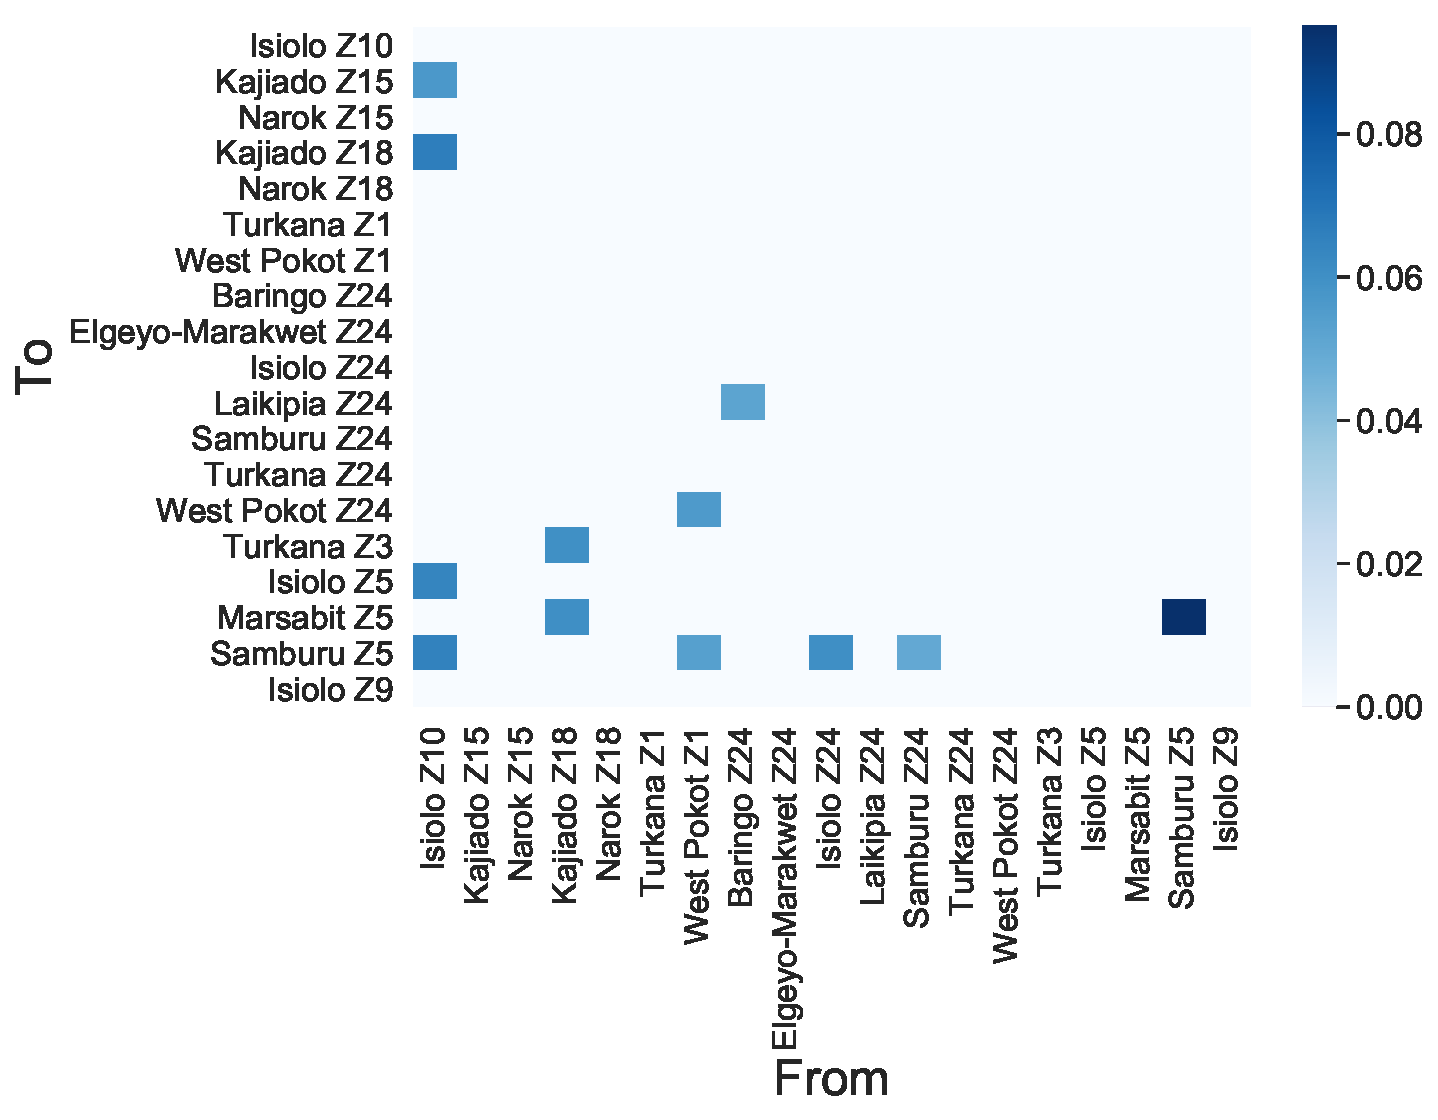
\includegraphics[trim = 20mm 0mm 0mm 0mm,width=11 cm]{figures/GCheatmap2.pdf}
	\caption{Granger causality of NDVI anomaly from each region to each other region, computed on the MODIS data, measured as improvement in $R^2$-score when observations from region `From' are added to the AR model for forecasting region `To' at a lead time of 4 weeks. Only substantial Granger causalities are shown, i.e.~those with $\Delta R^2>0.05$.} \label{fig:GCheatmap}
\end{figure}



\newpage
\section*{References}

\bibliography{mybibfile}

\end{document}








%\paragraph{Usage} Once the package is properly installed, you can use the document class \emph{elsarticle} to create a manuscript. Please make sure that your manuscript follows the guidelines in the Guide for Authors of the relevant journal. It is not necessary to typeset your manuscript in exactly the same way as an article, unless you are submitting to a camera-ready copy (CRC) journal.

%The author names and affiliations could be formatted in two ways:
%\begin{enumerate}[(1)]
%\item Group the authors per affiliation.
%\item Use footnotes to indicate the affiliations.
%\end{enumerate}


